\documentclass[11pt,a4paper]{article}
\usepackage[utf8]{inputenc}
\usepackage[T1]{fontenc}
\usepackage{lmodern}
\usepackage{textcomp}
\usepackage{amsmath,amssymb}
\usepackage{graphicx}
\usepackage{booktabs}
\usepackage{longtable}
\usepackage{array}
\usepackage{listings}
\usepackage{xcolor}
\usepackage[margin=1in]{geometry}
\usepackage{float}
\usepackage[hidelinks,breaklinks]{hyperref}
\usepackage{microtype}
\setlength{\parskip}{4pt}
\lstset{basicstyle=\ttfamily\scriptsize,breaklines=true,breakatwhitespace=false,
  postbreak=\mbox{\textcolor{gray}{$\hookrightarrow$}\space},frame=single,
  framerule=0.3pt,rulecolor=\color{gray!60},columns=fullflexible,keepspaces=true,
  showstringspaces=false,numbers=none,xleftmargin=4pt,xrightmargin=4pt,
  literate={\_}{{\_}}1}
\graphicspath{{figures/}}
\providecommand{\tightlist}{}
\title{Supplementary material: Baryonic Suppression of the Matter Power Spectrum: Literature Bracket and CRK-HACC Emulator Predictions}
\author{HEP-Genesis-Agent session record \\ \small Project: ramp-research-baryonic-pk}
\date{2026-10-23}
\begin{document}
\maketitle
\noindent\textit{\small Supplementary material, generated mechanically from the session record: it lists exactly what ran, in order, without interpretation.}
\vspace{1em}



\appendix
\section{Implementation details}
\label{app:impl}
This appendix is generated mechanically from the session record; it lists exactly what ran, in order, without interpretation.
\subsection{Session}
\begin{itemize}
  \item Source: cli client; conversation \texttt{59809a7f}
  \item Started: 2026-10-17 11:00:39; report generated: 2026-10-23 11:10:24
  \item Project: ramp-research-baryonic-pk (\texttt{/\allowbreak{}Users/\allowbreak{}nramachandra/\allowbreak{}hep-genesis-testing/\allowbreak{}projects/\allowbreak{}ramp-research-baryonic-pk})
  \item Compute execution site(s) selected in the session: local
  \item 2 user turn(s), 209 tool call(s) (0 returned errors), 15 figure(s), 31 data file(s)
\end{itemize}
\subsection{Models}
\begin{longtable}{@{}p{0.16\textwidth}p{0.34\textwidth}p{0.44\textwidth}@{}}
\toprule Stage & Model & Endpoint \\ \midrule \endhead
quick & \texttt{claude-opus-5-5} & \texttt{https:\allowbreak{}/\allowbreak{}/\allowbreak{}mag.genesis.americansciencecloud.org/\allowbreak{}v1} \\
report & \texttt{claude-opus-5-5} & \texttt{https:\allowbreak{}/\allowbreak{}/\allowbreak{}mag.genesis.americansciencecloud.org/\allowbreak{}v1} \\
coder & \texttt{claude-opus-5-5} & \texttt{https:\allowbreak{}/\allowbreak{}/\allowbreak{}mag.genesis.americansciencecloud.org/\allowbreak{}v1} \\
\bottomrule\end{longtable}
\subsection{MCP servers}
\begin{longtable}{@{}p{0.22\textwidth}p{0.12\textwidth}p{0.6\textwidth}@{}}
\toprule Server & Transport & Location \\ \midrule \endhead
hep-research-aid & stdio & \texttt{python -m hep\_\allowbreak{}genesis.domain.mcp\_\allowbreak{}server} \\
alcf-tools & stdio & \texttt{python -m hep\_\allowbreak{}genesis.iri.alcf.mcp\_\allowbreak{}server} \\
nersc-tools & stdio & \texttt{python -m hep\_\allowbreak{}genesis.iri.nersc.mcp\_\allowbreak{}server} \\
\bottomrule\end{longtable}
\subsection{Tool-call log}
Chronological; arguments and results are truncated for space (the full record is in the project's \texttt{provenance/} folder).
\begin{longtable}{@{}p{0.04\textwidth}p{0.22\textwidth}p{0.36\textwidth}p{0.32\textwidth}@{}}
\toprule \# & Tool & Arguments & Outcome \\ \midrule \endhead
1 & \texttt{hep-research-aid}\newline\texttt{list\_\allowbreak{}agent\_\allowbreak{}files} & \texttt{\{\}\allowbreak{}} & \texttt{[]\allowbreak{}} \\
2 & \texttt{hep-research-aid}\newline\texttt{list\_\allowbreak{}input\_\allowbreak{}files} & \texttt{\{\}\allowbreak{}} & \texttt{\{   ''status'':\allowbreak{} ''success'',\allowbreak{}   ''files'':\allowbreak{} []\allowbreak{},\allowbreak{}   ''usage'':\allowbreak{} ''Pass any of these filenames to load\_\allowbreak{}table\_\allowbreak{}data()\allowbreak{}.'' \}\allowbreak{}} \\
3 & \texttt{hep-research-aid}\newline\texttt{list\_\allowbreak{}datasets} & \texttt{\{\}\allowbreak{}} & \texttt{\{'count':\allowbreak{} 0,\allowbreak{} 'datasets':\allowbreak{} []\allowbreak{}\}\allowbreak{}} \\
4 & \texttt{hep-research-aid}\newline\texttt{list\_\allowbreak{}files} & \texttt{\{\}\allowbreak{}} & \texttt{Files in .:\allowbreak{}   - .git   - .gitignore   - ISSUES.md   - SCOPE.md   - docs   - downloads   - logs   - projects   - reports   - research-results   - runs   - scripts   - venvs   - workspace} \\
5 & \texttt{hep-research-aid}\newline\texttt{get\_\allowbreak{}dispatch} & \texttt{\{\}\allowbreak{}} & \texttt{Dispatch:\allowbreak{} local execution.} \\
6 & \texttt{local}\newline\texttt{search\_\allowbreak{}arxiv\_\allowbreak{}abstracts} & \texttt{\{''query'':\allowbreak{} ''baryonic suppression matter power spectrum AGN feedback hydrodynamical simulations'',\allowbreak{} ''max\_\allowbreak{}results'':\allowbreak{} 8\}\allowbreak{}} & \texttt{Search failed:\allowbreak{} Page request resulted in HTTP 429 (https:\allowbreak{}/\allowbreak{}/\allowbreak{}export.arxiv.org/\allowbreak{}api/\allowbreak{}query?search\_\allowbreak{}query=\allowbreak{}baryonic+suppression+matter+power+spectrum+AGN+feedback+hydrodynamical+simulations\&id\_\allowbreak{}list=\allowbreak{}\&sortBy=\allowbreak{}rel\ldots{}\allowbreak{}} \\
7 & \texttt{local}\newline\texttt{search\_\allowbreak{}arxiv\_\allowbreak{}abstracts} & \texttt{\{''query'':\allowbreak{} ''emulator baryonic effects matter power spectrum ratio'',\allowbreak{} ''max\_\allowbreak{}results'':\allowbreak{} 8\}\allowbreak{}} & \texttt{Search failed:\allowbreak{} Page request resulted in HTTP 429 (https:\allowbreak{}/\allowbreak{}/\allowbreak{}export.arxiv.org/\allowbreak{}api/\allowbreak{}query?search\_\allowbreak{}query=\allowbreak{}emulator+baryonic+effects+matter+power+spectrum+ratio\&id\_\allowbreak{}list=\allowbreak{}\&sortBy=\allowbreak{}relevance\&sortOrder=\allowbreak{}descending\&s\ldots{}\allowbreak{}} \\
8 & \texttt{local}\newline\texttt{search\_\allowbreak{}arxiv\_\allowbreak{}abstracts} & \texttt{\{''query'':\allowbreak{} ''weak lensing S8 baryonic feedback constraints cosmic shear'',\allowbreak{} ''max\_\allowbreak{}results'':\allowbreak{} 8\}\allowbreak{}} & \texttt{Search failed:\allowbreak{} Page request resulted in HTTP 429 (https:\allowbreak{}/\allowbreak{}/\allowbreak{}export.arxiv.org/\allowbreak{}api/\allowbreak{}query?search\_\allowbreak{}query=\allowbreak{}weak+lensing+S8+baryonic+feedback+constraints+cosmic+shear\&id\_\allowbreak{}list=\allowbreak{}\&sortBy=\allowbreak{}relevance\&sortOrder=\allowbreak{}descend\ldots{}\allowbreak{}} \\
9 & \texttt{hep-research-aid}\newline\texttt{search\_\allowbreak{}arxiv} & \texttt{\{''query'':\allowbreak{} ''baryonic suppression matter power spectrum AGN feedback'',\allowbreak{} ''max\_\allowbreak{}results'':\allowbreak{} 8\}\allowbreak{}} & \texttt{Found 8 papers matching query:\allowbreak{} 'baryonic suppression matter power spectrum AGN feedback' (source:\allowbreak{} OpenAlex)\allowbreak{}  Paper 1:\allowbreak{} arXiv ID:\allowbreak{} 1801.08559 Title:\allowbreak{} The impact of baryons on the matter power spectrum fro\ldots{}\allowbreak{}} \\
10 & \texttt{hep-research-aid}\newline\texttt{search\_\allowbreak{}arxiv} & \texttt{\{''query'':\allowbreak{} ''baryonic effects matter power spectrum emulator'',\allowbreak{} ''max\_\allowbreak{}results'':\allowbreak{} 8\}\allowbreak{}} & \texttt{Found 8 papers matching query:\allowbreak{} 'baryonic effects matter power spectrum emulator' (source:\allowbreak{} OpenAlex)\allowbreak{}  Paper 1:\allowbreak{} arXiv ID:\allowbreak{} 2108.08863 Title:\allowbreak{} Emulation of baryonic effects on the matter power spectrum and\ldots{}\allowbreak{}} \\
11 & \texttt{hep-research-aid}\newline\texttt{search\_\allowbreak{}arxiv} & \texttt{\{''query'':\allowbreak{} ''cosmic shear baryonic feedback S8 tension'',\allowbreak{} ''max\_\allowbreak{}results'':\allowbreak{} 8\}\allowbreak{}} & \texttt{Found 8 papers matching query:\allowbreak{} 'cosmic shear baryonic feedback S8 tension' (source:\allowbreak{} OpenAlex)\allowbreak{}  Paper 1:\allowbreak{} arXiv ID:\allowbreak{} 2309.07959 Title:\allowbreak{} The FLAMINGO project:\allowbreak{} revisiting the S 8 tension and the role of bar\ldots{}\allowbreak{}} \\
12 & \texttt{hep-research-aid}\newline\texttt{search\_\allowbreak{}arxiv} & \texttt{\{''max\_\allowbreak{}results'':\allowbreak{} 6,\allowbreak{} ''query'':\allowbreak{} ''kinetic Sunyaev-Zeldovich weak lensing strong baryonic feedback suppression''\}\allowbreak{}} & \texttt{Found 6 papers matching query:\allowbreak{} 'kinetic Sunyaev-Zeldovich weak lensing strong baryonic feedback suppression' (source:\allowbreak{} OpenAlex)\allowbreak{}  Paper 1:\allowbreak{} arXiv ID:\allowbreak{} 2404.06098 Title:\allowbreak{} Weak lensing combined with the kin\ldots{}\allowbreak{}} \\
13 & \texttt{hep-research-aid}\newline\texttt{search\_\allowbreak{}arxiv} & \texttt{\{''max\_\allowbreak{}results'':\allowbreak{} 6,\allowbreak{} ''query'':\allowbreak{} ''SP(k)\allowbreak{} baryon fraction halo power spectrum suppression relation''\}\allowbreak{}} & \texttt{Found 6 papers matching query:\allowbreak{} 'SP(k)\allowbreak{} baryon fraction halo power spectrum suppression relation' (source:\allowbreak{} OpenAlex)\allowbreak{}  Paper 1:\allowbreak{} arXiv ID:\allowbreak{} 1510.06034 Title:\allowbreak{} A new method to quantify the effects of baryons\ldots{}\allowbreak{}} \\
14 & \texttt{hep-research-aid}\newline\texttt{search\_\allowbreak{}arxiv} & \texttt{\{''max\_\allowbreak{}results'':\allowbreak{} 6,\allowbreak{} ''query'':\allowbreak{} ''BACCO baryonification emulator power spectrum''\}\allowbreak{}} & \texttt{Found 6 papers matching query:\allowbreak{} 'BACCO baryonification emulator power spectrum' (source:\allowbreak{} arXiv API)\allowbreak{}  Paper 1:\allowbreak{} arXiv ID:\allowbreak{} 2011.15018v1 Title:\allowbreak{} The BACCO Simulation Project:\allowbreak{} A baryonification emulator with\ldots{}\allowbreak{}} \\
15 & \texttt{hep-research-aid}\newline\texttt{search\_\allowbreak{}arxiv} & \texttt{\{''max\_\allowbreak{}results'':\allowbreak{} 5,\allowbreak{} ''query'':\allowbreak{} ''non-linear modification matter power spectrum S8 tension Amon Efstathiou''\}\allowbreak{}} & \texttt{Found 5 papers matching query:\allowbreak{} 'non-linear modification matter power spectrum S8 tension Amon Efstathiou' (source:\allowbreak{} arXiv API)\allowbreak{}  Paper 1:\allowbreak{} arXiv ID:\allowbreak{} 2305.09827v1 Title:\allowbreak{} A non-linear solution to the \$S\_\allowbreak{}8\$\ldots{}\allowbreak{}} \\
16 & \texttt{hep-research-aid}\newline\texttt{search\_\allowbreak{}arxiv} & \texttt{\{''max\_\allowbreak{}results'':\allowbreak{} 5,\allowbreak{} ''query'':\allowbreak{} ''van Daalen effects of galaxy formation on the matter power spectrum OWLS''\}\allowbreak{}} & \texttt{Found 5 papers matching query:\allowbreak{} 'van Daalen effects of galaxy formation on the matter power spectrum OWLS' (source:\allowbreak{} arXiv API)\allowbreak{}  Paper 1:\allowbreak{} arXiv ID:\allowbreak{} 1104.1174v2 Title:\allowbreak{} The effects of galaxy formation on \ldots{}\allowbreak{}} \\
17 & \texttt{hep-research-aid}\newline\texttt{list\_\allowbreak{}input\_\allowbreak{}files} & \texttt{\{\}\allowbreak{}} & \texttt{\{   ''status'':\allowbreak{} ''success'',\allowbreak{}   ''files'':\allowbreak{} []\allowbreak{},\allowbreak{}   ''usage'':\allowbreak{} ''Pass any of these filenames to load\_\allowbreak{}table\_\allowbreak{}data()\allowbreak{}.'' \}\allowbreak{}} \\
18 & \texttt{hep-research-aid}\newline\texttt{list\_\allowbreak{}agent\_\allowbreak{}files} & \texttt{\{\}\allowbreak{}} & \texttt{[]\allowbreak{}} \\
19 & \texttt{hep-research-aid}\newline\texttt{get\_\allowbreak{}dispatch} & \texttt{\{\}\allowbreak{}} & \texttt{Dispatch:\allowbreak{} local execution.} \\
20 & \texttt{hep-research-aid}\newline\texttt{run\_\allowbreak{}test\_\allowbreak{}job} & \texttt{\{''n'':\allowbreak{} 1000,\allowbreak{} ''seed'':\allowbreak{} 1\}\allowbreak{}} & \texttt{\{   ''status'':\allowbreak{} ''success'',\allowbreak{}   ''distribution'':\allowbreak{} ''normal'',\allowbreak{}   ''params'':\allowbreak{} \{     ''mu'':\allowbreak{} 0.0,\allowbreak{}     ''sigma'':\allowbreak{} 1.0   \}\allowbreak{},\allowbreak{}   ''seed'':\allowbreak{} 1,\allowbreak{}   ''summary'':\allowbreak{} \{     ''count'':\allowbreak{} 1000,\allowbreak{}     ''mean'':\allowbreak{} -0.013222050876781842,\allowbreak{}     ''stdev'':\allowbreak{} 1\ldots{}\allowbreak{}} \\
21 & \texttt{hep-research-aid}\newline\texttt{get\_\allowbreak{}paper\_\allowbreak{}figures} & \texttt{\{''paper\_\allowbreak{}id'':\allowbreak{} ''2108.08863'',\allowbreak{} ''max\_\allowbreak{}figures'':\allowbreak{} 8,\allowbreak{} ''output\_\allowbreak{}dir'':\allowbreak{} ''/\allowbreak{}Users/\allowbreak{}nramachandra/\allowbreak{}hep-genesis-testing/\allowbreak{}projects/\allowbreak{}ramp-research-baryonic-pk/\allowbreak{}runs/\allowbreak{}261017\_\allowbreak{}110039''\}\allowbreak{}} & \texttt{\{''status'':\allowbreak{} ''success'',\allowbreak{} ''files'':\allowbreak{} [''/\allowbreak{}Users/\allowbreak{}nramachandra/\allowbreak{}hep-genesis-testing/\allowbreak{}projects/\allowbreak{}ramp-research-baryonic-pk/\allowbreak{}runs/\allowbreak{}261017\_\allowbreak{}110039/\allowbreak{}figures\_\allowbreak{}2108.08863/\allowbreak{}fig01.png'',\allowbreak{} ''/\allowbreak{}Users/\allowbreak{}nramachandra/\allowbreak{}hep-genesis-testing/\allowbreak{}p\ldots{}\allowbreak{}} [Fig. 1, 2, 3, 4, 5, 6, 7, 8] \\
22 & \texttt{local}\newline\texttt{download\_\allowbreak{}arxiv\_\allowbreak{}full\_\allowbreak{}text} & \texttt{\{''arxiv\_\allowbreak{}id'':\allowbreak{} ''2206.11794'',\allowbreak{} ''output\_\allowbreak{}dir'':\allowbreak{} ''/\allowbreak{}Users/\allowbreak{}nramachandra/\allowbreak{}hep-genesis-testing/\allowbreak{}projects/\allowbreak{}ramp-research-baryonic-pk/\allowbreak{}runs/\allowbreak{}261017\_\allowbreak{}110039''\}\allowbreak{}} & \texttt{Downloaded:\allowbreak{} /\allowbreak{}Users/\allowbreak{}nramachandra/\allowbreak{}hep-genesis-testing/\allowbreak{}projects/\allowbreak{}ramp-research-baryonic-pk/\allowbreak{}runs/\allowbreak{}261017\_\allowbreak{}110039/\allowbreak{}2206.11794.txt} \\
23 & \texttt{local}\newline\texttt{download\_\allowbreak{}arxiv\_\allowbreak{}full\_\allowbreak{}text} & \texttt{\{''arxiv\_\allowbreak{}id'':\allowbreak{} ''1104.1174'',\allowbreak{} ''output\_\allowbreak{}dir'':\allowbreak{} ''/\allowbreak{}Users/\allowbreak{}nramachandra/\allowbreak{}hep-genesis-testing/\allowbreak{}projects/\allowbreak{}ramp-research-baryonic-pk/\allowbreak{}runs/\allowbreak{}261017\_\allowbreak{}110039''\}\allowbreak{}} & \texttt{Downloaded:\allowbreak{} /\allowbreak{}Users/\allowbreak{}nramachandra/\allowbreak{}hep-genesis-testing/\allowbreak{}projects/\allowbreak{}ramp-research-baryonic-pk/\allowbreak{}runs/\allowbreak{}261017\_\allowbreak{}110039/\allowbreak{}1104.1174.txt} \\
24 & \texttt{local}\newline\texttt{download\_\allowbreak{}arxiv\_\allowbreak{}full\_\allowbreak{}text} & \texttt{\{''arxiv\_\allowbreak{}id'':\allowbreak{} ''2305.09827'',\allowbreak{} ''output\_\allowbreak{}dir'':\allowbreak{} ''/\allowbreak{}Users/\allowbreak{}nramachandra/\allowbreak{}hep-genesis-testing/\allowbreak{}projects/\allowbreak{}ramp-research-baryonic-pk/\allowbreak{}runs/\allowbreak{}261017\_\allowbreak{}110039''\}\allowbreak{}} & \texttt{Downloaded:\allowbreak{} /\allowbreak{}Users/\allowbreak{}nramachandra/\allowbreak{}hep-genesis-testing/\allowbreak{}projects/\allowbreak{}ramp-research-baryonic-pk/\allowbreak{}runs/\allowbreak{}261017\_\allowbreak{}110039/\allowbreak{}2305.09827.txt} \\
25 & \texttt{local}\newline\texttt{download\_\allowbreak{}arxiv\_\allowbreak{}full\_\allowbreak{}text} & \texttt{\{''arxiv\_\allowbreak{}id'':\allowbreak{} ''2108.08863'',\allowbreak{} ''output\_\allowbreak{}dir'':\allowbreak{} ''/\allowbreak{}Users/\allowbreak{}nramachandra/\allowbreak{}hep-genesis-testing/\allowbreak{}projects/\allowbreak{}ramp-research-baryonic-pk/\allowbreak{}runs/\allowbreak{}261017\_\allowbreak{}110039''\}\allowbreak{}} & \texttt{Downloaded:\allowbreak{} /\allowbreak{}Users/\allowbreak{}nramachandra/\allowbreak{}hep-genesis-testing/\allowbreak{}projects/\allowbreak{}ramp-research-baryonic-pk/\allowbreak{}runs/\allowbreak{}261017\_\allowbreak{}110039/\allowbreak{}2108.08863.txt} \\
26 & \texttt{local}\newline\texttt{download\_\allowbreak{}arxiv\_\allowbreak{}full\_\allowbreak{}text} & \texttt{\{''arxiv\_\allowbreak{}id'':\allowbreak{} ''1906.00968'',\allowbreak{} ''output\_\allowbreak{}dir'':\allowbreak{} ''/\allowbreak{}Users/\allowbreak{}nramachandra/\allowbreak{}hep-genesis-testing/\allowbreak{}projects/\allowbreak{}ramp-research-baryonic-pk/\allowbreak{}runs/\allowbreak{}261017\_\allowbreak{}110039''\}\allowbreak{}} & \texttt{Downloaded:\allowbreak{} /\allowbreak{}Users/\allowbreak{}nramachandra/\allowbreak{}hep-genesis-testing/\allowbreak{}projects/\allowbreak{}ramp-research-baryonic-pk/\allowbreak{}runs/\allowbreak{}261017\_\allowbreak{}110039/\allowbreak{}1906.00968.txt} \\
27 & \texttt{local}\newline\texttt{download\_\allowbreak{}arxiv\_\allowbreak{}full\_\allowbreak{}text} & \texttt{\{''arxiv\_\allowbreak{}id'':\allowbreak{} ''2309.07959'',\allowbreak{} ''output\_\allowbreak{}dir'':\allowbreak{} ''/\allowbreak{}Users/\allowbreak{}nramachandra/\allowbreak{}hep-genesis-testing/\allowbreak{}projects/\allowbreak{}ramp-research-baryonic-pk/\allowbreak{}runs/\allowbreak{}261017\_\allowbreak{}110039''\}\allowbreak{}} & \texttt{Downloaded:\allowbreak{} /\allowbreak{}Users/\allowbreak{}nramachandra/\allowbreak{}hep-genesis-testing/\allowbreak{}projects/\allowbreak{}ramp-research-baryonic-pk/\allowbreak{}runs/\allowbreak{}261017\_\allowbreak{}110039/\allowbreak{}2309.07959.txt} \\
28 & \texttt{local}\newline\texttt{download\_\allowbreak{}arxiv\_\allowbreak{}full\_\allowbreak{}text} & \texttt{\{''arxiv\_\allowbreak{}id'':\allowbreak{} ''2410.17109'',\allowbreak{} ''output\_\allowbreak{}dir'':\allowbreak{} ''/\allowbreak{}Users/\allowbreak{}nramachandra/\allowbreak{}hep-genesis-testing/\allowbreak{}projects/\allowbreak{}ramp-research-baryonic-pk/\allowbreak{}runs/\allowbreak{}261017\_\allowbreak{}110039''\}\allowbreak{}} & \texttt{Downloaded:\allowbreak{} /\allowbreak{}Users/\allowbreak{}nramachandra/\allowbreak{}hep-genesis-testing/\allowbreak{}projects/\allowbreak{}ramp-research-baryonic-pk/\allowbreak{}runs/\allowbreak{}261017\_\allowbreak{}110039/\allowbreak{}2410.17109.txt} \\
29 & \texttt{local}\newline\texttt{download\_\allowbreak{}arxiv\_\allowbreak{}full\_\allowbreak{}text} & \texttt{\{''arxiv\_\allowbreak{}id'':\allowbreak{} ''2309.06479'',\allowbreak{} ''output\_\allowbreak{}dir'':\allowbreak{} ''/\allowbreak{}Users/\allowbreak{}nramachandra/\allowbreak{}hep-genesis-testing/\allowbreak{}projects/\allowbreak{}ramp-research-baryonic-pk/\allowbreak{}runs/\allowbreak{}261017\_\allowbreak{}110039''\}\allowbreak{}} & \texttt{Downloaded:\allowbreak{} /\allowbreak{}Users/\allowbreak{}nramachandra/\allowbreak{}hep-genesis-testing/\allowbreak{}projects/\allowbreak{}ramp-research-baryonic-pk/\allowbreak{}runs/\allowbreak{}261017\_\allowbreak{}110039/\allowbreak{}2309.06479.txt} \\
30 & \texttt{local}\newline\texttt{download\_\allowbreak{}arxiv\_\allowbreak{}full\_\allowbreak{}text} & \texttt{\{''arxiv\_\allowbreak{}id'':\allowbreak{} ''2404.06098'',\allowbreak{} ''output\_\allowbreak{}dir'':\allowbreak{} ''/\allowbreak{}Users/\allowbreak{}nramachandra/\allowbreak{}hep-genesis-testing/\allowbreak{}projects/\allowbreak{}ramp-research-baryonic-pk/\allowbreak{}runs/\allowbreak{}261017\_\allowbreak{}110039''\}\allowbreak{}} & \texttt{Downloaded:\allowbreak{} /\allowbreak{}Users/\allowbreak{}nramachandra/\allowbreak{}hep-genesis-testing/\allowbreak{}projects/\allowbreak{}ramp-research-baryonic-pk/\allowbreak{}runs/\allowbreak{}261017\_\allowbreak{}110039/\allowbreak{}2404.06098.txt} \\
31 & \texttt{local}\newline\texttt{download\_\allowbreak{}arxiv\_\allowbreak{}full\_\allowbreak{}text} & \texttt{\{''arxiv\_\allowbreak{}id'':\allowbreak{} ''1104.1174'',\allowbreak{} ''output\_\allowbreak{}dir'':\allowbreak{} ''/\allowbreak{}Users/\allowbreak{}nramachandra/\allowbreak{}hep-genesis-testing/\allowbreak{}projects/\allowbreak{}ramp-research-baryonic-pk/\allowbreak{}runs/\allowbreak{}261017\_\allowbreak{}110039''\}\allowbreak{}} & \texttt{Downloaded:\allowbreak{} /\allowbreak{}Users/\allowbreak{}nramachandra/\allowbreak{}hep-genesis-testing/\allowbreak{}projects/\allowbreak{}ramp-research-baryonic-pk/\allowbreak{}runs/\allowbreak{}261017\_\allowbreak{}110039/\allowbreak{}1104.1174.txt} \\
32 & \texttt{local}\newline\texttt{download\_\allowbreak{}arxiv\_\allowbreak{}full\_\allowbreak{}text} & \texttt{\{''arxiv\_\allowbreak{}id'':\allowbreak{} ''1801.08559'',\allowbreak{} ''output\_\allowbreak{}dir'':\allowbreak{} ''/\allowbreak{}Users/\allowbreak{}nramachandra/\allowbreak{}hep-genesis-testing/\allowbreak{}projects/\allowbreak{}ramp-research-baryonic-pk/\allowbreak{}runs/\allowbreak{}261017\_\allowbreak{}110039''\}\allowbreak{}} & \texttt{Downloaded:\allowbreak{} /\allowbreak{}Users/\allowbreak{}nramachandra/\allowbreak{}hep-genesis-testing/\allowbreak{}projects/\allowbreak{}ramp-research-baryonic-pk/\allowbreak{}runs/\allowbreak{}261017\_\allowbreak{}110039/\allowbreak{}1801.08559.txt} \\
33 & \texttt{local}\newline\texttt{read\_\allowbreak{}arxiv\_\allowbreak{}chunk} & \texttt{\{''filepath'':\allowbreak{} ''/\allowbreak{}Users/\allowbreak{}nramachandra/\allowbreak{}hep-genesis-testing/\allowbreak{}projects/\allowbreak{}ramp-research-baryonic-pk/\allowbreak{}runs/\allowbreak{}261017\_\allowbreak{}110039/\allowbreak{}2206.11794.txt'',\allowbreak{} ''length'':\allowbreak{} 9000\}\allowbreak{}} & \texttt{[chars 0-9000 of 65221]\allowbreak{} (more available,\allowbreak{} next start=\allowbreak{}9000)\allowbreak{}  Title:\allowbreak{} A non-linear solution to the \$S\_\allowbreak{}8\$ tension? Authors:\allowbreak{} Alexandra Amon,\allowbreak{} George Efstathiou Year:\allowbreak{} 2022 arXiv ID:\allowbreak{} 2206.11794  =\allowbreak{}=\allowbreak{}=\allowbreak{}=\allowbreak{}=\allowbreak{}=\allowbreak{}=\allowbreak{}=\allowbreak{}=\allowbreak{}=\allowbreak{}=\allowbreak{}=\allowbreak{}=\allowbreak{}=\allowbreak{}\ldots{}\allowbreak{}} \\
34 & \texttt{local}\newline\texttt{download\_\allowbreak{}arxiv\_\allowbreak{}full\_\allowbreak{}text} & \texttt{\{''arxiv\_\allowbreak{}id'':\allowbreak{} ''2403.12967'',\allowbreak{} ''output\_\allowbreak{}dir'':\allowbreak{} ''/\allowbreak{}Users/\allowbreak{}nramachandra/\allowbreak{}hep-genesis-testing/\allowbreak{}projects/\allowbreak{}ramp-research-baryonic-pk/\allowbreak{}runs/\allowbreak{}261017\_\allowbreak{}110039''\}\allowbreak{}} & \texttt{Downloaded:\allowbreak{} /\allowbreak{}Users/\allowbreak{}nramachandra/\allowbreak{}hep-genesis-testing/\allowbreak{}projects/\allowbreak{}ramp-research-baryonic-pk/\allowbreak{}runs/\allowbreak{}261017\_\allowbreak{}110039/\allowbreak{}2403.12967.txt} \\
35 & \texttt{local}\newline\texttt{read\_\allowbreak{}arxiv\_\allowbreak{}chunk} & \texttt{\{''filepath'':\allowbreak{} ''/\allowbreak{}Users/\allowbreak{}nramachandra/\allowbreak{}hep-genesis-testing/\allowbreak{}projects/\allowbreak{}ramp-research-baryonic-pk/\allowbreak{}runs/\allowbreak{}261017\_\allowbreak{}110039/\allowbreak{}2305.09827.txt'',\allowbreak{} ''length'':\allowbreak{} 9000\}\allowbreak{}} & \texttt{[chars 0-9000 of 60884]\allowbreak{} (more available,\allowbreak{} next start=\allowbreak{}9000)\allowbreak{}  Title:\allowbreak{} A non-linear solution to the \$S\_\allowbreak{}8\$ tension II:\allowbreak{} Analysis of DES Year 3 cosmic shear Authors:\allowbreak{} Calvin Preston,\allowbreak{} Alexandra Amon,\allowbreak{} George Efs\ldots{}\allowbreak{}} \\
36 & \texttt{local}\newline\texttt{read\_\allowbreak{}arxiv\_\allowbreak{}chunk} & \texttt{\{''filepath'':\allowbreak{} ''/\allowbreak{}Users/\allowbreak{}nramachandra/\allowbreak{}hep-genesis-testing/\allowbreak{}projects/\allowbreak{}ramp-research-baryonic-pk/\allowbreak{}runs/\allowbreak{}261017\_\allowbreak{}110039/\allowbreak{}2410.17109.txt'',\allowbreak{} ''start'':\allowbreak{} 0,\allowbreak{} ''length'':\allowbreak{} 4000\}\allowbreak{}} & \texttt{[chars 0-4000 of 85813]\allowbreak{} (more available,\allowbreak{} next start=\allowbreak{}4000)\allowbreak{}  Title:\allowbreak{} The FLAMINGO project:\allowbreak{} Baryon effects on the matter power spectrum Authors:\allowbreak{} Matthieu Schaller,\allowbreak{} Joop Schaye,\allowbreak{} Roi Kugel,\allowbreak{} Jeger C. Broxter\ldots{}\allowbreak{}} \\
37 & \texttt{local}\newline\texttt{read\_\allowbreak{}arxiv\_\allowbreak{}chunk} & \texttt{\{''filepath'':\allowbreak{} ''/\allowbreak{}Users/\allowbreak{}nramachandra/\allowbreak{}hep-genesis-testing/\allowbreak{}projects/\allowbreak{}ramp-research-baryonic-pk/\allowbreak{}runs/\allowbreak{}261017\_\allowbreak{}110039/\allowbreak{}2309.07959.txt'',\allowbreak{} ''length'':\allowbreak{} 7000\}\allowbreak{}} & \texttt{[chars 0-7000 of 141592]\allowbreak{} (more available,\allowbreak{} next start=\allowbreak{}7000)\allowbreak{}  Title:\allowbreak{} The FLAMINGO project:\allowbreak{} revisiting the \$S\_\allowbreak{}8\$ tension and the role of baryonic physics Authors:\allowbreak{} Ian G. McCarthy,\allowbreak{} Jaime Salcido,\allowbreak{} Joop Sch\ldots{}\allowbreak{}} \\
38 & \texttt{local}\newline\texttt{read\_\allowbreak{}arxiv\_\allowbreak{}chunk} & \texttt{\{''filepath'':\allowbreak{} ''/\allowbreak{}Users/\allowbreak{}nramachandra/\allowbreak{}hep-genesis-testing/\allowbreak{}projects/\allowbreak{}ramp-research-baryonic-pk/\allowbreak{}runs/\allowbreak{}261017\_\allowbreak{}110039/\allowbreak{}1104.1174.txt'',\allowbreak{} ''start'':\allowbreak{} 0,\allowbreak{} ''length'':\allowbreak{} 3000\}\allowbreak{}} & \texttt{[chars 0-3000 of 99825]\allowbreak{} (more available,\allowbreak{} next start=\allowbreak{}3000)\allowbreak{}  Title:\allowbreak{} The effects of galaxy formation on the matter power spectrum:\allowbreak{} A challenge for precision cosmology Authors:\allowbreak{} Marcel P. van Daalen,\allowbreak{} Joop \ldots{}\allowbreak{}} \\
39 & \texttt{local}\newline\texttt{read\_\allowbreak{}arxiv\_\allowbreak{}chunk} & \texttt{\{''filepath'':\allowbreak{} ''/\allowbreak{}Users/\allowbreak{}nramachandra/\allowbreak{}hep-genesis-testing/\allowbreak{}projects/\allowbreak{}ramp-research-baryonic-pk/\allowbreak{}runs/\allowbreak{}261017\_\allowbreak{}110039/\allowbreak{}2404.06098.txt'',\allowbreak{} ''length'':\allowbreak{} 7000\}\allowbreak{}} & \texttt{[chars 0-7000 of 156592]\allowbreak{} (more available,\allowbreak{} next start=\allowbreak{}7000)\allowbreak{}  Title:\allowbreak{} Weak lensing combined with the kinetic Sunyaev Zel'dovich effect:\allowbreak{} A study of baryonic feedback Authors:\allowbreak{} L. Bigwood,\allowbreak{} A. Amon,\allowbreak{} A. Schne\ldots{}\allowbreak{}} \\
40 & \texttt{local}\newline\texttt{read\_\allowbreak{}arxiv\_\allowbreak{}chunk} & \texttt{\{''filepath'':\allowbreak{} ''/\allowbreak{}Users/\allowbreak{}nramachandra/\allowbreak{}hep-genesis-testing/\allowbreak{}projects/\allowbreak{}ramp-research-baryonic-pk/\allowbreak{}runs/\allowbreak{}261017\_\allowbreak{}110039/\allowbreak{}1104.1174.txt'',\allowbreak{} ''length'':\allowbreak{} 4000\}\allowbreak{}} & \texttt{[chars 0-4000 of 99825]\allowbreak{} (more available,\allowbreak{} next start=\allowbreak{}4000)\allowbreak{}  Title:\allowbreak{} The effects of galaxy formation on the matter power spectrum:\allowbreak{} A challenge for precision cosmology Authors:\allowbreak{} Marcel P. van Daalen,\allowbreak{} Joop \ldots{}\allowbreak{}} \\
41 & \texttt{local}\newline\texttt{read\_\allowbreak{}arxiv\_\allowbreak{}chunk} & \texttt{\{''filepath'':\allowbreak{} ''/\allowbreak{}Users/\allowbreak{}nramachandra/\allowbreak{}hep-genesis-testing/\allowbreak{}projects/\allowbreak{}ramp-research-baryonic-pk/\allowbreak{}runs/\allowbreak{}261017\_\allowbreak{}110039/\allowbreak{}1906.00968.txt'',\allowbreak{} ''length'':\allowbreak{} 4000\}\allowbreak{}} & \texttt{[chars 0-4000 of 135316]\allowbreak{} (more available,\allowbreak{} next start=\allowbreak{}4000)\allowbreak{}  Title:\allowbreak{} Exploring the effects of galaxy formation on matter clustering through a library of simulation power spectra Authors:\allowbreak{} Marcel P. van D\ldots{}\allowbreak{}} \\
42 & \texttt{local}\newline\texttt{read\_\allowbreak{}arxiv\_\allowbreak{}chunk} & \texttt{\{''filepath'':\allowbreak{} ''/\allowbreak{}Users/\allowbreak{}nramachandra/\allowbreak{}hep-genesis-testing/\allowbreak{}projects/\allowbreak{}ramp-research-baryonic-pk/\allowbreak{}runs/\allowbreak{}261017\_\allowbreak{}110039/\allowbreak{}2309.06479.txt'',\allowbreak{} ''length'':\allowbreak{} 4000\}\allowbreak{}} & \texttt{[chars 0-4000 of 110400]\allowbreak{} (more available,\allowbreak{} next start=\allowbreak{}4000)\allowbreak{}  Title:\allowbreak{} The contribution of massive haloes to the matter power spectrum in the presence of AGN feedback Authors:\allowbreak{} M. L. van Loon,\allowbreak{} Marcel P. va\ldots{}\allowbreak{}} \\
43 & \texttt{local}\newline\texttt{read\_\allowbreak{}arxiv\_\allowbreak{}chunk} & \texttt{\{''filepath'':\allowbreak{} ''/\allowbreak{}Users/\allowbreak{}nramachandra/\allowbreak{}hep-genesis-testing/\allowbreak{}projects/\allowbreak{}ramp-research-baryonic-pk/\allowbreak{}runs/\allowbreak{}261017\_\allowbreak{}110039/\allowbreak{}1801.08559.txt'',\allowbreak{} ''length'':\allowbreak{} 4000\}\allowbreak{}} & \texttt{[chars 0-4000 of 89998]\allowbreak{} (more available,\allowbreak{} next start=\allowbreak{}4000)\allowbreak{}  Title:\allowbreak{} The impact of baryons on the matter power spectrum from the Horizon-AGN cosmological hydrodynamical simulation Authors:\allowbreak{} Nora Elisa Chi\ldots{}\allowbreak{}} \\
44 & \texttt{local}\newline\texttt{read\_\allowbreak{}arxiv\_\allowbreak{}chunk} & \texttt{\{''filepath'':\allowbreak{} ''/\allowbreak{}Users/\allowbreak{}nramachandra/\allowbreak{}hep-genesis-testing/\allowbreak{}projects/\allowbreak{}ramp-research-baryonic-pk/\allowbreak{}runs/\allowbreak{}261017\_\allowbreak{}110039/\allowbreak{}2403.12967.txt'',\allowbreak{} ''length'':\allowbreak{} 4000\}\allowbreak{}} & \texttt{[chars 0-4000 of 110619]\allowbreak{} (more available,\allowbreak{} next start=\allowbreak{}4000)\allowbreak{}  Title:\allowbreak{} The FLAMINGO project:\allowbreak{} the coupling between baryonic feedback and cosmology in light of the \$S\_\allowbreak{}8\$ tension Authors:\allowbreak{} Willem Elbers,\allowbreak{} Carl\ldots{}\allowbreak{}} \\
45 & \texttt{local}\newline\texttt{read\_\allowbreak{}arxiv\_\allowbreak{}chunk} & \texttt{\{''filepath'':\allowbreak{} ''/\allowbreak{}Users/\allowbreak{}nramachandra/\allowbreak{}hep-genesis-testing/\allowbreak{}projects/\allowbreak{}ramp-research-baryonic-pk/\allowbreak{}runs/\allowbreak{}261017\_\allowbreak{}110039/\allowbreak{}2305.09827.txt'',\allowbreak{} ''start'':\allowbreak{} 50000,\allowbreak{} ''length'':\allowbreak{} 7000\}\allowbreak{}} & \texttt{[chars 50000-57000 of 60884]\allowbreak{} (more available,\allowbreak{} next start=\allowbreak{}57000)\allowbreak{}  s to high k and z \textgreater{}\allowbreak{} $\sim$ 1 and o?er an opportunity to potentially break the degeneracy between baryonic feedback and non- standard dark ma\ldots{}\allowbreak{}} \\
46 & \texttt{local}\newline\texttt{read\_\allowbreak{}arxiv\_\allowbreak{}chunk} & \texttt{\{''filepath'':\allowbreak{} ''/\allowbreak{}Users/\allowbreak{}nramachandra/\allowbreak{}hep-genesis-testing/\allowbreak{}projects/\allowbreak{}ramp-research-baryonic-pk/\allowbreak{}runs/\allowbreak{}261017\_\allowbreak{}110039/\allowbreak{}2404.06098.txt'',\allowbreak{} ''start'':\allowbreak{} 95000,\allowbreak{} ''length'':\allowbreak{} 8000\}\allowbreak{}} & \texttt{[chars 95000-103000 of 156592]\allowbreak{} (more available,\allowbreak{} next start=\allowbreak{}103000)\allowbreak{}  $\delta$$\xi$+/\allowbreak{}$\xi$+ 101 102 1 3 1,\allowbreak{}1 101 102 1 3  1,\allowbreak{}2 ?0.5 0.0 0.5 101 102 1 3 1,\allowbreak{}2 101 102 1 3  1,\allowbreak{}3 ?0.5 0.0 0.5 101 102 1 3 1,\allowbreak{}3 10 100 101 102 1 \ldots{}\allowbreak{}} \\
47 & \texttt{local}\newline\texttt{read\_\allowbreak{}arxiv\_\allowbreak{}chunk} & \texttt{\{''filepath'':\allowbreak{} ''/\allowbreak{}Users/\allowbreak{}nramachandra/\allowbreak{}hep-genesis-testing/\allowbreak{}projects/\allowbreak{}ramp-research-baryonic-pk/\allowbreak{}runs/\allowbreak{}261017\_\allowbreak{}110039/\allowbreak{}2309.07959.txt'',\allowbreak{} ''start'':\allowbreak{} 105000,\allowbreak{} ''length'':\allowbreak{} 8000\}\allowbreak{}} & \texttt{[chars 105000-113000 of 141592]\allowbreak{} (more available,\allowbreak{} next start=\allowbreak{}113000)\allowbreak{}  7 1.9 8.8 0.4 63.2 6.2 93.4 5.8 39.2 0.1 4.0 0.2 2.4 0.0 present and the Planck and D3A cosmologies are only in mild ten- sion with\ldots{}\allowbreak{}} \\
48 & \texttt{board}\newline\texttt{post\_\allowbreak{}dead\_\allowbreak{}end} & \texttt{\{''what'':\allowbreak{} ''Compute P\_\allowbreak{}hydro/\allowbreak{}P\_\allowbreak{}DMO at z=\allowbreak{}0 with an emulator tool'',\allowbreak{} ''why'':\allowbreak{} ''No hydro emulator exists in the catalog. The input and output file lists are empty,\allowbreak{} dispatch is local,\allowbreak{} and run\_\allowbreak{}test\_\allowbreak{}job only draws random samples (no\ldots{}\allowbreak{}} & \texttt{Recorded dead end x-01.} \\
49 & \texttt{board}\newline\texttt{post\_\allowbreak{}finding} & \texttt{\{''claim'':\allowbreak{} ''Literature value (not computed)\allowbreak{}:\allowbreak{} at z=\allowbreak{}0 the OWLS AGN model (van Daalen et al. 2011,\allowbreak{} arXiv:\allowbreak{}1104.1174)\allowbreak{} suppresses power relative to DMO by 1\% at k\textasciitilde{}\allowbreak{}0.3 h/\allowbreak{}Mpc,\allowbreak{} 10\% at k\textasciitilde{}\allowbreak{}1 h/\allowbreak{}Mpc and 30\% at k\textasciitilde{}\allowbreak{}10 h/\allowbreak{}Mpc. That gives k(\ldots{}\allowbreak{}} & \texttt{Recorded finding f-001.} \\
50 & \texttt{board}\newline\texttt{post\_\allowbreak{}finding} & \texttt{\{''claim'':\allowbreak{} ''Literature (FLAMINGO,\allowbreak{} arXiv:\allowbreak{}2410.17109,\allowbreak{} not computed)\allowbreak{}:\allowbreak{} the response gets stronger and its minimum moves to smaller scales as z falls. Lower cluster gas fractions and collimated jets (instead of thermal winds)\allowbreak{} \ldots{}\allowbreak{}} & \texttt{Recorded finding f-002.} \\
51 & \texttt{local}\newline\texttt{read\_\allowbreak{}arxiv\_\allowbreak{}chunk} & \texttt{\{''filepath'':\allowbreak{} ''/\allowbreak{}Users/\allowbreak{}nramachandra/\allowbreak{}hep-genesis-testing/\allowbreak{}projects/\allowbreak{}ramp-research-baryonic-pk/\allowbreak{}runs/\allowbreak{}261017\_\allowbreak{}110039/\allowbreak{}2108.08863.txt'',\allowbreak{} ''length'':\allowbreak{} 3500,\allowbreak{} ''start'':\allowbreak{} 0\}\allowbreak{}} & \texttt{[chars 0-3500 of 87781]\allowbreak{} (more available,\allowbreak{} next start=\allowbreak{}3500)\allowbreak{}  Title:\allowbreak{} Emulation of baryonic effects on the matter power spectrum and constraints from galaxy cluster data Authors:\allowbreak{} Sambit K. Giri,\allowbreak{} Aurel Sch\ldots{}\allowbreak{}} \\
52 & \texttt{board}\newline\texttt{post\_\allowbreak{}finding} & \texttt{\{''claim'':\allowbreak{} ''Amon \& Efstathiou (arXiv:\allowbreak{}2206.11794)\allowbreak{} model the non-linear power as P =\allowbreak{} P\_\allowbreak{}L + A\_\allowbreak{}mod(P\_\allowbreak{}NL - P\_\allowbreak{}L)\allowbreak{}. With Planck LCDM fixed,\allowbreak{} a fit to KiDS-1000 cosmic shear needs A\_\allowbreak{}mod \textasciitilde{}\allowbreak{} 0.69,\allowbreak{} which is a suppression stronger than \ldots{}\allowbreak{}} & \texttt{Recorded finding f-003.} \\
53 & \texttt{board}\newline\texttt{post\_\allowbreak{}finding} & \texttt{\{''claim'':\allowbreak{} ''Preston,\allowbreak{} Amon \& Efstathiou (arXiv:\allowbreak{}2305.09827)\allowbreak{} find that DES Y3 cosmic shear needs a milder non-linear suppression than KiDS-1000 to agree with Planck LCDM. It is still more extreme than recent simulations,\allowbreak{} and\ldots{}\allowbreak{}} & \texttt{Recorded finding f-004.} \\
54 & \texttt{board}\newline\texttt{post\_\allowbreak{}finding} & \texttt{\{''claim'':\allowbreak{} ''FLAMINGO (McCarthy et al.,\allowbreak{} arXiv:\allowbreak{}2309.07959)\allowbreak{} compares its full suite,\allowbreak{} including extreme feedback variants,\allowbreak{} with cosmic shear,\allowbreak{} CMB lensing,\allowbreak{} tSZ and their cross-spectra. It concludes that baryonic effects are no\ldots{}\allowbreak{}} & \texttt{Recorded finding f-005.} \\
55 & \texttt{board}\newline\texttt{post\_\allowbreak{}finding} & \texttt{\{''claim'':\allowbreak{} ''Bigwood et al. (arXiv:\allowbreak{}2404.06098)\allowbreak{} fit DES Y3 WL + ACT DR5 kSZ with BCEmu baryonification. They get S8 =\allowbreak{} 0.823+0.019-0.020,\allowbreak{} higher than WL alone. The fit prefers a mean feedback scenario more extreme than most \ldots{}\allowbreak{}} & \texttt{Recorded finding f-006.} \\
56 & \texttt{local}\newline\texttt{cite} & \texttt{\{''arxiv\_\allowbreak{}id'':\allowbreak{} ''1104.1174'',\allowbreak{} ''note'':\allowbreak{} ''[\textbackslash{}\allowbreak{}''from 1\% at k $\approx$ 0.3 h Mpc- 1\textbackslash{}\allowbreak{}'',\allowbreak{} \textbackslash{}\allowbreak{}''Therefore,\allowbreak{} baryons,\allowbreak{} and particularly AGN feedback,\allowbreak{} cannot be\textbackslash{}\allowbreak{}'',\allowbreak{} \textbackslash{}\allowbreak{}''ignored in theoretical power spectra for k\textbackslash{}\allowbreak{}'']\allowbreak{}'',\allowbreak{} ''bib\_\allowbreak{}path'':\allowbreak{} ''/\allowbreak{}Users/\allowbreak{}nramachandra/\allowbreak{}he\ldots{}\allowbreak{}} & \texttt{Cited:\allowbreak{} The effects of galaxy formation on the matter power spectrum:\allowbreak{} A challenge for precision cosmology (\textbackslash{}\allowbreak{}cite\{arxiv11041174\}\allowbreak{})\allowbreak{}} \\
57 & \texttt{local}\newline\texttt{cite} & \texttt{\{''arxiv\_\allowbreak{}id'':\allowbreak{} ''1906.00968'',\allowbreak{} ''note'':\allowbreak{} ''[\textbackslash{}\allowbreak{}''given only the mean baryon fraction in galaxy groups.\textbackslash{}\allowbreak{}'',\allowbreak{} \textbackslash{}\allowbreak{}''reducing the power by 1\% at a Fourier scale of k =\allowbreak{} 0 . 3 h Mpc- 1 to\textbackslash{}\allowbreak{}'']\allowbreak{}'',\allowbreak{} ''bib\_\allowbreak{}path'':\allowbreak{} ''/\allowbreak{}Users/\allowbreak{}nramachandra/\allowbreak{}hep-genesis-tes\ldots{}\allowbreak{}} & \texttt{Cited:\allowbreak{} Exploring the effects of galaxy formation on matter clustering through a library of simulation power spectra (\textbackslash{}\allowbreak{}cite\{arxiv190600968\}\allowbreak{})\allowbreak{}} \\
58 & \texttt{local}\newline\texttt{cite} & \texttt{\{''arxiv\_\allowbreak{}id'':\allowbreak{} ''2309.06479'',\allowbreak{} ''note'':\allowbreak{} ''[\textbackslash{}\allowbreak{}''by ejecting matter from within r500,\allowbreak{}c to r200,\allowbreak{}m and\textbackslash{}\allowbreak{}'',\allowbreak{} \textbackslash{}\allowbreak{}''dominate the power spectrum,\allowbreak{} while on smaller scales the combined\textbackslash{}\allowbreak{}'']\allowbreak{}'',\allowbreak{} ''bib\_\allowbreak{}path'':\allowbreak{} ''/\allowbreak{}Users/\allowbreak{}nramachandra/\allowbreak{}hep-genesis-testing/\allowbreak{}\ldots{}\allowbreak{}} & \texttt{Cited:\allowbreak{} The contribution of massive haloes to the matter power spectrum in the presence of AGN feedback (\textbackslash{}\allowbreak{}cite\{arxiv230906479\}\allowbreak{})\allowbreak{}} \\
59 & \texttt{local}\newline\texttt{cite} & \texttt{\{''arxiv\_\allowbreak{}id'':\allowbreak{} ''1801.08559'',\allowbreak{} ''note'':\allowbreak{} ''[\textbackslash{}\allowbreak{}''due to an interplay between AGN feedback\textbackslash{}\allowbreak{}'',\allowbreak{} \textbackslash{}\allowbreak{}''of \textless{}\allowbreak{} 15\% at z =\allowbreak{} 0\textbackslash{}\allowbreak{}'']\allowbreak{}'',\allowbreak{} ''bib\_\allowbreak{}path'':\allowbreak{} ''/\allowbreak{}Users/\allowbreak{}nramachandra/\allowbreak{}hep-genesis-testing/\allowbreak{}projects/\allowbreak{}ramp-research-baryonic-pk/\allowbreak{}runs/\allowbreak{}261017\_\allowbreak{}110039/\allowbreak{}refer\ldots{}\allowbreak{}} & \texttt{Cited:\allowbreak{} The impact of baryons on the matter power spectrum from the Horizon-AGN cosmological hydrodynamical simulation (\textbackslash{}\allowbreak{}cite\{arxiv180108559\}\allowbreak{})\allowbreak{}} \\
60 & \texttt{local}\newline\texttt{cite} & \texttt{\{''arxiv\_\allowbreak{}id'':\allowbreak{} ''2403.12967'',\allowbreak{} ''note'':\allowbreak{} ''[\textbackslash{}\allowbreak{}''giving an accurate fitting formula for the baryonic suppression of the matter power spectrum\textbackslash{}\allowbreak{}'']\allowbreak{}'',\allowbreak{} ''bib\_\allowbreak{}path'':\allowbreak{} ''/\allowbreak{}Users/\allowbreak{}nramachandra/\allowbreak{}hep-genesis-testing/\allowbreak{}projects/\allowbreak{}ramp-research-baryoni\ldots{}\allowbreak{}} & \texttt{Cited:\allowbreak{} The FLAMINGO project:\allowbreak{} the coupling between baryonic feedback and cosmology in light of the \$S\_\allowbreak{}8\$ tension (\textbackslash{}\allowbreak{}cite\{arxiv240312967\}\allowbreak{})\allowbreak{}} \\
61 & \texttt{board}\newline\texttt{post\_\allowbreak{}finding} & \texttt{\{''claim'':\allowbreak{} ''Literature (BCemu,\allowbreak{} Giri and Schneider,\allowbreak{} arXiv:\allowbreak{}2108.08863,\allowbreak{} not computed)\allowbreak{}:\allowbreak{} fitting X-ray group and cluster gas fractions gives a z=\allowbreak{}0 suppression above the percent level at k=\allowbreak{}0.1-0.4 h/\allowbreak{}Mpc (so k(1\%)\allowbreak{} lies at 0.1-0.\ldots{}\allowbreak{}} & \texttt{Recorded finding f-007.} \\
62 & \texttt{local}\newline\texttt{cite} & \texttt{\{''arxiv\_\allowbreak{}id'':\allowbreak{} ''2108.08863'',\allowbreak{} ''bib\_\allowbreak{}path'':\allowbreak{} ''/\allowbreak{}Users/\allowbreak{}nramachandra/\allowbreak{}hep-genesis-testing/\allowbreak{}projects/\allowbreak{}ramp-research-baryonic-pk/\allowbreak{}runs/\allowbreak{}261017\_\allowbreak{}110039/\allowbreak{}references.bib'',\allowbreak{} ''note'':\allowbreak{} ''[\textbackslash{}\allowbreak{}''we constrain the suppression to exceed the percent-level \ldots{}\allowbreak{}} & \texttt{Cited:\allowbreak{} Emulation of baryonic effects on the matter power spectrum and constraints from galaxy cluster data (\textbackslash{}\allowbreak{}cite\{arxiv210808863\}\allowbreak{})\allowbreak{}} \\
63 & \texttt{local}\newline\texttt{get\_\allowbreak{}arxiv\_\allowbreak{}metadata} & \texttt{\{''arxiv\_\allowbreak{}id'':\allowbreak{} ''2109.04458''\}\allowbreak{}} & \texttt{arXiv ID:\allowbreak{} 2109.04458 Title:\allowbreak{} Joint constraints on cosmology and the impact of baryon feedback:\allowbreak{} combining KiDS-1000 lensing with the thermal Sunyaev-Zeldovich effect from Planck and ACT Authors:\allowbreak{} Tilman \ldots{}\allowbreak{}} \\
64 & \texttt{local}\newline\texttt{get\_\allowbreak{}arxiv\_\allowbreak{}metadata} & \texttt{\{''arxiv\_\allowbreak{}id'':\allowbreak{} ''2203.07128''\}\allowbreak{}} & \texttt{arXiv ID:\allowbreak{} 2203.07128 Title:\allowbreak{} Dark Energy Survey Year 3 results:\allowbreak{} cosmological constraints from the analysis of cosmic shear in harmonic space Authors:\allowbreak{} C. Doux,\allowbreak{} B. Jain,\allowbreak{} D. Zeurcher,\allowbreak{} J. Lee,\allowbreak{} X. Fang,\allowbreak{} R. \ldots{}\allowbreak{}} \\
65 & \texttt{local}\newline\texttt{get\_\allowbreak{}arxiv\_\allowbreak{}metadata} & \texttt{\{''arxiv\_\allowbreak{}id'':\allowbreak{} ''1105.1075''\}\allowbreak{}} & \texttt{arXiv ID:\allowbreak{} 1105.1075 Title:\allowbreak{} Quantifying the effect of baryon physics on weak lensing tomography Authors:\allowbreak{} Elisabetta Semboloni,\allowbreak{} Henk Hoekstra,\allowbreak{} Joop Schaye,\allowbreak{} Marcel P. van Daalen,\allowbreak{} Ian G. McCarthy Year:\allowbreak{} 20\ldots{}\allowbreak{}} \\
66 & \texttt{local}\newline\texttt{cite} & \texttt{\{''arxiv\_\allowbreak{}id'':\allowbreak{} ''1104.1174'',\allowbreak{} ''bib\_\allowbreak{}path'':\allowbreak{} ''/\allowbreak{}Users/\allowbreak{}nramachandra/\allowbreak{}hep-genesis-testing/\allowbreak{}projects/\allowbreak{}ramp-research-baryonic-pk/\allowbreak{}runs/\allowbreak{}261017\_\allowbreak{}110039/\allowbreak{}references.bib'',\allowbreak{} ''note'':\allowbreak{} ''[\textbackslash{}\allowbreak{}''to 10\% at k $\approx$ 1 h Mpc- 1 and to 30\% at k $\approx$ 10 h Mpc- 1\textbackslash{}\allowbreak{}'']\allowbreak{}''\ldots{}\allowbreak{}} & \texttt{Cited:\allowbreak{} The effects of galaxy formation on the matter power spectrum:\allowbreak{} A challenge for precision cosmology (\textbackslash{}\allowbreak{}cite\{arxiv11041174\}\allowbreak{})\allowbreak{}} \\
67 & \texttt{board}\newline\texttt{post\_\allowbreak{}finding} & \texttt{\{''claim'':\allowbreak{} ''The abstracts give three more results. KiDS-1000 lensing x tSZ (arXiv:\allowbreak{}2109.04458,\allowbreak{} HMx)\allowbreak{} prefers strong feedback on its own and finds the amplitude sigma8(Om/\allowbreak{}0.3)\allowbreak{}\textasciicircum{}\allowbreak{}0.2 about 2 sigma low versus Planck;\allowbreak{} adding cosm\ldots{}\allowbreak{}} & \texttt{Recorded finding f-008.} \\
68 & \texttt{board}\newline\texttt{post\_\allowbreak{}finding} & \texttt{\{''claim'':\allowbreak{} ''OWLS AGN (van Daalen+2011,\allowbreak{} arXiv:\allowbreak{}1104.1174)\allowbreak{} at z=\allowbreak{}0:\allowbreak{} P\_\allowbreak{}hydro/\allowbreak{}P\_\allowbreak{}DMO falls by 1\% at k\textasciitilde{}\allowbreak{}0.3,\allowbreak{} 10\% at k\textasciitilde{}\allowbreak{}1 and 30\% at k\textasciitilde{}\allowbreak{}10 h/\allowbreak{}Mpc;\allowbreak{} cooling raises power only for k\textgreater{}\allowbreak{}\textasciitilde{}\allowbreak{}70 h/\allowbreak{}Mpc.'',\allowbreak{} ''evidence\_\allowbreak{}tool\_\allowbreak{}call\_\allowbreak{}ids'':\allowbreak{} [''tc-261017\_\allowbreak{}1-w1\ldots{}\allowbreak{}} & \texttt{Recorded finding f-009.} \\
69 & \texttt{board}\newline\texttt{post\_\allowbreak{}finding} & \texttt{\{''claim'':\allowbreak{} ''van Daalen+2019 (arXiv:\allowbreak{}1906.00968,\allowbreak{} 92 OWLS/\allowbreak{}cosmo-OWLS/\allowbreak{}BAHAMAS spectra)\allowbreak{}:\allowbreak{} the large-scale suppression comes from feedback heating gas and ejecting it to large distances,\allowbreak{} which is needed to match X-ray groups. An\ldots{}\allowbreak{}} & \texttt{Recorded finding f-010.} \\
70 & \texttt{board}\newline\texttt{post\_\allowbreak{}finding} & \texttt{\{''claim'':\allowbreak{} ''van Loon and van Daalen 2023 (arXiv:\allowbreak{}2309.06479,\allowbreak{} cosmo-OWLS/\allowbreak{}BAHAMAS)\allowbreak{}:\allowbreak{} AGN feedback ejects matter from inside r500c to r200m and possibly beyond in haloes with M500c\textgreater{}\allowbreak{}\textasciitilde{}\allowbreak{}1e13 Msun/\allowbreak{}h. For k\textless{}\allowbreak{}\textasciitilde{}\allowbreak{}3 h/\allowbreak{}Mpc,\allowbreak{} group-sized hal\ldots{}\allowbreak{}} & \texttt{Recorded finding f-011.} \\
71 & \texttt{board}\newline\texttt{post\_\allowbreak{}finding} & \texttt{\{''claim'':\allowbreak{} ''Horizon-AGN (Chisari+2018,\allowbreak{} arXiv:\allowbreak{}1801.08559)\allowbreak{} is the weak end of the bracket:\allowbreak{} suppression at k\textasciitilde{}\allowbreak{}10 h/\allowbreak{}Mpc is \textless{}\allowbreak{}15\% at z=\allowbreak{}0,\allowbreak{} with an enhancement of a factor of a few at smaller scales from cooling and star formation\ldots{}\allowbreak{}} & \texttt{Recorded finding f-012.} \\
72 & \texttt{board}\newline\texttt{post\_\allowbreak{}finding} & \texttt{\{''claim'':\allowbreak{} ''Elbers+2024 (FLAMINGO,\allowbreak{} arXiv:\allowbreak{}2403.12967)\allowbreak{}:\allowbreak{} baryonic feedback is coupled to cosmology through f\_\allowbreak{}b/\allowbreak{}c\_\allowbreak{}v\textasciicircum{}\allowbreak{}2 \textasciitilde{}\allowbreak{} f\_\allowbreak{}b/\allowbreak{}(Omega\_\allowbreak{}m sigma8)\allowbreak{}\textasciicircum{}\allowbreak{}(1/\allowbreak{}4)\allowbreak{},\allowbreak{} which gives an accurate fitting formula for the suppression. Combined baryoni\ldots{}\allowbreak{}} & \texttt{Recorded finding f-013.} \\
73 & \texttt{board}\newline\texttt{post\_\allowbreak{}question} & \texttt{\{''text'':\allowbreak{} ''Still unread in full text:\allowbreak{} Astrid (arXiv:\allowbreak{}2605.04176)\allowbreak{},\allowbreak{} IllustrisTNG halo-mass split (arXiv:\allowbreak{}2511.10634)\allowbreak{} and the FLAMINGO-jet/\allowbreak{}BAHAMAS strong-end S(k=\allowbreak{}1)\allowbreak{} and S\_\allowbreak{}min values (arXiv:\allowbreak{}2410.17109)\allowbreak{}. A later wave is needed t\ldots{}\allowbreak{}} & \texttt{Recorded question q-05.} \\
74 & \texttt{hep-research-aid}\newline\texttt{list\_\allowbreak{}files} & \texttt{\{''directory'':\allowbreak{} ''/\allowbreak{}Users/\allowbreak{}nramachandra/\allowbreak{}hep-genesis-testing/\allowbreak{}projects/\allowbreak{}ramp-research-baryonic-pk/\allowbreak{}runs/\allowbreak{}261017\_\allowbreak{}110039''\}\allowbreak{}} & \texttt{Files in /\allowbreak{}Users/\allowbreak{}nramachandra/\allowbreak{}hep-genesis-testing/\allowbreak{}projects/\allowbreak{}ramp-research-baryonic-pk/\allowbreak{}runs/\allowbreak{}261017\_\allowbreak{}110039:\allowbreak{}   - 1104.1174.pdf   - 1104.1174.txt   - 1801.08559.pdf   - 1801.08559.txt   - 1906.00968.pdf   -\ldots{}\allowbreak{}} \\
75 & \texttt{hep-research-aid}\newline\texttt{list\_\allowbreak{}files} & \texttt{\{''directory'':\allowbreak{} ''/\allowbreak{}Users/\allowbreak{}nramachandra/\allowbreak{}hep-genesis-testing/\allowbreak{}projects/\allowbreak{}ramp-research-baryonic-pk/\allowbreak{}runs/\allowbreak{}261017\_\allowbreak{}110039''\}\allowbreak{}} & \texttt{Files in /\allowbreak{}Users/\allowbreak{}nramachandra/\allowbreak{}hep-genesis-testing/\allowbreak{}projects/\allowbreak{}ramp-research-baryonic-pk/\allowbreak{}runs/\allowbreak{}261017\_\allowbreak{}110039:\allowbreak{}   - 1104.1174.pdf   - 1104.1174.txt   - 1801.08559.pdf   - 1801.08559.txt   - 1906.00968.pdf   -\ldots{}\allowbreak{}} \\
76 & \texttt{local}\newline\texttt{download\_\allowbreak{}arxiv\_\allowbreak{}full\_\allowbreak{}text} & \texttt{\{''arxiv\_\allowbreak{}id'':\allowbreak{} ''2605.04176'',\allowbreak{} ''output\_\allowbreak{}dir'':\allowbreak{} ''/\allowbreak{}Users/\allowbreak{}nramachandra/\allowbreak{}hep-genesis-testing/\allowbreak{}projects/\allowbreak{}ramp-research-baryonic-pk/\allowbreak{}runs/\allowbreak{}261017\_\allowbreak{}110039''\}\allowbreak{}} & \texttt{Downloaded:\allowbreak{} /\allowbreak{}Users/\allowbreak{}nramachandra/\allowbreak{}hep-genesis-testing/\allowbreak{}projects/\allowbreak{}ramp-research-baryonic-pk/\allowbreak{}runs/\allowbreak{}261017\_\allowbreak{}110039/\allowbreak{}2605.04176.txt} \\
77 & \texttt{local}\newline\texttt{read\_\allowbreak{}arxiv\_\allowbreak{}chunk} & \texttt{\{''filepath'':\allowbreak{} ''/\allowbreak{}Users/\allowbreak{}nramachandra/\allowbreak{}hep-genesis-testing/\allowbreak{}projects/\allowbreak{}ramp-research-baryonic-pk/\allowbreak{}runs/\allowbreak{}261017\_\allowbreak{}110039/\allowbreak{}2206.11794.txt'',\allowbreak{} ''start'':\allowbreak{} 0,\allowbreak{} ''length'':\allowbreak{} 12000\}\allowbreak{}} & \texttt{[chars 0-12000 of 65221]\allowbreak{} (more available,\allowbreak{} next start=\allowbreak{}12000)\allowbreak{}  Title:\allowbreak{} A non-linear solution to the \$S\_\allowbreak{}8\$ tension? Authors:\allowbreak{} Alexandra Amon,\allowbreak{} George Efstathiou Year:\allowbreak{} 2022 arXiv ID:\allowbreak{} 2206.11794  =\allowbreak{}=\allowbreak{}=\allowbreak{}=\allowbreak{}=\allowbreak{}=\allowbreak{}=\allowbreak{}=\allowbreak{}=\allowbreak{}=\allowbreak{}=\allowbreak{}=\allowbreak{}\ldots{}\allowbreak{}} \\
78 & \texttt{local}\newline\texttt{read\_\allowbreak{}arxiv\_\allowbreak{}chunk} & \texttt{\{''filepath'':\allowbreak{} ''/\allowbreak{}Users/\allowbreak{}nramachandra/\allowbreak{}hep-genesis-testing/\allowbreak{}projects/\allowbreak{}ramp-research-baryonic-pk/\allowbreak{}runs/\allowbreak{}261017\_\allowbreak{}110039/\allowbreak{}2305.09827.txt'',\allowbreak{} ''start'':\allowbreak{} 0,\allowbreak{} ''length'':\allowbreak{} 12000\}\allowbreak{}} & \texttt{[chars 0-12000 of 60884]\allowbreak{} (more available,\allowbreak{} next start=\allowbreak{}12000)\allowbreak{}  Title:\allowbreak{} A non-linear solution to the \$S\_\allowbreak{}8\$ tension II:\allowbreak{} Analysis of DES Year 3 cosmic shear Authors:\allowbreak{} Calvin Preston,\allowbreak{} Alexandra Amon,\allowbreak{} George E\ldots{}\allowbreak{}} \\
79 & \texttt{hep-research-aid}\newline\texttt{get\_\allowbreak{}paper\_\allowbreak{}figures} & \texttt{\{''paper\_\allowbreak{}id'':\allowbreak{} ''2108.08863'',\allowbreak{} ''figures'':\allowbreak{} ''2,\allowbreak{}3,\allowbreak{}8'',\allowbreak{} ''output\_\allowbreak{}dir'':\allowbreak{} ''/\allowbreak{}Users/\allowbreak{}nramachandra/\allowbreak{}hep-genesis-testing/\allowbreak{}projects/\allowbreak{}ramp-research-baryonic-pk/\allowbreak{}runs/\allowbreak{}261017\_\allowbreak{}110039''\}\allowbreak{}} & \texttt{\{''status'':\allowbreak{} ''success'',\allowbreak{} ''files'':\allowbreak{} [''/\allowbreak{}Users/\allowbreak{}nramachandra/\allowbreak{}hep-genesis-testing/\allowbreak{}projects/\allowbreak{}ramp-research-baryonic-pk/\allowbreak{}runs/\allowbreak{}261017\_\allowbreak{}110039/\allowbreak{}figures\_\allowbreak{}2108.08863/\allowbreak{}fig02.png'',\allowbreak{} ''/\allowbreak{}Users/\allowbreak{}nramachandra/\allowbreak{}hep-genesis-testing/\allowbreak{}p\ldots{}\allowbreak{}} [Fig. 2, 3, 4, 5, 6, 7, 8, 21] \\
80 & \texttt{local}\newline\texttt{read\_\allowbreak{}arxiv\_\allowbreak{}chunk} & \texttt{\{''filepath'':\allowbreak{} ''/\allowbreak{}Users/\allowbreak{}nramachandra/\allowbreak{}hep-genesis-testing/\allowbreak{}projects/\allowbreak{}ramp-research-baryonic-pk/\allowbreak{}runs/\allowbreak{}261017\_\allowbreak{}110039/\allowbreak{}1104.1174.txt'',\allowbreak{} ''length'':\allowbreak{} 3000\}\allowbreak{}} & \texttt{[chars 0-3000 of 99825]\allowbreak{} (more available,\allowbreak{} next start=\allowbreak{}3000)\allowbreak{}  Title:\allowbreak{} The effects of galaxy formation on the matter power spectrum:\allowbreak{} A challenge for precision cosmology Authors:\allowbreak{} Marcel P. van Daalen,\allowbreak{} Joop \ldots{}\allowbreak{}} \\
81 & \texttt{local}\newline\texttt{read\_\allowbreak{}arxiv\_\allowbreak{}chunk} & \texttt{\{''filepath'':\allowbreak{} ''/\allowbreak{}Users/\allowbreak{}nramachandra/\allowbreak{}hep-genesis-testing/\allowbreak{}projects/\allowbreak{}ramp-research-baryonic-pk/\allowbreak{}runs/\allowbreak{}261017\_\allowbreak{}110039/\allowbreak{}2605.04176.txt'',\allowbreak{} ''length'':\allowbreak{} 4000\}\allowbreak{}} & \texttt{[chars 0-4000 of 48361]\allowbreak{} (more available,\allowbreak{} next start=\allowbreak{}4000)\allowbreak{}  Title:\allowbreak{} Matter Clustering in Astrid:\allowbreak{} Reduced Baryonic Suppression from Realistic Black Hole Dynamics Authors:\allowbreak{} Yanhui Yang,\allowbreak{} Simeon Bird,\allowbreak{} Yihao \ldots{}\allowbreak{}} \\
82 & \texttt{local}\newline\texttt{read\_\allowbreak{}arxiv\_\allowbreak{}chunk} & \texttt{\{''filepath'':\allowbreak{} ''/\allowbreak{}Users/\allowbreak{}nramachandra/\allowbreak{}hep-genesis-testing/\allowbreak{}projects/\allowbreak{}ramp-research-baryonic-pk/\allowbreak{}runs/\allowbreak{}261017\_\allowbreak{}110039/\allowbreak{}2410.17109.txt'',\allowbreak{} ''start'':\allowbreak{} 30000,\allowbreak{} ''length'':\allowbreak{} 12000\}\allowbreak{}} & \texttt{[chars 30000-42000 of 85813]\allowbreak{} (more available,\allowbreak{} next start=\allowbreak{}42000)\allowbreak{}  r can be used in cosmology model inference searches (e.g. using an MCMC sampler)\allowbreak{} without leading to problematic time overheads. It coul\ldots{}\allowbreak{}} \\
83 & \texttt{hep-research-aid}\newline\texttt{get\_\allowbreak{}paper\_\allowbreak{}figures} & \texttt{\{''paper\_\allowbreak{}id'':\allowbreak{} ''2305.09710'',\allowbreak{} ''max\_\allowbreak{}figures'':\allowbreak{} 6,\allowbreak{} ''output\_\allowbreak{}dir'':\allowbreak{} ''/\allowbreak{}Users/\allowbreak{}nramachandra/\allowbreak{}hep-genesis-testing/\allowbreak{}projects/\allowbreak{}ramp-research-baryonic-pk/\allowbreak{}runs/\allowbreak{}261017\_\allowbreak{}110039''\}\allowbreak{}} & \texttt{\{''status'':\allowbreak{} ''success'',\allowbreak{} ''files'':\allowbreak{} [''/\allowbreak{}Users/\allowbreak{}nramachandra/\allowbreak{}hep-genesis-testing/\allowbreak{}projects/\allowbreak{}ramp-research-baryonic-pk/\allowbreak{}runs/\allowbreak{}261017\_\allowbreak{}110039/\allowbreak{}figures\_\allowbreak{}2305.09710/\allowbreak{}fig01.png'',\allowbreak{} ''/\allowbreak{}Users/\allowbreak{}nramachandra/\allowbreak{}hep-genesis-testing/\allowbreak{}p\ldots{}\allowbreak{}} [Fig. 22, 23, 24, 25, 26] \\
84 & \texttt{hep-research-aid}\newline\texttt{list\_\allowbreak{}files} & \texttt{\{''directory'':\allowbreak{} ''/\allowbreak{}Users/\allowbreak{}nramachandra/\allowbreak{}hep-genesis-testing/\allowbreak{}projects/\allowbreak{}ramp-research-baryonic-pk/\allowbreak{}runs/\allowbreak{}261017\_\allowbreak{}110039''\}\allowbreak{}} & \texttt{Files in /\allowbreak{}Users/\allowbreak{}nramachandra/\allowbreak{}hep-genesis-testing/\allowbreak{}projects/\allowbreak{}ramp-research-baryonic-pk/\allowbreak{}runs/\allowbreak{}261017\_\allowbreak{}110039:\allowbreak{}   - 1104.1174.pdf   - 1104.1174.txt   - 1801.08559.pdf   - 1801.08559.txt   - 1906.00968.pdf   -\ldots{}\allowbreak{}} \\
85 & \texttt{local}\newline\texttt{read\_\allowbreak{}arxiv\_\allowbreak{}chunk} & \texttt{\{''filepath'':\allowbreak{} ''/\allowbreak{}Users/\allowbreak{}nramachandra/\allowbreak{}hep-genesis-testing/\allowbreak{}projects/\allowbreak{}ramp-research-baryonic-pk/\allowbreak{}runs/\allowbreak{}261017\_\allowbreak{}110039/\allowbreak{}2410.17109.txt'',\allowbreak{} ''length'':\allowbreak{} 9000,\allowbreak{} ''start'':\allowbreak{} 42000\}\allowbreak{}} & \texttt{[chars 42000-51000 of 85813]\allowbreak{} (more available,\allowbreak{} next start=\allowbreak{}51000)\allowbreak{}  parameters one by one. 4.1.1 V arying the gas fraction for the thermal AGN model We start by studying the effect of changing the ``fgas$\pm$\ldots{}\allowbreak{}} \\
86 & \texttt{local}\newline\texttt{read\_\allowbreak{}arxiv\_\allowbreak{}chunk} & \texttt{\{''filepath'':\allowbreak{} ''/\allowbreak{}Users/\allowbreak{}nramachandra/\allowbreak{}hep-genesis-testing/\allowbreak{}projects/\allowbreak{}ramp-research-baryonic-pk/\allowbreak{}runs/\allowbreak{}261017\_\allowbreak{}110039/\allowbreak{}2305.09827.txt'',\allowbreak{} ''length'':\allowbreak{} 14000,\allowbreak{} ''start'':\allowbreak{} 12000\}\allowbreak{}} & \texttt{[chars 12000-26000 of 60884]\allowbreak{} (more available,\allowbreak{} next start=\allowbreak{}26000)\allowbreak{}   100  (arcmin)\allowbreak{} 101 102 3,\allowbreak{}3 101 102 3,\allowbreak{}3 10 100 101 102 3,\allowbreak{}4 101 102 3,\allowbreak{}4 10 100  (arcmin)\allowbreak{} 101 102 4,\allowbreak{}4 101 102 4,\allowbreak{}4 10 100  (arcmin)\allowbreak{} Optimis\ldots{}\allowbreak{}} \\
87 & \texttt{local}\newline\texttt{read\_\allowbreak{}arxiv\_\allowbreak{}chunk} & \texttt{\{''filepath'':\allowbreak{} ''/\allowbreak{}Users/\allowbreak{}nramachandra/\allowbreak{}hep-genesis-testing/\allowbreak{}projects/\allowbreak{}ramp-research-baryonic-pk/\allowbreak{}runs/\allowbreak{}261017\_\allowbreak{}110039/\allowbreak{}2206.11794.txt'',\allowbreak{} ''length'':\allowbreak{} 14000,\allowbreak{} ''start'':\allowbreak{} 22000\}\allowbreak{}} & \texttt{[chars 22000-36000 of 65221]\allowbreak{} (more available,\allowbreak{} next start=\allowbreak{}36000)\allowbreak{}  the sound horizon at recombination,\allowbreak{} see Planck Collaboration et al. (2016)\allowbreak{} for a de?nition. MNRAS 000,\allowbreak{} 000--000 (0000)\allowbreak{}  --- Page 5 --- S\ldots{}\allowbreak{}} \\
88 & \texttt{local}\newline\texttt{read\_\allowbreak{}arxiv\_\allowbreak{}chunk} & \texttt{\{''filepath'':\allowbreak{} ''/\allowbreak{}Users/\allowbreak{}nramachandra/\allowbreak{}hep-genesis-testing/\allowbreak{}projects/\allowbreak{}ramp-research-baryonic-pk/\allowbreak{}runs/\allowbreak{}261017\_\allowbreak{}110039/\allowbreak{}2108.08863.txt'',\allowbreak{} ''start'':\allowbreak{} 0,\allowbreak{} ''length'':\allowbreak{} 12000\}\allowbreak{}} & \texttt{[chars 0-12000 of 87781]\allowbreak{} (more available,\allowbreak{} next start=\allowbreak{}12000)\allowbreak{}  Title:\allowbreak{} Emulation of baryonic effects on the matter power spectrum and constraints from galaxy cluster data Authors:\allowbreak{} Sambit K. Giri,\allowbreak{} Aurel S\ldots{}\allowbreak{}} \\
89 & \texttt{local}\newline\texttt{read\_\allowbreak{}arxiv\_\allowbreak{}chunk} & \texttt{\{''filepath'':\allowbreak{} ''/\allowbreak{}Users/\allowbreak{}nramachandra/\allowbreak{}hep-genesis-testing/\allowbreak{}projects/\allowbreak{}ramp-research-baryonic-pk/\allowbreak{}runs/\allowbreak{}261017\_\allowbreak{}110039/\allowbreak{}2410.17109.txt'',\allowbreak{} ''length'':\allowbreak{} 14000,\allowbreak{} ''start'':\allowbreak{} 51000\}\allowbreak{}} & \texttt{[chars 51000-65000 of 85813]\allowbreak{} (more available,\allowbreak{} next start=\allowbreak{}65000)\allowbreak{}  maller here than for gas fractions and this does leave us with less freedom to drastically change the amount of stellar mass formed ove\ldots{}\allowbreak{}} \\
90 & \texttt{local}\newline\texttt{read\_\allowbreak{}arxiv\_\allowbreak{}chunk} & \texttt{\{''filepath'':\allowbreak{} ''/\allowbreak{}Users/\allowbreak{}nramachandra/\allowbreak{}hep-genesis-testing/\allowbreak{}projects/\allowbreak{}ramp-research-baryonic-pk/\allowbreak{}runs/\allowbreak{}261017\_\allowbreak{}110039/\allowbreak{}2108.08863.txt'',\allowbreak{} ''length'':\allowbreak{} 14000,\allowbreak{} ''start'':\allowbreak{} 12000\}\allowbreak{}} & \texttt{[chars 12000-26000 of 87781]\allowbreak{} (more available,\allowbreak{} next start=\allowbreak{}26000)\allowbreak{}  ponents. The stellar fraction of satellites (and halo stars)\allowbreak{} is obtained by subtracting the central galactic fraction from the total fr\ldots{}\allowbreak{}} \\
91 & \texttt{local}\newline\texttt{read\_\allowbreak{}arxiv\_\allowbreak{}chunk} & \texttt{\{''filepath'':\allowbreak{} ''/\allowbreak{}Users/\allowbreak{}nramachandra/\allowbreak{}hep-genesis-testing/\allowbreak{}projects/\allowbreak{}ramp-research-baryonic-pk/\allowbreak{}runs/\allowbreak{}261017\_\allowbreak{}110039/\allowbreak{}2206.11794.txt'',\allowbreak{} ''length'':\allowbreak{} 10000,\allowbreak{} ''start'':\allowbreak{} 36000\}\allowbreak{}} & \texttt{[chars 36000-46000 of 65221]\allowbreak{} (more available,\allowbreak{} next start=\allowbreak{}46000)\allowbreak{}  see e.g. van Daalen et al. 2011;\allowbreak{} Vo- gelsberger et al. 2014b;\allowbreak{} Hellwing et al. 2016;\allowbreak{} Chisari et al. 2019,\allowbreak{} and references therein)\allowbreak{}. Since\ldots{}\allowbreak{}} \\
92 & \texttt{local}\newline\texttt{read\_\allowbreak{}arxiv\_\allowbreak{}chunk} & \texttt{\{''filepath'':\allowbreak{} ''/\allowbreak{}Users/\allowbreak{}nramachandra/\allowbreak{}hep-genesis-testing/\allowbreak{}projects/\allowbreak{}ramp-research-baryonic-pk/\allowbreak{}runs/\allowbreak{}261017\_\allowbreak{}110039/\allowbreak{}2305.09827.txt'',\allowbreak{} ''length'':\allowbreak{} 16000,\allowbreak{} ''start'':\allowbreak{} 26000\}\allowbreak{}} & \texttt{[chars 26000-42000 of 60884]\allowbreak{} (more available,\allowbreak{} next start=\allowbreak{}42000)\allowbreak{}  e. What is clear,\allowbreak{} however,\allowbreak{} is that when the scale cuts are removed,\allowbreak{} signi?cant suppression of the non-linear spectrum is required to re\ldots{}\allowbreak{}} \\
93 & \texttt{local}\newline\texttt{read\_\allowbreak{}arxiv\_\allowbreak{}chunk} & \texttt{\{''filepath'':\allowbreak{} ''/\allowbreak{}Users/\allowbreak{}nramachandra/\allowbreak{}hep-genesis-testing/\allowbreak{}projects/\allowbreak{}ramp-research-baryonic-pk/\allowbreak{}runs/\allowbreak{}261017\_\allowbreak{}110039/\allowbreak{}2410.17109.txt'',\allowbreak{} ''length'':\allowbreak{} 10000,\allowbreak{} ''start'':\allowbreak{} 65000\}\allowbreak{}} & \texttt{[chars 65000-75000 of 85813]\allowbreak{} (more available,\allowbreak{} next start=\allowbreak{}75000)\allowbreak{}  exity of the input go- ing from a single parameter to providing the fractions over a range MNRAS 000,\allowbreak{} 1--15 (2025)\allowbreak{}  --- Page 12 --- 12 M\ldots{}\allowbreak{}} \\
94 & \texttt{local}\newline\texttt{read\_\allowbreak{}arxiv\_\allowbreak{}chunk} & \texttt{\{''filepath'':\allowbreak{} ''/\allowbreak{}Users/\allowbreak{}nramachandra/\allowbreak{}hep-genesis-testing/\allowbreak{}projects/\allowbreak{}ramp-research-baryonic-pk/\allowbreak{}runs/\allowbreak{}261017\_\allowbreak{}110039/\allowbreak{}2605.04176.txt'',\allowbreak{} ''length'':\allowbreak{} 12000,\allowbreak{} ''start'':\allowbreak{} 12000\}\allowbreak{}} & \texttt{[chars 12000-24000 of 48361]\allowbreak{} (more available,\allowbreak{} next start=\allowbreak{}24000)\allowbreak{}  effect of BH dynamics models on the matter power spectrum suppression. `Repositioning' refers to the BH repositioning method. AGN feedb\ldots{}\allowbreak{}} \\
95 & \texttt{local}\newline\texttt{read\_\allowbreak{}arxiv\_\allowbreak{}chunk} & \texttt{\{''filepath'':\allowbreak{} ''/\allowbreak{}Users/\allowbreak{}nramachandra/\allowbreak{}hep-genesis-testing/\allowbreak{}projects/\allowbreak{}ramp-research-baryonic-pk/\allowbreak{}runs/\allowbreak{}261017\_\allowbreak{}110039/\allowbreak{}2108.08863.txt'',\allowbreak{} ''length'':\allowbreak{} 16000,\allowbreak{} ''start'':\allowbreak{} 34000\}\allowbreak{}} & \texttt{[chars 34000-50000 of 87781]\allowbreak{} (more available,\allowbreak{} next start=\allowbreak{}50000)\allowbreak{}   prediction by the baryoni?cation model. Note,\allowbreak{} however,\allowbreak{} that the di?erence is reduced to a little more than 1$\sigma$ when compared to the res\ldots{}\allowbreak{}} \\
96 & \texttt{board}\newline\texttt{post\_\allowbreak{}finding} & \texttt{\{''claim'':\allowbreak{} ''Verbatim from Amon \& Efstathiou (arXiv:\allowbreak{}2206.11794,\allowbreak{} Eq. 7)\allowbreak{}:\allowbreak{} with the cosmology fixed to Planck TTTEEE LCDM,\allowbreak{} the KiDS-1000 xi\_\allowbreak{}pm fit gives \textbackslash{}\allowbreak{}''a mean Amod =\allowbreak{} 0.69 $\pm$ 0.06\textbackslash{}\allowbreak{}'' with chi2\_\allowbreak{}min =\allowbreak{} 265.5 for 225 data points.\ldots{}\allowbreak{}} & \texttt{Recorded finding f-014.} \\
97 & \texttt{board}\newline\texttt{post\_\allowbreak{}finding} & \texttt{\{''claim'':\allowbreak{} ''Verbatim from Preston,\allowbreak{} Amon \& Efstathiou (arXiv:\allowbreak{}2305.09827)\allowbreak{}. With a Planck prior and no scale cuts,\allowbreak{} DES Y3 gives \textbackslash{}\allowbreak{}''Amod =\allowbreak{} 0.858 $\pm$ 0.052\textbackslash{}\allowbreak{}'',\allowbreak{} which differs from unity by about 2.7 sigma (Eq. 3)\allowbreak{}. KiDS reanalysed w\ldots{}\allowbreak{}} & \texttt{Recorded finding f-015.} \\
98 & \texttt{board}\newline\texttt{post\_\allowbreak{}dead\_\allowbreak{}end} & \texttt{\{''what'':\allowbreak{} ''Look in the 2206.11794 and 2305.09827 texts (chars 0-46000 and 0-42000)\allowbreak{} for a quoted numerical fractional C\_\allowbreak{}ell or xi\_\allowbreak{}+ change at ell 500-5000,\allowbreak{} or for a numerical S(k)\allowbreak{} value at k=\allowbreak{}0.2-1 h/\allowbreak{}Mpc for A\_\allowbreak{}mod.'',\allowbreak{} ''why'':\allowbreak{}\ldots{}\allowbreak{}} & \texttt{Recorded dead end x-02.} \\
99 & \texttt{board}\newline\texttt{post\_\allowbreak{}finding} & \texttt{\{''claim'':\allowbreak{} ''Literature value,\allowbreak{} not computed (BCemu,\allowbreak{} Giri and Schneider,\allowbreak{} arXiv:\allowbreak{}2108.08863,\allowbreak{} Sec. 4.2 text)\allowbreak{}:\allowbreak{} S(k,\allowbreak{} z=\allowbreak{}0)\allowbreak{} inferred from X-ray gas fractions,\allowbreak{} with the 7-parameter BCemu posterior at log10 Mc \textasciitilde{}\allowbreak{} 12.6,\allowbreak{} Planck cosmolo\ldots{}\allowbreak{}} & \texttt{Recorded finding f-016.} \\
100 & \texttt{board}\newline\texttt{post\_\allowbreak{}finding} & \texttt{\{''claim'':\allowbreak{} ''Literature statement (arXiv:\allowbreak{}2108.08863,\allowbreak{} Sec. 4.2)\allowbreak{},\allowbreak{} comparing simulations with the X-ray-informed BCemu S(k)\allowbreak{} band at z=\allowbreak{}0:\allowbreak{} only cosmo-OWLS 8.5 is fully consistent. cosmo-OWLS 8.0,\allowbreak{} BAHAMAS and OWLS lie between th\ldots{}\allowbreak{}} & \texttt{Recorded finding f-017.} \\
101 & \texttt{board}\newline\texttt{post\_\allowbreak{}dead\_\allowbreak{}end} & \texttt{\{''what'':\allowbreak{} ''Reading numerical S\_\allowbreak{}min,\allowbreak{} k\_\allowbreak{}min,\allowbreak{} k(1\%)\allowbreak{},\allowbreak{} S(k=\allowbreak{}1)\allowbreak{} and S(k=\allowbreak{}5)\allowbreak{} off the curves in BCemu Figs. 2,\allowbreak{} 3 and 8 (arXiv:\allowbreak{}2108.08863)\allowbreak{} and SP(k)\allowbreak{} Figs. 2,\allowbreak{} 7 and 8 (arXiv:\allowbreak{}2305.09710,\allowbreak{} registered as board Figures 23,\allowbreak{} 25 and 26)\allowbreak{},\allowbreak{} for\ldots{}\allowbreak{}} & \texttt{Recorded dead end x-03.} \\
102 & \texttt{board}\newline\texttt{post\_\allowbreak{}finding} & \texttt{\{''claim'':\allowbreak{} ''OWLS AGN (van Daalen+2011,\allowbreak{} arXiv:\allowbreak{}1104.1174)\allowbreak{},\allowbreak{} verbatim abstract:\allowbreak{} the AGN run 'predicts a decrease in power relative to a dark matter only simulation ranging,\allowbreak{} at z =\allowbreak{} 0,\allowbreak{} from 1\% at k $\approx$ 0.3 h Mpc-1 to 10\% at k $\approx$ 1\ldots{}\allowbreak{}} & \texttt{Recorded finding f-018.} \\
103 & \texttt{board}\newline\texttt{post\_\allowbreak{}finding} & \texttt{\{''claim'':\allowbreak{} ''FLAMINGO (Schaller+,\allowbreak{} arXiv:\allowbreak{}2410.17109)\allowbreak{},\allowbreak{} verbatim text quotes. (1)\allowbreak{} Fiducial:\allowbreak{} 'The position of the minimum of the response moves from k =\allowbreak{} 6 h$\cdot$Mpc-1 at z =\allowbreak{} 2 to k =\allowbreak{} 10 h$\cdot$Mpc-1 at z =\allowbreak{} 0',\allowbreak{} and the departure from un\ldots{}\allowbreak{}} & \texttt{Recorded finding f-019.} \\
104 & \texttt{board}\newline\texttt{post\_\allowbreak{}finding} & \texttt{\{''claim'':\allowbreak{} ''FLAMINGO strong end versus data (arXiv:\allowbreak{}2410.17109)\allowbreak{},\allowbreak{} verbatim:\allowbreak{} 'both fgas-8$\sigma$ models (i.e. with thermal AGN and with collimated jet AGN)\allowbreak{} are within the ranges demanded by the analysis of Bigwood et al. 2024 (wit\ldots{}\allowbreak{}} & \texttt{Recorded finding f-020.} \\
105 & \texttt{board}\newline\texttt{post\_\allowbreak{}finding} & \texttt{\{''claim'':\allowbreak{} ''Astrid (Yang+,\allowbreak{} arXiv:\allowbreak{}2605.04176)\allowbreak{},\allowbreak{} verbatim abstract:\allowbreak{} 'We find no significant suppression at z =\allowbreak{} 0 and mild suppression at z =\allowbreak{} 0.2,\allowbreak{} weaker than in other state-of-the-art simulations'. In the text:\allowbreak{} 'At z =\allowbreak{} 0.2,\allowbreak{} \ldots{}\allowbreak{}} & \texttt{Recorded finding f-021.} \\
106 & \texttt{board}\newline\texttt{post\_\allowbreak{}dead\_\allowbreak{}end} & \texttt{\{''what'':\allowbreak{} ''Extracting verbatim numerical S(k=\allowbreak{}1)\allowbreak{} and S\_\allowbreak{}min values for the FLAMINGO jet and fgas-8sigma models from the 2410.17109 text.'',\allowbreak{} ''why'':\allowbreak{} ''The text gives only k\_\allowbreak{}min (8-10 h/\allowbreak{}Mpc)\allowbreak{},\allowbreak{} the k of first departure (\textasciitilde{}\allowbreak{}0.1 h/\allowbreak{}Mpc\ldots{}\allowbreak{}} & \texttt{Recorded dead end x-04.} \\
107 & \texttt{hep-research-aid}\newline\texttt{list\_\allowbreak{}agent\_\allowbreak{}files} & \texttt{\{\}\allowbreak{}} & \texttt{[]\allowbreak{}} \\
108 & \texttt{hep-research-aid}\newline\texttt{list\_\allowbreak{}input\_\allowbreak{}files} & \texttt{\{\}\allowbreak{}} & \texttt{\{   ''status'':\allowbreak{} ''success'',\allowbreak{}   ''files'':\allowbreak{} []\allowbreak{},\allowbreak{}   ''usage'':\allowbreak{} ''Pass any of these filenames to load\_\allowbreak{}table\_\allowbreak{}data()\allowbreak{}.'' \}\allowbreak{}} \\
109 & \texttt{hep-research-aid}\newline\texttt{list\_\allowbreak{}datasets} & \texttt{\{\}\allowbreak{}} & \texttt{\{'count':\allowbreak{} 0,\allowbreak{} 'datasets':\allowbreak{} []\allowbreak{}\}\allowbreak{}} \\
110 & \texttt{hep-research-aid}\newline\texttt{list\_\allowbreak{}files} & \texttt{\{\}\allowbreak{}} & \texttt{Files in .:\allowbreak{}   - .git   - .gitignore   - .last-release-seen   - ISSUES.md   - SCOPE.md   - docs   - downloads   - logs   - projects   - reports   - research-results   - runs   - scripts   - venvs   - w\ldots{}\allowbreak{}} \\
111 & \texttt{hep-research-aid}\newline\texttt{get\_\allowbreak{}dispatch} & \texttt{\{\}\allowbreak{}} & \texttt{Dispatch:\allowbreak{} local execution.} \\
112 & \texttt{serve-hydro.sh}\newline\texttt{list\_\allowbreak{}observables} & \texttt{\{\}\allowbreak{}} & \texttt{\{   ''status'':\allowbreak{} ''success'',\allowbreak{}   ''message'':\allowbreak{} ''14 observables available:\allowbreak{} GSMF,\allowbreak{} HMF,\allowbreak{} fGas,\allowbreak{} Pk-ratio,\allowbreak{} CSFR,\allowbreak{} CGD,\allowbreak{} CGED,\allowbreak{} CPP,\allowbreak{} CTP,\allowbreak{} CEP,\allowbreak{} CEEP,\allowbreak{} CMP,\allowbreak{} CYP,\allowbreak{} Pk\_\allowbreak{}GO.'',\allowbreak{}   ''files'':\allowbreak{} []\allowbreak{},\allowbreak{}   ''metadata'':\allowbreak{} \{     ''observables'':\allowbreak{} \{\ldots{}\allowbreak{}} \\
113 & \texttt{local}\newline\texttt{search\_\allowbreak{}arxiv\_\allowbreak{}abstracts} & \texttt{\{''query'':\allowbreak{} ''baryonic suppression matter power spectrum AGN feedback hydrodynamical simulations'',\allowbreak{} ''max\_\allowbreak{}results'':\allowbreak{} 8\}\allowbreak{}} & \texttt{[1801.08559v2]\allowbreak{} The impact of baryons on the matter power spectrum from the Horizon-AGN cosmological hydrodynamical simulation Abstract:\allowbreak{} Accurate cosmology from upcoming weak lensing surveys relies on \ldots{}\allowbreak{}} \\
114 & \texttt{local}\newline\texttt{search\_\allowbreak{}arxiv\_\allowbreak{}abstracts} & \texttt{\{''query'':\allowbreak{} ''emulator baryonic effects matter power spectrum BACCO baryonification'',\allowbreak{} ''max\_\allowbreak{}results'':\allowbreak{} 6\}\allowbreak{}} & \texttt{[2011.15018v1]\allowbreak{} The BACCO Simulation Project:\allowbreak{} A baryonification emulator with Neural Networks Abstract:\allowbreak{} We present a neural-network emulator for baryonic effects in the non-linear matter power spectrum\ldots{}\allowbreak{}} \\
115 & \texttt{local}\newline\texttt{search\_\allowbreak{}arxiv\_\allowbreak{}abstracts} & \texttt{\{''query'':\allowbreak{} ''weak lensing S8 tension baryonic feedback cosmic shear constraints'',\allowbreak{} ''max\_\allowbreak{}results'':\allowbreak{} 8\}\allowbreak{}} & \texttt{[2406.08919v3]\allowbreak{} Strong gravitational lenses from the Vera C. Rubin Observatory Abstract:\allowbreak{} Like many areas of astrophysics and cosmology,\allowbreak{} the Vera C. Rubin Observatory will be transformational for almost\ldots{}\allowbreak{}} \\
116 & \texttt{local}\newline\texttt{search\_\allowbreak{}arxiv\_\allowbreak{}abstracts} & \texttt{\{''max\_\allowbreak{}results'':\allowbreak{} 6,\allowbreak{} ''query'':\allowbreak{} ''FLAMINGO simulations baryonic feedback S8 tension matter power spectrum suppression''\}\allowbreak{}} & \texttt{[2410.17109v2]\allowbreak{} The FLAMINGO project:\allowbreak{} Baryon effects on the matter power spectrum Abstract:\allowbreak{} The effect of baryon physics associated with galaxy formation onto the large-scale matter distribution of the\ldots{}\allowbreak{}} \\
117 & \texttt{local}\newline\texttt{search\_\allowbreak{}arxiv\_\allowbreak{}abstracts} & \texttt{\{''max\_\allowbreak{}results'':\allowbreak{} 6,\allowbreak{} ''query'':\allowbreak{} ''DES Y3 KiDS cosmic shear small scales baryonic feedback strong suppression kSZ''\}\allowbreak{}} & \texttt{[2305.17173v2]\allowbreak{} DES Y3 + KiDS-1000:\allowbreak{} Consistent cosmology combining cosmic shear surveys Abstract:\allowbreak{} We present a joint cosmic shear analysis of the Dark Energy Survey (DES Y3)\allowbreak{} and the Kilo-Degree Survey \ldots{}\allowbreak{}} \\
118 & \texttt{local}\newline\texttt{search\_\allowbreak{}arxiv\_\allowbreak{}abstracts} & \texttt{\{''max\_\allowbreak{}results'':\allowbreak{} 5,\allowbreak{} ''query'':\allowbreak{} ''baryon fraction in clusters predicts matter power spectrum suppression van Daalen''\}\allowbreak{}} & \texttt{[1105.1075v3]\allowbreak{} Quantifying the effect of baryon physics on weak lensing tomography Abstract:\allowbreak{} We use matter power spectra from cosmological hydrodynamic simulations to quantify the effect of baryon phys\ldots{}\allowbreak{}} \\
119 & \texttt{local}\newline\texttt{search\_\allowbreak{}arxiv\_\allowbreak{}abstracts} & \texttt{\{''max\_\allowbreak{}results'':\allowbreak{} 5,\allowbreak{} ''query'':\allowbreak{} ''Amon Efstathiou non-linear matter power suppression resolve S8 tension''\}\allowbreak{}} & \texttt{[2305.09827v1]\allowbreak{} A non-linear solution to the \$S\_\allowbreak{}8\$ tension II:\allowbreak{} Analysis of DES Year 3 cosmic shear Abstract:\allowbreak{} Weak galaxy lensing surveys have consistently reported low values of the \$S\_\allowbreak{}8\$ parameter com\ldots{}\allowbreak{}} \\
120 & \texttt{local}\newline\texttt{search\_\allowbreak{}arxiv\_\allowbreak{}abstracts} & \texttt{\{''max\_\allowbreak{}results'':\allowbreak{} 5,\allowbreak{} ''query'':\allowbreak{} ''exploring the relation between baryon fraction in groups and clusters and power spectrum suppression''\}\allowbreak{}} & \texttt{[0911.2230v2]\allowbreak{} On the Baryon Fractions in Clusters and Groups of Galaxies Abstract:\allowbreak{} We present the baryon fractions of 2MASS groups and clusters as a function of cluster richness using total and gas ma\ldots{}\allowbreak{}} \\
121 & \texttt{local}\newline\texttt{search\_\allowbreak{}arxiv\_\allowbreak{}abstracts} & \texttt{\{''max\_\allowbreak{}results'':\allowbreak{} 5,\allowbreak{} ''query'':\allowbreak{} ''kinetic Sunyaev-Zeldovich weak lensing joint analysis baryonic feedback stronger than simulations''\}\allowbreak{}} & \texttt{[2110.02228v2]\allowbreak{} Constraining baryonic feedback and cosmology with weak-lensing,\allowbreak{} X-ray,\allowbreak{} and kinematic Sunyaev-Zeldovich observations Abstract:\allowbreak{} Modern weak-lensing observations are becoming increasingly \ldots{}\allowbreak{}} \\
122 & \texttt{local}\newline\texttt{search\_\allowbreak{}arxiv\_\allowbreak{}abstracts} & \texttt{\{''max\_\allowbreak{}results'':\allowbreak{} 5,\allowbreak{} ''query'':\allowbreak{} ''Bigwood weak lensing kSZ ACT DES Y3 strong baryonic feedback''\}\allowbreak{}} & \texttt{[1902.05141v1]\allowbreak{} Strong Lensing considerations for the LSST observing strategy Abstract:\allowbreak{} Strong gravitational lensing enables a wide range of science:\allowbreak{} probing cosmography;\allowbreak{} testing dark matter models;\allowbreak{} un\ldots{}\allowbreak{}} \\
123 & \texttt{local}\newline\texttt{search\_\allowbreak{}arxiv\_\allowbreak{}abstracts} & \texttt{\{''max\_\allowbreak{}results'':\allowbreak{} 5,\allowbreak{} ''query'':\allowbreak{} ''CAMELS baryonic feedback matter power spectrum suppression parameter dependence''\}\allowbreak{}} & \texttt{[2511.10634v3]\allowbreak{} Baryonic Feedback across Halo Mass:\allowbreak{} Impact on the Matter Power Spectrum Abstract:\allowbreak{} Upcoming weak-lensing surveys will probe the matter distribution at a few percent level on nonlinear sc\ldots{}\allowbreak{}} \\
124 & \texttt{serve-hydro.sh}\newline\texttt{describe\_\allowbreak{}parameters} & \texttt{\{\}\allowbreak{}} & \texttt{\{   ''status'':\allowbreak{} ''success'',\allowbreak{}   ''message'':\allowbreak{} ''7-parameter design space for all statistics:\allowbreak{} kappa\_\allowbreak{}w,\allowbreak{} e\_\allowbreak{}w,\allowbreak{} M\_\allowbreak{}seed,\allowbreak{} v\_\allowbreak{}kin,\allowbreak{} epsilon\_\allowbreak{}kin,\allowbreak{} omega\_\allowbreak{}m,\allowbreak{} sigma\_\allowbreak{}8.'',\allowbreak{}   ''files'':\allowbreak{} []\allowbreak{},\allowbreak{}   ''metadata'':\allowbreak{} \{     ''parameters'':\allowbreak{} \{    \ldots{}\allowbreak{}} \\
125 & \texttt{serve-hydro.sh}\newline\texttt{list\_\allowbreak{}observables} & \texttt{\{\}\allowbreak{}} & \texttt{\{   ''status'':\allowbreak{} ''success'',\allowbreak{}   ''message'':\allowbreak{} ''14 observables available:\allowbreak{} GSMF,\allowbreak{} HMF,\allowbreak{} fGas,\allowbreak{} Pk-ratio,\allowbreak{} CSFR,\allowbreak{} CGD,\allowbreak{} CGED,\allowbreak{} CPP,\allowbreak{} CTP,\allowbreak{} CEP,\allowbreak{} CEEP,\allowbreak{} CMP,\allowbreak{} CYP,\allowbreak{} Pk\_\allowbreak{}GO.'',\allowbreak{}   ''files'':\allowbreak{} []\allowbreak{},\allowbreak{}   ''metadata'':\allowbreak{} \{     ''observables'':\allowbreak{} \{\ldots{}\allowbreak{}} \\
126 & \texttt{serve-hydro.sh}\newline\texttt{describe\_\allowbreak{}parameters} & \texttt{\{''stat\_\allowbreak{}name'':\allowbreak{} ''Pk-ratio''\}\allowbreak{}} & \texttt{\{   ''status'':\allowbreak{} ''success'',\allowbreak{}   ''message'':\allowbreak{} ''7-parameter design space for Pk-ratio:\allowbreak{} kappa\_\allowbreak{}w,\allowbreak{} e\_\allowbreak{}w,\allowbreak{} M\_\allowbreak{}seed,\allowbreak{} v\_\allowbreak{}kin,\allowbreak{} epsilon\_\allowbreak{}kin,\allowbreak{} omega\_\allowbreak{}m,\allowbreak{} sigma\_\allowbreak{}8.'',\allowbreak{}   ''files'':\allowbreak{} []\allowbreak{},\allowbreak{}   ''metadata'':\allowbreak{} \{     ''parameters'':\allowbreak{} \{       ''ka\ldots{}\allowbreak{}} \\
127 & \texttt{serve-hydro.sh}\newline\texttt{list\_\allowbreak{}observables} & \texttt{\{\}\allowbreak{}} & \texttt{\{   ''status'':\allowbreak{} ''success'',\allowbreak{}   ''message'':\allowbreak{} ''14 observables available:\allowbreak{} GSMF,\allowbreak{} HMF,\allowbreak{} fGas,\allowbreak{} Pk-ratio,\allowbreak{} CSFR,\allowbreak{} CGD,\allowbreak{} CGED,\allowbreak{} CPP,\allowbreak{} CTP,\allowbreak{} CEP,\allowbreak{} CEEP,\allowbreak{} CMP,\allowbreak{} CYP,\allowbreak{} Pk\_\allowbreak{}GO.'',\allowbreak{}   ''files'':\allowbreak{} []\allowbreak{},\allowbreak{}   ''metadata'':\allowbreak{} \{     ''observables'':\allowbreak{} \{\ldots{}\allowbreak{}} \\
128 & \texttt{hep-research-aid}\newline\texttt{list\_\allowbreak{}files} & \texttt{\{''directory'':\allowbreak{} ''/\allowbreak{}Users/\allowbreak{}nramachandra/\allowbreak{}hep-genesis-testing/\allowbreak{}projects/\allowbreak{}ramp-research-baryonic-pk/\allowbreak{}runs/\allowbreak{}261017\_\allowbreak{}110039''\}\allowbreak{}} & \texttt{Files in /\allowbreak{}Users/\allowbreak{}nramachandra/\allowbreak{}hep-genesis-testing/\allowbreak{}projects/\allowbreak{}ramp-research-baryonic-pk/\allowbreak{}runs/\allowbreak{}261017\_\allowbreak{}110039:\allowbreak{}   - 1104.1174.pdf   - 1104.1174.txt   - 1801.08559.pdf   - 1801.08559.txt   - 1906.00968.pdf   -\ldots{}\allowbreak{}} \\
129 & \texttt{local}\newline\texttt{download\_\allowbreak{}arxiv\_\allowbreak{}full\_\allowbreak{}text} & \texttt{\{''arxiv\_\allowbreak{}id'':\allowbreak{} ''2309.07959'',\allowbreak{} ''output\_\allowbreak{}dir'':\allowbreak{} ''/\allowbreak{}Users/\allowbreak{}nramachandra/\allowbreak{}hep-genesis-testing/\allowbreak{}projects/\allowbreak{}ramp-research-baryonic-pk/\allowbreak{}runs/\allowbreak{}261023\_\allowbreak{}110038''\}\allowbreak{}} & \texttt{Downloaded:\allowbreak{} /\allowbreak{}Users/\allowbreak{}nramachandra/\allowbreak{}hep-genesis-testing/\allowbreak{}projects/\allowbreak{}ramp-research-baryonic-pk/\allowbreak{}runs/\allowbreak{}261023\_\allowbreak{}110038/\allowbreak{}2309.07959.txt} \\
130 & \texttt{serve-hydro.sh}\newline\texttt{predict\_\allowbreak{}observable} & \texttt{\{''stat\_\allowbreak{}name'':\allowbreak{} ''Pk-ratio'',\allowbreak{} ''z'':\allowbreak{} 0,\allowbreak{} ''kappa\_\allowbreak{}w'':\allowbreak{} 3.0,\allowbreak{} ''e\_\allowbreak{}w'':\allowbreak{} 0.6,\allowbreak{} ''m\_\allowbreak{}seed'':\allowbreak{} 1.3,\allowbreak{} ''v\_\allowbreak{}kin'':\allowbreak{} 0.65,\allowbreak{} ''eps\_\allowbreak{}kin'':\allowbreak{} 0.61,\allowbreak{} ''omega\_\allowbreak{}m'':\allowbreak{} 0.142,\allowbreak{} ''sigma\_\allowbreak{}8'':\allowbreak{} 0.81,\allowbreak{} ''output\_\allowbreak{}dir'':\allowbreak{} ''/\allowbreak{}Users/\allowbreak{}nramachandra/\allowbreak{}hep-genesis-testing/\allowbreak{}projects/\allowbreak{}ramp-researc\ldots{}\allowbreak{}} & \texttt{\{   ''status'':\allowbreak{} ''success'',\allowbreak{}   ''message'':\allowbreak{} ''Predicted Pk-ratio at z=\allowbreak{}0.0000 (799 bins)\allowbreak{}.'',\allowbreak{}   ''files'':\allowbreak{} [     ''/\allowbreak{}Users/\allowbreak{}nramachandra/\allowbreak{}hep-genesis-testing/\allowbreak{}projects/\allowbreak{}ramp-research-baryonic-pk/\allowbreak{}runs/\allowbreak{}261023\_\allowbreak{}110038/\allowbreak{}Pk-r\ldots{}\allowbreak{}} \\
131 & \texttt{serve-hydro.sh}\newline\texttt{predict\_\allowbreak{}observable} & \texttt{\{''stat\_\allowbreak{}name'':\allowbreak{} ''Pk-ratio'',\allowbreak{} ''z'':\allowbreak{} 0,\allowbreak{} ''kappa\_\allowbreak{}w'':\allowbreak{} 3.0,\allowbreak{} ''e\_\allowbreak{}w'':\allowbreak{} 1.0,\allowbreak{} ''m\_\allowbreak{}seed'':\allowbreak{} 1.3,\allowbreak{} ''v\_\allowbreak{}kin'':\allowbreak{} 1.2,\allowbreak{} ''eps\_\allowbreak{}kin'':\allowbreak{} 1.2,\allowbreak{} ''omega\_\allowbreak{}m'':\allowbreak{} 0.142,\allowbreak{} ''sigma\_\allowbreak{}8'':\allowbreak{} 0.81,\allowbreak{} ''output\_\allowbreak{}dir'':\allowbreak{} ''/\allowbreak{}Users/\allowbreak{}nramachandra/\allowbreak{}hep-genesis-testing/\allowbreak{}projects/\allowbreak{}ramp-research-\ldots{}\allowbreak{}} & \texttt{\{   ''status'':\allowbreak{} ''success'',\allowbreak{}   ''message'':\allowbreak{} ''Predicted Pk-ratio at z=\allowbreak{}0.0000 (799 bins)\allowbreak{}.'',\allowbreak{}   ''files'':\allowbreak{} [     ''/\allowbreak{}Users/\allowbreak{}nramachandra/\allowbreak{}hep-genesis-testing/\allowbreak{}projects/\allowbreak{}ramp-research-baryonic-pk/\allowbreak{}runs/\allowbreak{}261023\_\allowbreak{}110038/\allowbreak{}Pk-r\ldots{}\allowbreak{}} \\
132 & \texttt{serve-hydro.sh}\newline\texttt{predict\_\allowbreak{}observable} & \texttt{\{''stat\_\allowbreak{}name'':\allowbreak{} ''Pk-ratio'',\allowbreak{} ''z'':\allowbreak{} 0,\allowbreak{} ''kappa\_\allowbreak{}w'':\allowbreak{} 3.0,\allowbreak{} ''e\_\allowbreak{}w'':\allowbreak{} 0.2,\allowbreak{} ''m\_\allowbreak{}seed'':\allowbreak{} 1.3,\allowbreak{} ''v\_\allowbreak{}kin'':\allowbreak{} 0.1,\allowbreak{} ''eps\_\allowbreak{}kin'':\allowbreak{} 0.02,\allowbreak{} ''omega\_\allowbreak{}m'':\allowbreak{} 0.142,\allowbreak{} ''sigma\_\allowbreak{}8'':\allowbreak{} 0.81,\allowbreak{} ''output\_\allowbreak{}dir'':\allowbreak{} ''/\allowbreak{}Users/\allowbreak{}nramachandra/\allowbreak{}hep-genesis-testing/\allowbreak{}projects/\allowbreak{}ramp-research\ldots{}\allowbreak{}} & \texttt{\{   ''status'':\allowbreak{} ''success'',\allowbreak{}   ''message'':\allowbreak{} ''Predicted Pk-ratio at z=\allowbreak{}0.0000 (799 bins)\allowbreak{}.'',\allowbreak{}   ''files'':\allowbreak{} [     ''/\allowbreak{}Users/\allowbreak{}nramachandra/\allowbreak{}hep-genesis-testing/\allowbreak{}projects/\allowbreak{}ramp-research-baryonic-pk/\allowbreak{}runs/\allowbreak{}261023\_\allowbreak{}110038/\allowbreak{}Pk-r\ldots{}\allowbreak{}} \\
133 & \texttt{local}\newline\texttt{read\_\allowbreak{}arxiv\_\allowbreak{}chunk} & \texttt{\{''filepath'':\allowbreak{} ''/\allowbreak{}Users/\allowbreak{}nramachandra/\allowbreak{}hep-genesis-testing/\allowbreak{}projects/\allowbreak{}ramp-research-baryonic-pk/\allowbreak{}runs/\allowbreak{}261023\_\allowbreak{}110038/\allowbreak{}2309.07959.txt'',\allowbreak{} ''length'':\allowbreak{} 3500\}\allowbreak{}} & \texttt{[chars 0-3500 of 141592]\allowbreak{} (more available,\allowbreak{} next start=\allowbreak{}3500)\allowbreak{}  Title:\allowbreak{} The FLAMINGO project:\allowbreak{} revisiting the \$S\_\allowbreak{}8\$ tension and the role of baryonic physics Authors:\allowbreak{} Ian G. McCarthy,\allowbreak{} Jaime Salcido,\allowbreak{} Joop Sch\ldots{}\allowbreak{}} \\
134 & \texttt{local}\newline\texttt{read\_\allowbreak{}arxiv\_\allowbreak{}chunk} & \texttt{\{''filepath'':\allowbreak{} ''/\allowbreak{}Users/\allowbreak{}nramachandra/\allowbreak{}hep-genesis-testing/\allowbreak{}projects/\allowbreak{}ramp-research-baryonic-pk/\allowbreak{}runs/\allowbreak{}261017\_\allowbreak{}110039/\allowbreak{}2206.11794.txt'',\allowbreak{} ''length'':\allowbreak{} 3000\}\allowbreak{}} & \texttt{[chars 0-3000 of 65221]\allowbreak{} (more available,\allowbreak{} next start=\allowbreak{}3000)\allowbreak{}  Title:\allowbreak{} A non-linear solution to the \$S\_\allowbreak{}8\$ tension? Authors:\allowbreak{} Alexandra Amon,\allowbreak{} George Efstathiou Year:\allowbreak{} 2022 arXiv ID:\allowbreak{} 2206.11794  =\allowbreak{}=\allowbreak{}=\allowbreak{}=\allowbreak{}=\allowbreak{}=\allowbreak{}=\allowbreak{}=\allowbreak{}=\allowbreak{}=\allowbreak{}=\allowbreak{}=\allowbreak{}=\allowbreak{}=\allowbreak{}\ldots{}\allowbreak{}} \\
135 & \texttt{local}\newline\texttt{read\_\allowbreak{}arxiv\_\allowbreak{}chunk} & \texttt{\{''filepath'':\allowbreak{} ''/\allowbreak{}Users/\allowbreak{}nramachandra/\allowbreak{}hep-genesis-testing/\allowbreak{}projects/\allowbreak{}ramp-research-baryonic-pk/\allowbreak{}runs/\allowbreak{}261017\_\allowbreak{}110039/\allowbreak{}2305.09827.txt'',\allowbreak{} ''length'':\allowbreak{} 3000\}\allowbreak{}} & \texttt{[chars 0-3000 of 60884]\allowbreak{} (more available,\allowbreak{} next start=\allowbreak{}3000)\allowbreak{}  Title:\allowbreak{} A non-linear solution to the \$S\_\allowbreak{}8\$ tension II:\allowbreak{} Analysis of DES Year 3 cosmic shear Authors:\allowbreak{} Calvin Preston,\allowbreak{} Alexandra Amon,\allowbreak{} George Efs\ldots{}\allowbreak{}} \\
136 & \texttt{serve-hydro.sh}\newline\texttt{predict\_\allowbreak{}observable} & \texttt{\{''stat\_\allowbreak{}name'':\allowbreak{} ''fGas'',\allowbreak{} ''kappa\_\allowbreak{}w'':\allowbreak{} 3.0,\allowbreak{} ''e\_\allowbreak{}w'':\allowbreak{} 0.6,\allowbreak{} ''m\_\allowbreak{}seed'':\allowbreak{} 1.3,\allowbreak{} ''v\_\allowbreak{}kin'':\allowbreak{} 0.65,\allowbreak{} ''eps\_\allowbreak{}kin'':\allowbreak{} 0.61,\allowbreak{} ''omega\_\allowbreak{}m'':\allowbreak{} 0.1375,\allowbreak{} ''sigma\_\allowbreak{}8'':\allowbreak{} 0.8,\allowbreak{} ''z'':\allowbreak{} 0,\allowbreak{} ''output\_\allowbreak{}dir'':\allowbreak{} ''/\allowbreak{}Users/\allowbreak{}nramachandra/\allowbreak{}hep-genesis-testing/\allowbreak{}projects/\allowbreak{}ramp-research-ba\ldots{}\allowbreak{}} & \texttt{\{   ''status'':\allowbreak{} ''success'',\allowbreak{}   ''message'':\allowbreak{} ''Predicted fGas at z=\allowbreak{}0.0000 (3 bins)\allowbreak{}.'',\allowbreak{}   ''files'':\allowbreak{} [     ''/\allowbreak{}Users/\allowbreak{}nramachandra/\allowbreak{}hep-genesis-testing/\allowbreak{}projects/\allowbreak{}ramp-research-baryonic-pk/\allowbreak{}runs/\allowbreak{}261023\_\allowbreak{}110038/\allowbreak{}fGas\_\allowbreak{}z0.00\ldots{}\allowbreak{}} \\
137 & \texttt{serve-hydro.sh}\newline\texttt{predict\_\allowbreak{}observable} & \texttt{\{''stat\_\allowbreak{}name'':\allowbreak{} ''fGas'',\allowbreak{} ''kappa\_\allowbreak{}w'':\allowbreak{} 3.0,\allowbreak{} ''e\_\allowbreak{}w'':\allowbreak{} 1.0,\allowbreak{} ''m\_\allowbreak{}seed'':\allowbreak{} 1.3,\allowbreak{} ''v\_\allowbreak{}kin'':\allowbreak{} 1.2,\allowbreak{} ''eps\_\allowbreak{}kin'':\allowbreak{} 1.2,\allowbreak{} ''omega\_\allowbreak{}m'':\allowbreak{} 0.1375,\allowbreak{} ''sigma\_\allowbreak{}8'':\allowbreak{} 0.8,\allowbreak{} ''z'':\allowbreak{} 0,\allowbreak{} ''output\_\allowbreak{}dir'':\allowbreak{} ''/\allowbreak{}Users/\allowbreak{}nramachandra/\allowbreak{}hep-genesis-testing/\allowbreak{}projects/\allowbreak{}ramp-research-bary\ldots{}\allowbreak{}} & \texttt{\{   ''status'':\allowbreak{} ''success'',\allowbreak{}   ''message'':\allowbreak{} ''Predicted fGas at z=\allowbreak{}0.0000 (3 bins)\allowbreak{}.'',\allowbreak{}   ''files'':\allowbreak{} [     ''/\allowbreak{}Users/\allowbreak{}nramachandra/\allowbreak{}hep-genesis-testing/\allowbreak{}projects/\allowbreak{}ramp-research-baryonic-pk/\allowbreak{}runs/\allowbreak{}261023\_\allowbreak{}110038/\allowbreak{}fGas\_\allowbreak{}z0.00\ldots{}\allowbreak{}} \\
138 & \texttt{serve-hydro.sh}\newline\texttt{predict\_\allowbreak{}observable} & \texttt{\{''stat\_\allowbreak{}name'':\allowbreak{} ''fGas'',\allowbreak{} ''kappa\_\allowbreak{}w'':\allowbreak{} 3.0,\allowbreak{} ''e\_\allowbreak{}w'':\allowbreak{} 0.2,\allowbreak{} ''m\_\allowbreak{}seed'':\allowbreak{} 1.3,\allowbreak{} ''v\_\allowbreak{}kin'':\allowbreak{} 0.1,\allowbreak{} ''eps\_\allowbreak{}kin'':\allowbreak{} 0.02,\allowbreak{} ''omega\_\allowbreak{}m'':\allowbreak{} 0.1375,\allowbreak{} ''sigma\_\allowbreak{}8'':\allowbreak{} 0.8,\allowbreak{} ''z'':\allowbreak{} 0,\allowbreak{} ''output\_\allowbreak{}dir'':\allowbreak{} ''/\allowbreak{}Users/\allowbreak{}nramachandra/\allowbreak{}hep-genesis-testing/\allowbreak{}projects/\allowbreak{}ramp-research-bar\ldots{}\allowbreak{}} & \texttt{\{   ''status'':\allowbreak{} ''success'',\allowbreak{}   ''message'':\allowbreak{} ''Predicted fGas at z=\allowbreak{}0.0000 (3 bins)\allowbreak{}.'',\allowbreak{}   ''files'':\allowbreak{} [     ''/\allowbreak{}Users/\allowbreak{}nramachandra/\allowbreak{}hep-genesis-testing/\allowbreak{}projects/\allowbreak{}ramp-research-baryonic-pk/\allowbreak{}runs/\allowbreak{}261023\_\allowbreak{}110038/\allowbreak{}fGas\_\allowbreak{}z0.00\ldots{}\allowbreak{}} \\
139 & \texttt{serve-hydro.sh}\newline\texttt{predict\_\allowbreak{}observable} & \texttt{\{''stat\_\allowbreak{}name'':\allowbreak{} ''Pk-ratio'',\allowbreak{} ''kappa\_\allowbreak{}w'':\allowbreak{} 3.0,\allowbreak{} ''e\_\allowbreak{}w'':\allowbreak{} 0.6,\allowbreak{} ''m\_\allowbreak{}seed'':\allowbreak{} 1.3,\allowbreak{} ''v\_\allowbreak{}kin'':\allowbreak{} 0.65,\allowbreak{} ''eps\_\allowbreak{}kin'':\allowbreak{} 0.61,\allowbreak{} ''omega\_\allowbreak{}m'':\allowbreak{} 0.1375,\allowbreak{} ''sigma\_\allowbreak{}8'':\allowbreak{} 0.8,\allowbreak{} ''z'':\allowbreak{} 0,\allowbreak{} ''output\_\allowbreak{}dir'':\allowbreak{} ''/\allowbreak{}Users/\allowbreak{}nramachandra/\allowbreak{}hep-genesis-testing/\allowbreak{}projects/\allowbreak{}ramp-researc\ldots{}\allowbreak{}} & \texttt{\{   ''status'':\allowbreak{} ''success'',\allowbreak{}   ''message'':\allowbreak{} ''Predicted Pk-ratio at z=\allowbreak{}0.0000 (799 bins)\allowbreak{}.'',\allowbreak{}   ''files'':\allowbreak{} [     ''/\allowbreak{}Users/\allowbreak{}nramachandra/\allowbreak{}hep-genesis-testing/\allowbreak{}projects/\allowbreak{}ramp-research-baryonic-pk/\allowbreak{}runs/\allowbreak{}261023\_\allowbreak{}110038/\allowbreak{}Pk-r\ldots{}\allowbreak{}} \\
140 & \texttt{serve-hydro.sh}\newline\texttt{predict\_\allowbreak{}observable} & \texttt{\{''stat\_\allowbreak{}name'':\allowbreak{} ''Pk-ratio'',\allowbreak{} ''kappa\_\allowbreak{}w'':\allowbreak{} 3.0,\allowbreak{} ''e\_\allowbreak{}w'':\allowbreak{} 1.0,\allowbreak{} ''m\_\allowbreak{}seed'':\allowbreak{} 1.3,\allowbreak{} ''v\_\allowbreak{}kin'':\allowbreak{} 1.2,\allowbreak{} ''eps\_\allowbreak{}kin'':\allowbreak{} 1.2,\allowbreak{} ''omega\_\allowbreak{}m'':\allowbreak{} 0.1375,\allowbreak{} ''sigma\_\allowbreak{}8'':\allowbreak{} 0.8,\allowbreak{} ''z'':\allowbreak{} 0,\allowbreak{} ''output\_\allowbreak{}dir'':\allowbreak{} ''/\allowbreak{}Users/\allowbreak{}nramachandra/\allowbreak{}hep-genesis-testing/\allowbreak{}projects/\allowbreak{}ramp-research-\ldots{}\allowbreak{}} & \texttt{\{   ''status'':\allowbreak{} ''success'',\allowbreak{}   ''message'':\allowbreak{} ''Predicted Pk-ratio at z=\allowbreak{}0.0000 (799 bins)\allowbreak{}.'',\allowbreak{}   ''files'':\allowbreak{} [     ''/\allowbreak{}Users/\allowbreak{}nramachandra/\allowbreak{}hep-genesis-testing/\allowbreak{}projects/\allowbreak{}ramp-research-baryonic-pk/\allowbreak{}runs/\allowbreak{}261023\_\allowbreak{}110038/\allowbreak{}Pk-r\ldots{}\allowbreak{}} \\
141 & \texttt{serve-hydro.sh}\newline\texttt{predict\_\allowbreak{}observable} & \texttt{\{''stat\_\allowbreak{}name'':\allowbreak{} ''Pk-ratio'',\allowbreak{} ''kappa\_\allowbreak{}w'':\allowbreak{} 3.0,\allowbreak{} ''e\_\allowbreak{}w'':\allowbreak{} 0.2,\allowbreak{} ''m\_\allowbreak{}seed'':\allowbreak{} 1.3,\allowbreak{} ''v\_\allowbreak{}kin'':\allowbreak{} 0.1,\allowbreak{} ''eps\_\allowbreak{}kin'':\allowbreak{} 0.02,\allowbreak{} ''omega\_\allowbreak{}m'':\allowbreak{} 0.1375,\allowbreak{} ''sigma\_\allowbreak{}8'':\allowbreak{} 0.8,\allowbreak{} ''z'':\allowbreak{} 0,\allowbreak{} ''output\_\allowbreak{}dir'':\allowbreak{} ''/\allowbreak{}Users/\allowbreak{}nramachandra/\allowbreak{}hep-genesis-testing/\allowbreak{}projects/\allowbreak{}ramp-research\ldots{}\allowbreak{}} & \texttt{\{   ''status'':\allowbreak{} ''success'',\allowbreak{}   ''message'':\allowbreak{} ''Predicted Pk-ratio at z=\allowbreak{}0.0000 (799 bins)\allowbreak{}.'',\allowbreak{}   ''files'':\allowbreak{} [     ''/\allowbreak{}Users/\allowbreak{}nramachandra/\allowbreak{}hep-genesis-testing/\allowbreak{}projects/\allowbreak{}ramp-research-baryonic-pk/\allowbreak{}runs/\allowbreak{}261023\_\allowbreak{}110038/\allowbreak{}Pk-r\ldots{}\allowbreak{}} \\
142 & \texttt{serve-hydro.sh}\newline\texttt{predict\_\allowbreak{}observable} & \texttt{\{''e\_\allowbreak{}w'':\allowbreak{} 0.6,\allowbreak{} ''eps\_\allowbreak{}kin'':\allowbreak{} 0.61,\allowbreak{} ''kappa\_\allowbreak{}w'':\allowbreak{} 3,\allowbreak{} ''m\_\allowbreak{}seed'':\allowbreak{} 1.3,\allowbreak{} ''omega\_\allowbreak{}m'':\allowbreak{} 0.142,\allowbreak{} ''output\_\allowbreak{}dir'':\allowbreak{} ''/\allowbreak{}Users/\allowbreak{}nramachandra/\allowbreak{}hep-genesis-testing/\allowbreak{}projects/\allowbreak{}ramp-research-baryonic-pk/\allowbreak{}runs/\allowbreak{}261023\_\allowbreak{}110038/\allowbreak{}d07\_\allowbreak{}fiducial'',\allowbreak{} ''sigma\_\allowbreak{}8'':\allowbreak{} 0.81,\allowbreak{} ''s\ldots{}\allowbreak{}} & \texttt{\{   ''status'':\allowbreak{} ''success'',\allowbreak{}   ''message'':\allowbreak{} ''Predicted Pk-ratio at z=\allowbreak{}0.0000 (799 bins)\allowbreak{}.'',\allowbreak{}   ''files'':\allowbreak{} [     ''/\allowbreak{}Users/\allowbreak{}nramachandra/\allowbreak{}hep-genesis-testing/\allowbreak{}projects/\allowbreak{}ramp-research-baryonic-pk/\allowbreak{}runs/\allowbreak{}261023\_\allowbreak{}110038/\allowbreak{}d07\_\allowbreak{}\ldots{}\allowbreak{}} \\
143 & \texttt{serve-hydro.sh}\newline\texttt{predict\_\allowbreak{}observable} & \texttt{\{''e\_\allowbreak{}w'':\allowbreak{} 1,\allowbreak{} ''eps\_\allowbreak{}kin'':\allowbreak{} 1.2,\allowbreak{} ''kappa\_\allowbreak{}w'':\allowbreak{} 3,\allowbreak{} ''m\_\allowbreak{}seed'':\allowbreak{} 1.3,\allowbreak{} ''omega\_\allowbreak{}m'':\allowbreak{} 0.142,\allowbreak{} ''output\_\allowbreak{}dir'':\allowbreak{} ''/\allowbreak{}Users/\allowbreak{}nramachandra/\allowbreak{}hep-genesis-testing/\allowbreak{}projects/\allowbreak{}ramp-research-baryonic-pk/\allowbreak{}runs/\allowbreak{}261023\_\allowbreak{}110038/\allowbreak{}d07\_\allowbreak{}strong'',\allowbreak{} ''sigma\_\allowbreak{}8'':\allowbreak{} 0.81,\allowbreak{} ''stat\_\allowbreak{}n\ldots{}\allowbreak{}} & \texttt{\{   ''status'':\allowbreak{} ''success'',\allowbreak{}   ''message'':\allowbreak{} ''Predicted Pk-ratio at z=\allowbreak{}0.0000 (799 bins)\allowbreak{}.'',\allowbreak{}   ''files'':\allowbreak{} [     ''/\allowbreak{}Users/\allowbreak{}nramachandra/\allowbreak{}hep-genesis-testing/\allowbreak{}projects/\allowbreak{}ramp-research-baryonic-pk/\allowbreak{}runs/\allowbreak{}261023\_\allowbreak{}110038/\allowbreak{}d07\_\allowbreak{}\ldots{}\allowbreak{}} \\
144 & \texttt{serve-hydro.sh}\newline\texttt{predict\_\allowbreak{}observable} & \texttt{\{''e\_\allowbreak{}w'':\allowbreak{} 0.2,\allowbreak{} ''eps\_\allowbreak{}kin'':\allowbreak{} 0.02,\allowbreak{} ''kappa\_\allowbreak{}w'':\allowbreak{} 3,\allowbreak{} ''m\_\allowbreak{}seed'':\allowbreak{} 1.3,\allowbreak{} ''omega\_\allowbreak{}m'':\allowbreak{} 0.142,\allowbreak{} ''output\_\allowbreak{}dir'':\allowbreak{} ''/\allowbreak{}Users/\allowbreak{}nramachandra/\allowbreak{}hep-genesis-testing/\allowbreak{}projects/\allowbreak{}ramp-research-baryonic-pk/\allowbreak{}runs/\allowbreak{}261023\_\allowbreak{}110038/\allowbreak{}d07\_\allowbreak{}weak'',\allowbreak{} ''sigma\_\allowbreak{}8'':\allowbreak{} 0.81,\allowbreak{} ''stat\_\allowbreak{}\ldots{}\allowbreak{}} & \texttt{\{   ''status'':\allowbreak{} ''success'',\allowbreak{}   ''message'':\allowbreak{} ''Predicted Pk-ratio at z=\allowbreak{}0.0000 (799 bins)\allowbreak{}.'',\allowbreak{}   ''files'':\allowbreak{} [     ''/\allowbreak{}Users/\allowbreak{}nramachandra/\allowbreak{}hep-genesis-testing/\allowbreak{}projects/\allowbreak{}ramp-research-baryonic-pk/\allowbreak{}runs/\allowbreak{}261023\_\allowbreak{}110038/\allowbreak{}d07\_\allowbreak{}\ldots{}\allowbreak{}} \\
145 & \texttt{local}\newline\texttt{cite} & \texttt{\{''arxiv\_\allowbreak{}id'':\allowbreak{} ''2309.07959'',\allowbreak{} ''note'':\allowbreak{} ''[\textbackslash{}\allowbreak{}''we find that baryonic effects are not sufficiently large to remove the S8 tension\textbackslash{}\allowbreak{}'',\allowbreak{} \textbackslash{}\allowbreak{}''it is unlikely that baryon physics is driving this modification\textbackslash{}\allowbreak{}'']\allowbreak{}'',\allowbreak{} ''bib\_\allowbreak{}path'':\allowbreak{} ''/\allowbreak{}Users/\allowbreak{}nrama\ldots{}\allowbreak{}} & \texttt{QUOTE FAILED:\allowbreak{} ''we find that baryonic effects are not sufficiently large to remove the S8 tensio'' not found in source} \\
146 & \texttt{local}\newline\texttt{cite} & \texttt{\{''arxiv\_\allowbreak{}id'':\allowbreak{} ''2206.11794'',\allowbreak{} ''note'':\allowbreak{} ''[\textbackslash{}\allowbreak{}''these observations can be reconciled with the Planck $\Lambda$CDM cosmology if the matter power spectrum is suppressed more strongly on non-linear scales than assumed in analyses of weak ga\ldots{}\allowbreak{}} & \texttt{QUOTE FAILED:\allowbreak{} ''these observations can be reconciled with the Planck $\Lambda$CDM cosmology if the matte'' not found in source} \\
147 & \texttt{local}\newline\texttt{cite} & \texttt{\{''arxiv\_\allowbreak{}id'':\allowbreak{} ''2305.09827'',\allowbreak{} ''note'':\allowbreak{} ''[\textbackslash{}\allowbreak{}''The non-linear suppression of the matter power spectrum required to resolve the S8 tension between DES and the Planck $\Lambda$CDM model is not as strong as inferred using KiDS data,\allowbreak{} but is\ldots{}\allowbreak{}} & \texttt{QUOTE FAILED:\allowbreak{} ''The non-linear suppression of the matter power spectrum required to resolve the '' not found in source} \\
148 & \texttt{local}\newline\texttt{read\_\allowbreak{}arxiv\_\allowbreak{}chunk} & \texttt{\{''filepath'':\allowbreak{} ''/\allowbreak{}Users/\allowbreak{}nramachandra/\allowbreak{}hep-genesis-testing/\allowbreak{}projects/\allowbreak{}ramp-research-baryonic-pk/\allowbreak{}runs/\allowbreak{}261017\_\allowbreak{}110039/\allowbreak{}2410.17109.txt'',\allowbreak{} ''length'':\allowbreak{} 3000\}\allowbreak{}} & \texttt{[chars 0-3000 of 85813]\allowbreak{} (more available,\allowbreak{} next start=\allowbreak{}3000)\allowbreak{}  Title:\allowbreak{} The FLAMINGO project:\allowbreak{} Baryon effects on the matter power spectrum Authors:\allowbreak{} Matthieu Schaller,\allowbreak{} Joop Schaye,\allowbreak{} Roi Kugel,\allowbreak{} Jeger C. Broxter\ldots{}\allowbreak{}} \\
149 & \texttt{local}\newline\texttt{read\_\allowbreak{}arxiv\_\allowbreak{}chunk} & \texttt{\{''filepath'':\allowbreak{} ''/\allowbreak{}Users/\allowbreak{}nramachandra/\allowbreak{}hep-genesis-testing/\allowbreak{}projects/\allowbreak{}ramp-research-baryonic-pk/\allowbreak{}runs/\allowbreak{}261017\_\allowbreak{}110039/\allowbreak{}2605.04176.txt'',\allowbreak{} ''length'':\allowbreak{} 3000\}\allowbreak{}} & \texttt{[chars 0-3000 of 48361]\allowbreak{} (more available,\allowbreak{} next start=\allowbreak{}3000)\allowbreak{}  Title:\allowbreak{} Matter Clustering in Astrid:\allowbreak{} Reduced Baryonic Suppression from Realistic Black Hole Dynamics Authors:\allowbreak{} Yanhui Yang,\allowbreak{} Simeon Bird,\allowbreak{} Yihao \ldots{}\allowbreak{}} \\
150 & \texttt{local}\newline\texttt{read\_\allowbreak{}arxiv\_\allowbreak{}chunk} & \texttt{\{''filepath'':\allowbreak{} ''/\allowbreak{}Users/\allowbreak{}nramachandra/\allowbreak{}hep-genesis-testing/\allowbreak{}projects/\allowbreak{}ramp-research-baryonic-pk/\allowbreak{}runs/\allowbreak{}261017\_\allowbreak{}110039/\allowbreak{}2309.06479.txt'',\allowbreak{} ''length'':\allowbreak{} 3000\}\allowbreak{}} & \texttt{[chars 0-3000 of 110400]\allowbreak{} (more available,\allowbreak{} next start=\allowbreak{}3000)\allowbreak{}  Title:\allowbreak{} The contribution of massive haloes to the matter power spectrum in the presence of AGN feedback Authors:\allowbreak{} M. L. van Loon,\allowbreak{} Marcel P. va\ldots{}\allowbreak{}} \\
151 & \texttt{serve-hydro.sh}\newline\texttt{plot\_\allowbreak{}observable\_\allowbreak{}comparison} & \texttt{\{''output\_\allowbreak{}dir'':\allowbreak{} ''/\allowbreak{}Users/\allowbreak{}nramachandra/\allowbreak{}hep-genesis-testing/\allowbreak{}projects/\allowbreak{}ramp-research-baryonic-pk/\allowbreak{}runs/\allowbreak{}261023\_\allowbreak{}110038'',\allowbreak{} ''prediction\_\allowbreak{}files'':\allowbreak{} [''/\allowbreak{}Users/\allowbreak{}nramachandra/\allowbreak{}hep-genesis-testing/\allowbreak{}projects/\allowbreak{}ramp-research-baryonic-pk/\allowbreak{}runs/\allowbreak{}261023\ldots{}\allowbreak{}} & \texttt{\{   ''status'':\allowbreak{} ''success'',\allowbreak{}   ''message'':\allowbreak{} ''Plotted 3 Pk-ratio predictions.'',\allowbreak{}   ''files'':\allowbreak{} [     ''/\allowbreak{}Users/\allowbreak{}nramachandra/\allowbreak{}hep-genesis-testing/\allowbreak{}projects/\allowbreak{}ramp-research-baryonic-pk/\allowbreak{}runs/\allowbreak{}261023\_\allowbreak{}110038/\allowbreak{}Pk-ratio\_\allowbreak{}compar\ldots{}\allowbreak{}} [Fig. 36] \\
152 & \texttt{hep-research-aid}\newline\texttt{read\_\allowbreak{}text\_\allowbreak{}file} & \texttt{\{''filepath'':\allowbreak{} ''/\allowbreak{}Users/\allowbreak{}nramachandra/\allowbreak{}hep-genesis-testing/\allowbreak{}projects/\allowbreak{}ramp-research-baryonic-pk/\allowbreak{}runs/\allowbreak{}261023\_\allowbreak{}110038/\allowbreak{}d07\_\allowbreak{}fiducial/\allowbreak{}Pk-ratio\_\allowbreak{}z0.0000\_\allowbreak{}prediction.csv''\}\allowbreak{}} & \texttt{\# label:\allowbreak{} Pk-ratio z=\allowbreak{}0.0000 (kappa\_\allowbreak{}w=\allowbreak{}3.0,\allowbreak{} e\_\allowbreak{}w=\allowbreak{}0.6,\allowbreak{} m\_\allowbreak{}seed=\allowbreak{}1.3,\allowbreak{} v\_\allowbreak{}kin=\allowbreak{}0.65,\allowbreak{} eps\_\allowbreak{}kin=\allowbreak{}0.61,\allowbreak{} omega\_\allowbreak{}m=\allowbreak{}0.142,\allowbreak{} sigma\_\allowbreak{}8=\allowbreak{}0.81)\allowbreak{} \# observable:\allowbreak{} Pk-ratio \# redshift:\allowbreak{} 0.0 \# x\_\allowbreak{}label:\allowbreak{} \$k \textbackslash{}\allowbreak{},\allowbreak{} [h\textbackslash{}\allowbreak{},\allowbreak{}\textbackslash{}\allowbreak{}mathrm\{Mpc\}\allowbreak{}\textasciicircum{}\allowbreak{}\{-1\}\allowbreak{}]\allowbreak{}\$ \# y\ldots{}\allowbreak{}} \\
153 & \texttt{board}\newline\texttt{post\_\allowbreak{}finding} & \texttt{\{''claim'':\allowbreak{} ''Verbatim weak-lensing literature statements:\allowbreak{} FLAMINGO (2309.07959)\allowbreak{} concludes \textbackslash{}\allowbreak{}''some mechanism is required to slow the growth of fluctuations at late times and/\allowbreak{}or on non-linear scales,\allowbreak{} but that it is unlikely t\ldots{}\allowbreak{}} & \texttt{Recorded finding f-022.} \\
154 & \texttt{local}\newline\texttt{cite} & \texttt{\{''arxiv\_\allowbreak{}id'':\allowbreak{} ''2309.07959'',\allowbreak{} ''bib\_\allowbreak{}path'':\allowbreak{} ''/\allowbreak{}Users/\allowbreak{}nramachandra/\allowbreak{}hep-genesis-testing/\allowbreak{}projects/\allowbreak{}ramp-research-baryonic-pk/\allowbreak{}runs/\allowbreak{}261023\_\allowbreak{}110038/\allowbreak{}references.bib'',\allowbreak{} ''note'':\allowbreak{} ''[\textbackslash{}\allowbreak{}''it is unlikely that baryon physics is driving this modifi\ldots{}\allowbreak{}} & \texttt{Cited:\allowbreak{} The FLAMINGO project:\allowbreak{} revisiting the \$S\_\allowbreak{}8\$ tension and the role of baryonic physics (\textbackslash{}\allowbreak{}cite\{arxiv230907959\}\allowbreak{})\allowbreak{}} \\
155 & \texttt{local}\newline\texttt{cite} & \texttt{\{''arxiv\_\allowbreak{}id'':\allowbreak{} ''2410.17109'',\allowbreak{} ''bib\_\allowbreak{}path'':\allowbreak{} ''/\allowbreak{}Users/\allowbreak{}nramachandra/\allowbreak{}hep-genesis-testing/\allowbreak{}projects/\allowbreak{}ramp-research-baryonic-pk/\allowbreak{}runs/\allowbreak{}261023\_\allowbreak{}110038/\allowbreak{}references.bib'',\allowbreak{} ''note'':\allowbreak{} ''[\textbackslash{}\allowbreak{}''lower gas fractions in groups and clusters lead to a stro\ldots{}\allowbreak{}} & \texttt{Cited:\allowbreak{} The FLAMINGO project:\allowbreak{} Baryon effects on the matter power spectrum (\textbackslash{}\allowbreak{}cite\{arxiv241017109\}\allowbreak{})\allowbreak{}} \\
156 & \texttt{local}\newline\texttt{cite} & \texttt{\{''arxiv\_\allowbreak{}id'':\allowbreak{} ''2309.06479'',\allowbreak{} ''bib\_\allowbreak{}path'':\allowbreak{} ''/\allowbreak{}Users/\allowbreak{}nramachandra/\allowbreak{}hep-genesis-testing/\allowbreak{}projects/\allowbreak{}ramp-research-baryonic-pk/\allowbreak{}runs/\allowbreak{}261023\_\allowbreak{}110038/\allowbreak{}references.bib'',\allowbreak{} ''note'':\allowbreak{} ''[\textbackslash{}\allowbreak{}''group-sized haloes\textbackslash{}\allowbreak{}'']\allowbreak{}''\}\allowbreak{}} & \texttt{Cited:\allowbreak{} The contribution of massive haloes to the matter power spectrum in the presence of AGN feedback (\textbackslash{}\allowbreak{}cite\{arxiv230906479\}\allowbreak{})\allowbreak{}} \\
157 & \texttt{serve-hydro.sh}\newline\texttt{predict\_\allowbreak{}observable} & \texttt{\{''e\_\allowbreak{}w'':\allowbreak{} 0.6,\allowbreak{} ''eps\_\allowbreak{}kin'':\allowbreak{} 0.61,\allowbreak{} ''kappa\_\allowbreak{}w'':\allowbreak{} 3,\allowbreak{} ''m\_\allowbreak{}seed'':\allowbreak{} 1.3,\allowbreak{} ''omega\_\allowbreak{}m'':\allowbreak{} 0.1375,\allowbreak{} ''output\_\allowbreak{}dir'':\allowbreak{} ''/\allowbreak{}Users/\allowbreak{}nramachandra/\allowbreak{}hep-genesis-testing/\allowbreak{}projects/\allowbreak{}ramp-research-baryonic-pk/\allowbreak{}runs/\allowbreak{}261023\_\allowbreak{}110038/\allowbreak{}d08\_\allowbreak{}fid'',\allowbreak{} ''sigma\_\allowbreak{}8'':\allowbreak{} 0.8,\allowbreak{} ''stat\_\allowbreak{}n\ldots{}\allowbreak{}} & \texttt{\{   ''status'':\allowbreak{} ''success'',\allowbreak{}   ''message'':\allowbreak{} ''Predicted fGas at z=\allowbreak{}0.0000 (3 bins)\allowbreak{}.'',\allowbreak{}   ''files'':\allowbreak{} [     ''/\allowbreak{}Users/\allowbreak{}nramachandra/\allowbreak{}hep-genesis-testing/\allowbreak{}projects/\allowbreak{}ramp-research-baryonic-pk/\allowbreak{}runs/\allowbreak{}261023\_\allowbreak{}110038/\allowbreak{}d08\_\allowbreak{}fid/\allowbreak{}fG\ldots{}\allowbreak{}} \\
158 & \texttt{serve-hydro.sh}\newline\texttt{predict\_\allowbreak{}observable} & \texttt{\{''e\_\allowbreak{}w'':\allowbreak{} 1,\allowbreak{} ''eps\_\allowbreak{}kin'':\allowbreak{} 1.2,\allowbreak{} ''kappa\_\allowbreak{}w'':\allowbreak{} 3,\allowbreak{} ''m\_\allowbreak{}seed'':\allowbreak{} 1.3,\allowbreak{} ''omega\_\allowbreak{}m'':\allowbreak{} 0.1375,\allowbreak{} ''output\_\allowbreak{}dir'':\allowbreak{} ''/\allowbreak{}Users/\allowbreak{}nramachandra/\allowbreak{}hep-genesis-testing/\allowbreak{}projects/\allowbreak{}ramp-research-baryonic-pk/\allowbreak{}runs/\allowbreak{}261023\_\allowbreak{}110038/\allowbreak{}d08\_\allowbreak{}strong'',\allowbreak{} ''sigma\_\allowbreak{}8'':\allowbreak{} 0.8,\allowbreak{} ''stat\_\allowbreak{}n\ldots{}\allowbreak{}} & \texttt{\{   ''status'':\allowbreak{} ''success'',\allowbreak{}   ''message'':\allowbreak{} ''Predicted fGas at z=\allowbreak{}0.0000 (3 bins)\allowbreak{}.'',\allowbreak{}   ''files'':\allowbreak{} [     ''/\allowbreak{}Users/\allowbreak{}nramachandra/\allowbreak{}hep-genesis-testing/\allowbreak{}projects/\allowbreak{}ramp-research-baryonic-pk/\allowbreak{}runs/\allowbreak{}261023\_\allowbreak{}110038/\allowbreak{}d08\_\allowbreak{}strong\ldots{}\allowbreak{}} \\
159 & \texttt{serve-hydro.sh}\newline\texttt{predict\_\allowbreak{}observable} & \texttt{\{''e\_\allowbreak{}w'':\allowbreak{} 0.6,\allowbreak{} ''eps\_\allowbreak{}kin'':\allowbreak{} 0.61,\allowbreak{} ''kappa\_\allowbreak{}w'':\allowbreak{} 3,\allowbreak{} ''m\_\allowbreak{}seed'':\allowbreak{} 1.3,\allowbreak{} ''omega\_\allowbreak{}m'':\allowbreak{} 0.1375,\allowbreak{} ''output\_\allowbreak{}dir'':\allowbreak{} ''/\allowbreak{}Users/\allowbreak{}nramachandra/\allowbreak{}hep-genesis-testing/\allowbreak{}projects/\allowbreak{}ramp-research-baryonic-pk/\allowbreak{}runs/\allowbreak{}261023\_\allowbreak{}110038/\allowbreak{}d08\_\allowbreak{}fid'',\allowbreak{} ''sigma\_\allowbreak{}8'':\allowbreak{} 0.8,\allowbreak{} ''stat\_\allowbreak{}n\ldots{}\allowbreak{}} & \texttt{\{   ''status'':\allowbreak{} ''success'',\allowbreak{}   ''message'':\allowbreak{} ''Predicted Pk-ratio at z=\allowbreak{}0.0000 (799 bins)\allowbreak{}.'',\allowbreak{}   ''files'':\allowbreak{} [     ''/\allowbreak{}Users/\allowbreak{}nramachandra/\allowbreak{}hep-genesis-testing/\allowbreak{}projects/\allowbreak{}ramp-research-baryonic-pk/\allowbreak{}runs/\allowbreak{}261023\_\allowbreak{}110038/\allowbreak{}d08\_\allowbreak{}\ldots{}\allowbreak{}} \\
160 & \texttt{serve-hydro.sh}\newline\texttt{predict\_\allowbreak{}observable} & \texttt{\{''e\_\allowbreak{}w'':\allowbreak{} 1,\allowbreak{} ''eps\_\allowbreak{}kin'':\allowbreak{} 1.2,\allowbreak{} ''kappa\_\allowbreak{}w'':\allowbreak{} 3,\allowbreak{} ''m\_\allowbreak{}seed'':\allowbreak{} 1.3,\allowbreak{} ''omega\_\allowbreak{}m'':\allowbreak{} 0.1375,\allowbreak{} ''output\_\allowbreak{}dir'':\allowbreak{} ''/\allowbreak{}Users/\allowbreak{}nramachandra/\allowbreak{}hep-genesis-testing/\allowbreak{}projects/\allowbreak{}ramp-research-baryonic-pk/\allowbreak{}runs/\allowbreak{}261023\_\allowbreak{}110038/\allowbreak{}d08\_\allowbreak{}strong'',\allowbreak{} ''sigma\_\allowbreak{}8'':\allowbreak{} 0.8,\allowbreak{} ''stat\_\allowbreak{}n\ldots{}\allowbreak{}} & \texttt{\{   ''status'':\allowbreak{} ''success'',\allowbreak{}   ''message'':\allowbreak{} ''Predicted Pk-ratio at z=\allowbreak{}0.0000 (799 bins)\allowbreak{}.'',\allowbreak{}   ''files'':\allowbreak{} [     ''/\allowbreak{}Users/\allowbreak{}nramachandra/\allowbreak{}hep-genesis-testing/\allowbreak{}projects/\allowbreak{}ramp-research-baryonic-pk/\allowbreak{}runs/\allowbreak{}261023\_\allowbreak{}110038/\allowbreak{}d08\_\allowbreak{}\ldots{}\allowbreak{}} \\
161 & \texttt{serve-hydro.sh}\newline\texttt{predict\_\allowbreak{}observable} & \texttt{\{''e\_\allowbreak{}w'':\allowbreak{} 0.6,\allowbreak{} ''eps\_\allowbreak{}kin'':\allowbreak{} 0.61,\allowbreak{} ''kappa\_\allowbreak{}w'':\allowbreak{} 3,\allowbreak{} ''m\_\allowbreak{}seed'':\allowbreak{} 1.3,\allowbreak{} ''omega\_\allowbreak{}m'':\allowbreak{} 0.1375,\allowbreak{} ''output\_\allowbreak{}dir'':\allowbreak{} ''/\allowbreak{}Users/\allowbreak{}nramachandra/\allowbreak{}hep-genesis-testing/\allowbreak{}projects/\allowbreak{}ramp-research-baryonic-pk/\allowbreak{}runs/\allowbreak{}261023\_\allowbreak{}110038/\allowbreak{}d08\_\allowbreak{}fid'',\allowbreak{} ''sigma\_\allowbreak{}8'':\allowbreak{} 0.8,\allowbreak{} ''stat\_\allowbreak{}n\ldots{}\allowbreak{}} & \texttt{\{   ''status'':\allowbreak{} ''success'',\allowbreak{}   ''message'':\allowbreak{} ''Predicted Pk-ratio at z=\allowbreak{}1.0000 (799 bins)\allowbreak{}.'',\allowbreak{}   ''files'':\allowbreak{} [     ''/\allowbreak{}Users/\allowbreak{}nramachandra/\allowbreak{}hep-genesis-testing/\allowbreak{}projects/\allowbreak{}ramp-research-baryonic-pk/\allowbreak{}runs/\allowbreak{}261023\_\allowbreak{}110038/\allowbreak{}d08\_\allowbreak{}\ldots{}\allowbreak{}} \\
162 & \texttt{serve-hydro.sh}\newline\texttt{predict\_\allowbreak{}observable} & \texttt{\{''e\_\allowbreak{}w'':\allowbreak{} 1,\allowbreak{} ''eps\_\allowbreak{}kin'':\allowbreak{} 1.2,\allowbreak{} ''kappa\_\allowbreak{}w'':\allowbreak{} 3,\allowbreak{} ''m\_\allowbreak{}seed'':\allowbreak{} 1.3,\allowbreak{} ''omega\_\allowbreak{}m'':\allowbreak{} 0.1375,\allowbreak{} ''output\_\allowbreak{}dir'':\allowbreak{} ''/\allowbreak{}Users/\allowbreak{}nramachandra/\allowbreak{}hep-genesis-testing/\allowbreak{}projects/\allowbreak{}ramp-research-baryonic-pk/\allowbreak{}runs/\allowbreak{}261023\_\allowbreak{}110038/\allowbreak{}d08\_\allowbreak{}strong'',\allowbreak{} ''sigma\_\allowbreak{}8'':\allowbreak{} 0.8,\allowbreak{} ''stat\_\allowbreak{}n\ldots{}\allowbreak{}} & \texttt{\{   ''status'':\allowbreak{} ''success'',\allowbreak{}   ''message'':\allowbreak{} ''Predicted Pk-ratio at z=\allowbreak{}1.0000 (799 bins)\allowbreak{}.'',\allowbreak{}   ''files'':\allowbreak{} [     ''/\allowbreak{}Users/\allowbreak{}nramachandra/\allowbreak{}hep-genesis-testing/\allowbreak{}projects/\allowbreak{}ramp-research-baryonic-pk/\allowbreak{}runs/\allowbreak{}261023\_\allowbreak{}110038/\allowbreak{}d08\_\allowbreak{}\ldots{}\allowbreak{}} \\
163 & \texttt{board}\newline\texttt{post\_\allowbreak{}finding} & \texttt{\{''claim'':\allowbreak{} ''The HACC CRK-HACC Pk-ratio emulator,\allowbreak{} evaluated at z=\allowbreak{}0 for the mid-design fiducial point (kappa\_\allowbreak{}w=\allowbreak{}3,\allowbreak{} e\_\allowbreak{}w=\allowbreak{}0.6,\allowbreak{} M\_\allowbreak{}seed=\allowbreak{}1.3e6 Msun,\allowbreak{} v\_\allowbreak{}kin=\allowbreak{}6500 km/\allowbreak{}s,\allowbreak{} eps\_\allowbreak{}kin=\allowbreak{}6.1,\allowbreak{} omega\_\allowbreak{}m=\allowbreak{}0.142,\allowbreak{} sigma\_\allowbreak{}8=\allowbreak{}0.81)\allowbreak{},\allowbreak{} gives the following:\allowbreak{} \ldots{}\allowbreak{}} & \texttt{Recorded finding f-023.} \\
164 & \texttt{hep-research-aid}\newline\texttt{load\_\allowbreak{}table\_\allowbreak{}data} & \texttt{\{''filename'':\allowbreak{} ''/\allowbreak{}Users/\allowbreak{}nramachandra/\allowbreak{}hep-genesis-testing/\allowbreak{}projects/\allowbreak{}ramp-research-baryonic-pk/\allowbreak{}runs/\allowbreak{}261023\_\allowbreak{}110038/\allowbreak{}d07\_\allowbreak{}strong/\allowbreak{}Pk-ratio\_\allowbreak{}z0.0000\_\allowbreak{}prediction.csv''\}\allowbreak{}} & \texttt{Error:\allowbreak{} could not convert string 'x' to float64 at row 0,\allowbreak{} column 1.} \\
165 & \texttt{hep-research-aid}\newline\texttt{load\_\allowbreak{}table\_\allowbreak{}data} & \texttt{\{''filename'':\allowbreak{} ''/\allowbreak{}Users/\allowbreak{}nramachandra/\allowbreak{}hep-genesis-testing/\allowbreak{}projects/\allowbreak{}ramp-research-baryonic-pk/\allowbreak{}runs/\allowbreak{}261023\_\allowbreak{}110038/\allowbreak{}d07\_\allowbreak{}weak/\allowbreak{}Pk-ratio\_\allowbreak{}z0.0000\_\allowbreak{}prediction.csv''\}\allowbreak{}} & \texttt{Error:\allowbreak{} could not convert string 'x' to float64 at row 0,\allowbreak{} column 1.} \\
166 & \texttt{hep-research-aid}\newline\texttt{read\_\allowbreak{}text\_\allowbreak{}file} & \texttt{\{''filepath'':\allowbreak{} ''/\allowbreak{}Users/\allowbreak{}nramachandra/\allowbreak{}hep-genesis-testing/\allowbreak{}projects/\allowbreak{}ramp-research-baryonic-pk/\allowbreak{}runs/\allowbreak{}261023\_\allowbreak{}110038/\allowbreak{}d07\_\allowbreak{}strong/\allowbreak{}Pk-ratio\_\allowbreak{}z0.0000\_\allowbreak{}prediction.csv''\}\allowbreak{}} & \texttt{\# label:\allowbreak{} Pk-ratio z=\allowbreak{}0.0000 (kappa\_\allowbreak{}w=\allowbreak{}3.0,\allowbreak{} e\_\allowbreak{}w=\allowbreak{}1.0,\allowbreak{} m\_\allowbreak{}seed=\allowbreak{}1.3,\allowbreak{} v\_\allowbreak{}kin=\allowbreak{}1.2,\allowbreak{} eps\_\allowbreak{}kin=\allowbreak{}1.2,\allowbreak{} omega\_\allowbreak{}m=\allowbreak{}0.142,\allowbreak{} sigma\_\allowbreak{}8=\allowbreak{}0.81)\allowbreak{} \# observable:\allowbreak{} Pk-ratio \# redshift:\allowbreak{} 0.0 \# x\_\allowbreak{}label:\allowbreak{} \$k \textbackslash{}\allowbreak{},\allowbreak{} [h\textbackslash{}\allowbreak{},\allowbreak{}\textbackslash{}\allowbreak{}mathrm\{Mpc\}\allowbreak{}\textasciicircum{}\allowbreak{}\{-1\}\allowbreak{}]\allowbreak{}\$ \# y\_\allowbreak{}l\ldots{}\allowbreak{}} \\
167 & \texttt{hep-research-aid}\newline\texttt{read\_\allowbreak{}text\_\allowbreak{}file} & \texttt{\{''filepath'':\allowbreak{} ''/\allowbreak{}Users/\allowbreak{}nramachandra/\allowbreak{}hep-genesis-testing/\allowbreak{}projects/\allowbreak{}ramp-research-baryonic-pk/\allowbreak{}runs/\allowbreak{}261023\_\allowbreak{}110038/\allowbreak{}d07\_\allowbreak{}weak/\allowbreak{}Pk-ratio\_\allowbreak{}z0.0000\_\allowbreak{}prediction.csv''\}\allowbreak{}} & \texttt{\# label:\allowbreak{} Pk-ratio z=\allowbreak{}0.0000 (kappa\_\allowbreak{}w=\allowbreak{}3.0,\allowbreak{} e\_\allowbreak{}w=\allowbreak{}0.2,\allowbreak{} m\_\allowbreak{}seed=\allowbreak{}1.3,\allowbreak{} v\_\allowbreak{}kin=\allowbreak{}0.1,\allowbreak{} eps\_\allowbreak{}kin=\allowbreak{}0.02,\allowbreak{} omega\_\allowbreak{}m=\allowbreak{}0.142,\allowbreak{} sigma\_\allowbreak{}8=\allowbreak{}0.81)\allowbreak{} \# observable:\allowbreak{} Pk-ratio \# redshift:\allowbreak{} 0.0 \# x\_\allowbreak{}label:\allowbreak{} \$k \textbackslash{}\allowbreak{},\allowbreak{} [h\textbackslash{}\allowbreak{},\allowbreak{}\textbackslash{}\allowbreak{}mathrm\{Mpc\}\allowbreak{}\textasciicircum{}\allowbreak{}\{-1\}\allowbreak{}]\allowbreak{}\$ \# y\_\allowbreak{}\ldots{}\allowbreak{}} \\
168 & \texttt{local}\newline\texttt{cite} & \texttt{\{''arxiv\_\allowbreak{}id'':\allowbreak{} ''2605.04176'',\allowbreak{} ''bib\_\allowbreak{}path'':\allowbreak{} ''/\allowbreak{}Users/\allowbreak{}nramachandra/\allowbreak{}hep-genesis-testing/\allowbreak{}projects/\allowbreak{}ramp-research-baryonic-pk/\allowbreak{}runs/\allowbreak{}261023\_\allowbreak{}110038/\allowbreak{}references.bib'',\allowbreak{} ''note'':\allowbreak{} ''[\textbackslash{}\allowbreak{}''weaker than in other state-of-the-art simulations\textbackslash{}\allowbreak{}'']\allowbreak{}''\}\allowbreak{}} & \texttt{Cited:\allowbreak{} Matter Clustering in Astrid:\allowbreak{} Reduced Baryonic Suppression from Realistic Black Hole Dynamics (\textbackslash{}\allowbreak{}cite\{arxiv260504176\}\allowbreak{})\allowbreak{}} \\
169 & \texttt{board}\newline\texttt{post\_\allowbreak{}question} & \texttt{\{''text'':\allowbreak{} ''This direction ran out of budget before extracting a quoted fractional C\_\allowbreak{}ell change at ell 500-5000 or an S8 bias in sigma from 1105.1075,\allowbreak{} 2303.05537 or 2206.08591,\allowbreak{} and before re-citing 2206.11794 and 2305.0982\ldots{}\allowbreak{}} & \texttt{Recorded question q-10.} \\
170 & \texttt{board}\newline\texttt{post\_\allowbreak{}finding} & \texttt{\{''claim'':\allowbreak{} ''The HACC hydro emulator varies 7 parameters (kappa\_\allowbreak{}w 2-4,\allowbreak{} e\_\allowbreak{}w 0.2-1.0,\allowbreak{} M\_\allowbreak{}seed 0.6-2.0 x1e6 Msun,\allowbreak{} v\_\allowbreak{}kin 0.1-1.2 x1e4 km/\allowbreak{}s,\allowbreak{} eps\_\allowbreak{}kin 0.02-1.2 x10,\allowbreak{} omega\_\allowbreak{}m=\allowbreak{}Omega\_\allowbreak{}m h\textasciicircum{}\allowbreak{}2 0.12-0.155,\allowbreak{} sigma\_\allowbreak{}8 0.7-0.9)\allowbreak{}. It has no Omega\ldots{}\allowbreak{}} & \texttt{Recorded finding f-024.} \\
171 & \texttt{board}\newline\texttt{post\_\allowbreak{}finding} & \texttt{\{''claim'':\allowbreak{} ''references.bib at runs/\allowbreak{}261023\_\allowbreak{}110038/\allowbreak{}references.bib now has validated verbatim cite()\allowbreak{} entries for 2309.07959,\allowbreak{} 2410.17109,\allowbreak{} 2309.06479 and 2605.04176. Citations for 2206.11794 and 2305.09827 failed quote validat\ldots{}\allowbreak{}} & \texttt{Recorded finding f-025.} \\
172 & \texttt{board}\newline\texttt{post\_\allowbreak{}dead\_\allowbreak{}end} & \texttt{\{''what'':\allowbreak{} ''cite()\allowbreak{} with long quotes that contain Greek letters ($\Lambda$CDM)\allowbreak{},\allowbreak{} subscripts (S8)\allowbreak{} or 'k$\sim$ 0.2hMpc-1',\allowbreak{} copied from the extracted text of 2206.11794,\allowbreak{} 2305.09827 and 2309.07959'',\allowbreak{} ''why'':\allowbreak{} ''The validator rejects these quotes\ldots{}\allowbreak{}} & \texttt{Recorded dead end x-05.} \\
173 & \texttt{board}\newline\texttt{post\_\allowbreak{}finding} & \texttt{\{''claim'':\allowbreak{} ''I ran the HACC Pk-ratio emulator at z=\allowbreak{}0 with kappa\_\allowbreak{}w=\allowbreak{}3,\allowbreak{} M\_\allowbreak{}seed=\allowbreak{}1.3,\allowbreak{} omega\_\allowbreak{}m=\allowbreak{}0.142 and sigma\_\allowbreak{}8=\allowbreak{}0.81 held fixed. Strong-AGN point (e\_\allowbreak{}w=\allowbreak{}1.0,\allowbreak{} v\_\allowbreak{}kin=\allowbreak{}12000 km/\allowbreak{}s,\allowbreak{} eps\_\allowbreak{}kin=\allowbreak{}12,\allowbreak{} all at their upper range edges)\allowbreak{}:\allowbreak{} k(1\%)\allowbreak{}=\allowbreak{}0.\ldots{}\allowbreak{}} & \texttt{Recorded finding f-026.} \\
174 & \texttt{board}\newline\texttt{post\_\allowbreak{}question} & \texttt{\{''text'':\allowbreak{} ''The Pk-ratio CSVs (d07\_\allowbreak{}fiducial,\allowbreak{} d07\_\allowbreak{}strong,\allowbreak{} d07\_\allowbreak{}weak)\allowbreak{} are cut off at k\textasciitilde{}\allowbreak{}3.7 h/\allowbreak{}Mpc by read\_\allowbreak{}text\_\allowbreak{}file,\allowbreak{} and load\_\allowbreak{}table\_\allowbreak{}data fails on the 'x,\allowbreak{}y\_\allowbreak{}mean,\allowbreak{}y\_\allowbreak{}std' header. Can a later step strip the header (or read the full\ldots{}\allowbreak{}} & \texttt{Recorded question q-11.} \\
175 & \texttt{local}\newline\texttt{download\_\allowbreak{}arxiv\_\allowbreak{}full\_\allowbreak{}text} & \texttt{\{''arxiv\_\allowbreak{}id'':\allowbreak{} ''2206.11794'',\allowbreak{} ''output\_\allowbreak{}dir'':\allowbreak{} ''/\allowbreak{}Users/\allowbreak{}nramachandra/\allowbreak{}hep-genesis-testing/\allowbreak{}projects/\allowbreak{}ramp-research-baryonic-pk/\allowbreak{}runs/\allowbreak{}261023\_\allowbreak{}110038''\}\allowbreak{}} & \texttt{Downloaded:\allowbreak{} /\allowbreak{}Users/\allowbreak{}nramachandra/\allowbreak{}hep-genesis-testing/\allowbreak{}projects/\allowbreak{}ramp-research-baryonic-pk/\allowbreak{}runs/\allowbreak{}261023\_\allowbreak{}110038/\allowbreak{}2206.11794.txt} \\
176 & \texttt{hep-research-aid}\newline\texttt{load\_\allowbreak{}table\_\allowbreak{}data} & \texttt{\{''filename'':\allowbreak{} ''/\allowbreak{}Users/\allowbreak{}nramachandra/\allowbreak{}hep-genesis-testing/\allowbreak{}projects/\allowbreak{}ramp-research-baryonic-pk/\allowbreak{}runs/\allowbreak{}261023\_\allowbreak{}110038/\allowbreak{}d07\_\allowbreak{}fiducial/\allowbreak{}Pk-ratio\_\allowbreak{}z0.0000\_\allowbreak{}prediction.csv''\}\allowbreak{}} & \texttt{Error:\allowbreak{} could not convert string 'x' to float64 at row 0,\allowbreak{} column 1.} \\
177 & \texttt{hep-research-aid}\newline\texttt{read\_\allowbreak{}text\_\allowbreak{}file} & \texttt{\{''filepath'':\allowbreak{} ''/\allowbreak{}Users/\allowbreak{}nramachandra/\allowbreak{}hep-genesis-testing/\allowbreak{}projects/\allowbreak{}ramp-research-baryonic-pk/\allowbreak{}runs/\allowbreak{}261023\_\allowbreak{}110038/\allowbreak{}d08\_\allowbreak{}fid/\allowbreak{}fGas\_\allowbreak{}z0.0000\_\allowbreak{}prediction.csv''\}\allowbreak{}} & \texttt{\# label:\allowbreak{} fGas z=\allowbreak{}0.0000 (kappa\_\allowbreak{}w=\allowbreak{}3.0,\allowbreak{} e\_\allowbreak{}w=\allowbreak{}0.6,\allowbreak{} m\_\allowbreak{}seed=\allowbreak{}1.3,\allowbreak{} v\_\allowbreak{}kin=\allowbreak{}0.65,\allowbreak{} eps\_\allowbreak{}kin=\allowbreak{}0.61,\allowbreak{} omega\_\allowbreak{}m=\allowbreak{}0.1375,\allowbreak{} sigma\_\allowbreak{}8=\allowbreak{}0.8)\allowbreak{} \# observable:\allowbreak{} fGas \# redshift:\allowbreak{} 0.0 \# x\_\allowbreak{}label:\allowbreak{} \$M\_\allowbreak{}\{\textbackslash{}\allowbreak{}mathrm\{500c\}\allowbreak{}\}\allowbreak{}\$ [\$h\textasciicircum{}\allowbreak{}\{-1\}\allowbreak{}\textbackslash{}\allowbreak{}mathrm\{M\}\allowbreak{}\_\allowbreak{}\{\textbackslash{}\allowbreak{}\ldots{}\allowbreak{}} \\
178 & \texttt{hep-research-aid}\newline\texttt{read\_\allowbreak{}text\_\allowbreak{}file} & \texttt{\{''filepath'':\allowbreak{} ''/\allowbreak{}Users/\allowbreak{}nramachandra/\allowbreak{}hep-genesis-testing/\allowbreak{}projects/\allowbreak{}ramp-research-baryonic-pk/\allowbreak{}runs/\allowbreak{}261023\_\allowbreak{}110038/\allowbreak{}d08\_\allowbreak{}strong/\allowbreak{}fGas\_\allowbreak{}z0.0000\_\allowbreak{}prediction.csv''\}\allowbreak{}} & \texttt{\# label:\allowbreak{} fGas z=\allowbreak{}0.0000 (kappa\_\allowbreak{}w=\allowbreak{}3.0,\allowbreak{} e\_\allowbreak{}w=\allowbreak{}1.0,\allowbreak{} m\_\allowbreak{}seed=\allowbreak{}1.3,\allowbreak{} v\_\allowbreak{}kin=\allowbreak{}1.2,\allowbreak{} eps\_\allowbreak{}kin=\allowbreak{}1.2,\allowbreak{} omega\_\allowbreak{}m=\allowbreak{}0.1375,\allowbreak{} sigma\_\allowbreak{}8=\allowbreak{}0.8)\allowbreak{} \# observable:\allowbreak{} fGas \# redshift:\allowbreak{} 0.0 \# x\_\allowbreak{}label:\allowbreak{} \$M\_\allowbreak{}\{\textbackslash{}\allowbreak{}mathrm\{500c\}\allowbreak{}\}\allowbreak{}\$ [\$h\textasciicircum{}\allowbreak{}\{-1\}\allowbreak{}\textbackslash{}\allowbreak{}mathrm\{M\}\allowbreak{}\_\allowbreak{}\{\textbackslash{}\allowbreak{}od\ldots{}\allowbreak{}} \\
179 & \texttt{serve-hydro.sh}\newline\texttt{predict\_\allowbreak{}observable} & \texttt{\{''stat\_\allowbreak{}name'':\allowbreak{} ''Pk-ratio'',\allowbreak{} ''omega\_\allowbreak{}m'':\allowbreak{} 0.142,\allowbreak{} ''sigma\_\allowbreak{}8'':\allowbreak{} 0.81,\allowbreak{} ''kappa\_\allowbreak{}w'':\allowbreak{} 3,\allowbreak{} ''m\_\allowbreak{}seed'':\allowbreak{} 1.3,\allowbreak{} ''e\_\allowbreak{}w'':\allowbreak{} 0.24,\allowbreak{} ''v\_\allowbreak{}kin'':\allowbreak{} 0.155,\allowbreak{} ''eps\_\allowbreak{}kin'':\allowbreak{} 0.08,\allowbreak{} ''z'':\allowbreak{} 0,\allowbreak{} ''output\_\allowbreak{}dir'':\allowbreak{} ''/\allowbreak{}Users/\allowbreak{}nramachandra/\allowbreak{}hep-genesis-testing/\allowbreak{}projects/\allowbreak{}ramp-researc\ldots{}\allowbreak{}} & \texttt{\{   ''status'':\allowbreak{} ''success'',\allowbreak{}   ''message'':\allowbreak{} ''Predicted Pk-ratio at z=\allowbreak{}0.0000 (799 bins)\allowbreak{}.'',\allowbreak{}   ''files'':\allowbreak{} [     ''/\allowbreak{}Users/\allowbreak{}nramachandra/\allowbreak{}hep-genesis-testing/\allowbreak{}projects/\allowbreak{}ramp-research-baryonic-pk/\allowbreak{}runs/\allowbreak{}261023\_\allowbreak{}110038/\allowbreak{}d10\_\allowbreak{}\ldots{}\allowbreak{}} \\
180 & \texttt{serve-hydro.sh}\newline\texttt{predict\_\allowbreak{}observable} & \texttt{\{''stat\_\allowbreak{}name'':\allowbreak{} ''fGas'',\allowbreak{} ''omega\_\allowbreak{}m'':\allowbreak{} 0.1375,\allowbreak{} ''sigma\_\allowbreak{}8'':\allowbreak{} 0.8,\allowbreak{} ''kappa\_\allowbreak{}w'':\allowbreak{} 3,\allowbreak{} ''e\_\allowbreak{}w'':\allowbreak{} 0.2,\allowbreak{} ''m\_\allowbreak{}seed'':\allowbreak{} 1.3,\allowbreak{} ''v\_\allowbreak{}kin'':\allowbreak{} 0.1,\allowbreak{} ''eps\_\allowbreak{}kin'':\allowbreak{} 0.02,\allowbreak{} ''z'':\allowbreak{} 0,\allowbreak{} ''output\_\allowbreak{}dir'':\allowbreak{} ''/\allowbreak{}Users/\allowbreak{}nramachandra/\allowbreak{}hep-genesis-testing/\allowbreak{}projects/\allowbreak{}ramp-research-baryo\ldots{}\allowbreak{}} & \texttt{\{   ''status'':\allowbreak{} ''success'',\allowbreak{}   ''message'':\allowbreak{} ''Predicted fGas at z=\allowbreak{}0.0000 (3 bins)\allowbreak{}.'',\allowbreak{}   ''files'':\allowbreak{} [     ''/\allowbreak{}Users/\allowbreak{}nramachandra/\allowbreak{}hep-genesis-testing/\allowbreak{}projects/\allowbreak{}ramp-research-baryonic-pk/\allowbreak{}runs/\allowbreak{}261023\_\allowbreak{}110038/\allowbreak{}d08\_\allowbreak{}weak/\allowbreak{}f\ldots{}\allowbreak{}} \\
181 & \texttt{serve-hydro.sh}\newline\texttt{predict\_\allowbreak{}observable} & \texttt{\{''stat\_\allowbreak{}name'':\allowbreak{} ''Pk-ratio'',\allowbreak{} ''omega\_\allowbreak{}m'':\allowbreak{} 0.142,\allowbreak{} ''sigma\_\allowbreak{}8'':\allowbreak{} 0.81,\allowbreak{} ''kappa\_\allowbreak{}w'':\allowbreak{} 3,\allowbreak{} ''m\_\allowbreak{}seed'':\allowbreak{} 1.3,\allowbreak{} ''e\_\allowbreak{}w'':\allowbreak{} 0.96,\allowbreak{} ''v\_\allowbreak{}kin'':\allowbreak{} 1.145,\allowbreak{} ''eps\_\allowbreak{}kin'':\allowbreak{} 1.14,\allowbreak{} ''z'':\allowbreak{} 0,\allowbreak{} ''output\_\allowbreak{}dir'':\allowbreak{} ''/\allowbreak{}Users/\allowbreak{}nramachandra/\allowbreak{}hep-genesis-testing/\allowbreak{}projects/\allowbreak{}ramp-researc\ldots{}\allowbreak{}} & \texttt{\{   ''status'':\allowbreak{} ''success'',\allowbreak{}   ''message'':\allowbreak{} ''Predicted Pk-ratio at z=\allowbreak{}0.0000 (799 bins)\allowbreak{}.'',\allowbreak{}   ''files'':\allowbreak{} [     ''/\allowbreak{}Users/\allowbreak{}nramachandra/\allowbreak{}hep-genesis-testing/\allowbreak{}projects/\allowbreak{}ramp-research-baryonic-pk/\allowbreak{}runs/\allowbreak{}261023\_\allowbreak{}110038/\allowbreak{}d10\_\allowbreak{}\ldots{}\allowbreak{}} \\
182 & \texttt{serve-hydro.sh}\newline\texttt{predict\_\allowbreak{}observable} & \texttt{\{''stat\_\allowbreak{}name'':\allowbreak{} ''Pk-ratio'',\allowbreak{} ''omega\_\allowbreak{}m'':\allowbreak{} 0.1375,\allowbreak{} ''sigma\_\allowbreak{}8'':\allowbreak{} 0.8,\allowbreak{} ''kappa\_\allowbreak{}w'':\allowbreak{} 3,\allowbreak{} ''e\_\allowbreak{}w'':\allowbreak{} 0.2,\allowbreak{} ''m\_\allowbreak{}seed'':\allowbreak{} 1.3,\allowbreak{} ''v\_\allowbreak{}kin'':\allowbreak{} 0.1,\allowbreak{} ''eps\_\allowbreak{}kin'':\allowbreak{} 0.02,\allowbreak{} ''z'':\allowbreak{} 0,\allowbreak{} ''output\_\allowbreak{}dir'':\allowbreak{} ''/\allowbreak{}Users/\allowbreak{}nramachandra/\allowbreak{}hep-genesis-testing/\allowbreak{}projects/\allowbreak{}ramp-research-b\ldots{}\allowbreak{}} & \texttt{\{   ''status'':\allowbreak{} ''success'',\allowbreak{}   ''message'':\allowbreak{} ''Predicted Pk-ratio at z=\allowbreak{}0.0000 (799 bins)\allowbreak{}.'',\allowbreak{}   ''files'':\allowbreak{} [     ''/\allowbreak{}Users/\allowbreak{}nramachandra/\allowbreak{}hep-genesis-testing/\allowbreak{}projects/\allowbreak{}ramp-research-baryonic-pk/\allowbreak{}runs/\allowbreak{}261023\_\allowbreak{}110038/\allowbreak{}d08\_\allowbreak{}\ldots{}\allowbreak{}} \\
183 & \texttt{local}\newline\texttt{download\_\allowbreak{}arxiv\_\allowbreak{}full\_\allowbreak{}text} & \texttt{\{''arxiv\_\allowbreak{}id'':\allowbreak{} ''2305.09827'',\allowbreak{} ''output\_\allowbreak{}dir'':\allowbreak{} ''/\allowbreak{}Users/\allowbreak{}nramachandra/\allowbreak{}hep-genesis-testing/\allowbreak{}projects/\allowbreak{}ramp-research-baryonic-pk/\allowbreak{}runs/\allowbreak{}261023\_\allowbreak{}110038''\}\allowbreak{}} & \texttt{Downloaded:\allowbreak{} /\allowbreak{}Users/\allowbreak{}nramachandra/\allowbreak{}hep-genesis-testing/\allowbreak{}projects/\allowbreak{}ramp-research-baryonic-pk/\allowbreak{}runs/\allowbreak{}261023\_\allowbreak{}110038/\allowbreak{}2305.09827.txt} \\
184 & \texttt{local}\newline\texttt{download\_\allowbreak{}arxiv\_\allowbreak{}full\_\allowbreak{}text} & \texttt{\{''arxiv\_\allowbreak{}id'':\allowbreak{} ''2410.17109'',\allowbreak{} ''output\_\allowbreak{}dir'':\allowbreak{} ''/\allowbreak{}Users/\allowbreak{}nramachandra/\allowbreak{}hep-genesis-testing/\allowbreak{}projects/\allowbreak{}ramp-research-baryonic-pk/\allowbreak{}runs/\allowbreak{}261023\_\allowbreak{}110038''\}\allowbreak{}} & \texttt{Downloaded:\allowbreak{} /\allowbreak{}Users/\allowbreak{}nramachandra/\allowbreak{}hep-genesis-testing/\allowbreak{}projects/\allowbreak{}ramp-research-baryonic-pk/\allowbreak{}runs/\allowbreak{}261023\_\allowbreak{}110038/\allowbreak{}2410.17109.txt} \\
185 & \texttt{local}\newline\texttt{read\_\allowbreak{}arxiv\_\allowbreak{}chunk} & \texttt{\{''filepath'':\allowbreak{} ''/\allowbreak{}Users/\allowbreak{}nramachandra/\allowbreak{}hep-genesis-testing/\allowbreak{}projects/\allowbreak{}ramp-research-baryonic-pk/\allowbreak{}runs/\allowbreak{}261023\_\allowbreak{}110038/\allowbreak{}d07\_\allowbreak{}fiducial/\allowbreak{}Pk-ratio\_\allowbreak{}z0.0000\_\allowbreak{}prediction.csv'',\allowbreak{} ''start'':\allowbreak{} 0,\allowbreak{} ''length'':\allowbreak{} 300\}\allowbreak{}} & \texttt{[chars 0-300 of 40249]\allowbreak{} (more available,\allowbreak{} next start=\allowbreak{}300)\allowbreak{}  \# label:\allowbreak{} Pk-ratio z=\allowbreak{}0.0000 (kappa\_\allowbreak{}w=\allowbreak{}3.0,\allowbreak{} e\_\allowbreak{}w=\allowbreak{}0.6,\allowbreak{} m\_\allowbreak{}seed=\allowbreak{}1.3,\allowbreak{} v\_\allowbreak{}kin=\allowbreak{}0.65,\allowbreak{} eps\_\allowbreak{}kin=\allowbreak{}0.61,\allowbreak{} omega\_\allowbreak{}m=\allowbreak{}0.142,\allowbreak{} sigma\_\allowbreak{}8=\allowbreak{}0.81)\allowbreak{} \# observable:\allowbreak{} Pk-ratio \# r\ldots{}\allowbreak{}} \\
186 & \texttt{hep-research-aid}\newline\texttt{read\_\allowbreak{}text\_\allowbreak{}file} & \texttt{\{''filepath'':\allowbreak{} ''/\allowbreak{}Users/\allowbreak{}nramachandra/\allowbreak{}hep-genesis-testing/\allowbreak{}projects/\allowbreak{}ramp-research-baryonic-pk/\allowbreak{}runs/\allowbreak{}261023\_\allowbreak{}110038/\allowbreak{}d08\_\allowbreak{}weak/\allowbreak{}fGas\_\allowbreak{}z0.0000\_\allowbreak{}prediction.csv''\}\allowbreak{}} & \texttt{\# label:\allowbreak{} fGas z=\allowbreak{}0.0000 (kappa\_\allowbreak{}w=\allowbreak{}3.0,\allowbreak{} e\_\allowbreak{}w=\allowbreak{}0.2,\allowbreak{} m\_\allowbreak{}seed=\allowbreak{}1.3,\allowbreak{} v\_\allowbreak{}kin=\allowbreak{}0.1,\allowbreak{} eps\_\allowbreak{}kin=\allowbreak{}0.02,\allowbreak{} omega\_\allowbreak{}m=\allowbreak{}0.1375,\allowbreak{} sigma\_\allowbreak{}8=\allowbreak{}0.8)\allowbreak{} \# observable:\allowbreak{} fGas \# redshift:\allowbreak{} 0.0 \# x\_\allowbreak{}label:\allowbreak{} \$M\_\allowbreak{}\{\textbackslash{}\allowbreak{}mathrm\{500c\}\allowbreak{}\}\allowbreak{}\$ [\$h\textasciicircum{}\allowbreak{}\{-1\}\allowbreak{}\textbackslash{}\allowbreak{}mathrm\{M\}\allowbreak{}\_\allowbreak{}\{\textbackslash{}\allowbreak{}o\ldots{}\allowbreak{}} \\
187 & \texttt{hep-research-aid}\newline\texttt{read\_\allowbreak{}text\_\allowbreak{}file} & \texttt{\{''filepath'':\allowbreak{} ''/\allowbreak{}Users/\allowbreak{}nramachandra/\allowbreak{}hep-genesis-testing/\allowbreak{}projects/\allowbreak{}ramp-research-baryonic-pk/\allowbreak{}runs/\allowbreak{}261023\_\allowbreak{}110038/\allowbreak{}d08\_\allowbreak{}fid/\allowbreak{}Pk-ratio\_\allowbreak{}z1.0000\_\allowbreak{}prediction.csv''\}\allowbreak{}} & \texttt{\# label:\allowbreak{} Pk-ratio z=\allowbreak{}1.0000 (kappa\_\allowbreak{}w=\allowbreak{}3.0,\allowbreak{} e\_\allowbreak{}w=\allowbreak{}0.6,\allowbreak{} m\_\allowbreak{}seed=\allowbreak{}1.3,\allowbreak{} v\_\allowbreak{}kin=\allowbreak{}0.65,\allowbreak{} eps\_\allowbreak{}kin=\allowbreak{}0.61,\allowbreak{} omega\_\allowbreak{}m=\allowbreak{}0.1375,\allowbreak{} sigma\_\allowbreak{}8=\allowbreak{}0.8)\allowbreak{} \# observable:\allowbreak{} Pk-ratio \# redshift:\allowbreak{} 1.0 \# x\_\allowbreak{}label:\allowbreak{} \$k \textbackslash{}\allowbreak{},\allowbreak{} [h\textbackslash{}\allowbreak{},\allowbreak{}\textbackslash{}\allowbreak{}mathrm\{Mpc\}\allowbreak{}\textasciicircum{}\allowbreak{}\{-1\}\allowbreak{}]\allowbreak{}\$ \# y\ldots{}\allowbreak{}} \\
188 & \texttt{local}\newline\texttt{read\_\allowbreak{}arxiv\_\allowbreak{}chunk} & \texttt{\{''filepath'':\allowbreak{} ''/\allowbreak{}Users/\allowbreak{}nramachandra/\allowbreak{}hep-genesis-testing/\allowbreak{}projects/\allowbreak{}ramp-research-baryonic-pk/\allowbreak{}runs/\allowbreak{}261023\_\allowbreak{}110038/\allowbreak{}2206.11794.txt'',\allowbreak{} ''length'':\allowbreak{} 6000\}\allowbreak{}} & \texttt{[chars 0-6000 of 65221]\allowbreak{} (more available,\allowbreak{} next start=\allowbreak{}6000)\allowbreak{}  Title:\allowbreak{} A non-linear solution to the \$S\_\allowbreak{}8\$ tension? Authors:\allowbreak{} Alexandra Amon,\allowbreak{} George Efstathiou Year:\allowbreak{} 2022 arXiv ID:\allowbreak{} 2206.11794  =\allowbreak{}=\allowbreak{}=\allowbreak{}=\allowbreak{}=\allowbreak{}=\allowbreak{}=\allowbreak{}=\allowbreak{}=\allowbreak{}=\allowbreak{}=\allowbreak{}=\allowbreak{}=\allowbreak{}=\allowbreak{}\ldots{}\allowbreak{}} \\
189 & \texttt{local}\newline\texttt{read\_\allowbreak{}arxiv\_\allowbreak{}chunk} & \texttt{\{''filepath'':\allowbreak{} ''/\allowbreak{}Users/\allowbreak{}nramachandra/\allowbreak{}hep-genesis-testing/\allowbreak{}projects/\allowbreak{}ramp-research-baryonic-pk/\allowbreak{}runs/\allowbreak{}261023\_\allowbreak{}110038/\allowbreak{}2305.09827.txt'',\allowbreak{} ''length'':\allowbreak{} 6000\}\allowbreak{}} & \texttt{[chars 0-6000 of 60884]\allowbreak{} (more available,\allowbreak{} next start=\allowbreak{}6000)\allowbreak{}  Title:\allowbreak{} A non-linear solution to the \$S\_\allowbreak{}8\$ tension II:\allowbreak{} Analysis of DES Year 3 cosmic shear Authors:\allowbreak{} Calvin Preston,\allowbreak{} Alexandra Amon,\allowbreak{} George Efs\ldots{}\allowbreak{}} \\
190 & \texttt{local}\newline\texttt{read\_\allowbreak{}arxiv\_\allowbreak{}chunk} & \texttt{\{''filepath'':\allowbreak{} ''/\allowbreak{}Users/\allowbreak{}nramachandra/\allowbreak{}hep-genesis-testing/\allowbreak{}projects/\allowbreak{}ramp-research-baryonic-pk/\allowbreak{}runs/\allowbreak{}261023\_\allowbreak{}110038/\allowbreak{}2410.17109.txt'',\allowbreak{} ''length'':\allowbreak{} 6000\}\allowbreak{}} & \texttt{[chars 0-6000 of 85813]\allowbreak{} (more available,\allowbreak{} next start=\allowbreak{}6000)\allowbreak{}  Title:\allowbreak{} The FLAMINGO project:\allowbreak{} Baryon effects on the matter power spectrum Authors:\allowbreak{} Matthieu Schaller,\allowbreak{} Joop Schaye,\allowbreak{} Roi Kugel,\allowbreak{} Jeger C. Broxter\ldots{}\allowbreak{}} \\
191 & \texttt{local}\newline\texttt{read\_\allowbreak{}arxiv\_\allowbreak{}chunk} & \texttt{\{''filepath'':\allowbreak{} ''/\allowbreak{}Users/\allowbreak{}nramachandra/\allowbreak{}hep-genesis-testing/\allowbreak{}projects/\allowbreak{}ramp-research-baryonic-pk/\allowbreak{}runs/\allowbreak{}261023\_\allowbreak{}110038/\allowbreak{}d07\_\allowbreak{}fiducial/\allowbreak{}Pk-ratio\_\allowbreak{}z0.0000\_\allowbreak{}prediction.csv'',\allowbreak{} ''start'':\allowbreak{} 24000,\allowbreak{} ''length'':\allowbreak{} 16300\}\allowbreak{}} & \texttt{[chars 24000-39922 of 40249]\allowbreak{} (more available,\allowbreak{} next start=\allowbreak{}39922)\allowbreak{}  061618707538,\allowbreak{}0.005500565150653072 7.451502,\allowbreak{}0.8213969520439406,\allowbreak{}0.005505762104774307 7.467204,\allowbreak{}0.8212573868876414,\allowbreak{}0.005507598658135514 7.4\ldots{}\allowbreak{}} \\
192 & \texttt{hep-research-aid}\newline\texttt{read\_\allowbreak{}text\_\allowbreak{}file} & \texttt{\{''filepath'':\allowbreak{} ''/\allowbreak{}Users/\allowbreak{}nramachandra/\allowbreak{}hep-genesis-testing/\allowbreak{}projects/\allowbreak{}ramp-research-baryonic-pk/\allowbreak{}runs/\allowbreak{}261023\_\allowbreak{}110038/\allowbreak{}d08\_\allowbreak{}fid/\allowbreak{}Pk-ratio\_\allowbreak{}z0.0000\_\allowbreak{}prediction.csv''\}\allowbreak{}} & \texttt{\# label:\allowbreak{} Pk-ratio z=\allowbreak{}0.0000 (kappa\_\allowbreak{}w=\allowbreak{}3.0,\allowbreak{} e\_\allowbreak{}w=\allowbreak{}0.6,\allowbreak{} m\_\allowbreak{}seed=\allowbreak{}1.3,\allowbreak{} v\_\allowbreak{}kin=\allowbreak{}0.65,\allowbreak{} eps\_\allowbreak{}kin=\allowbreak{}0.61,\allowbreak{} omega\_\allowbreak{}m=\allowbreak{}0.1375,\allowbreak{} sigma\_\allowbreak{}8=\allowbreak{}0.8)\allowbreak{} \# observable:\allowbreak{} Pk-ratio \# redshift:\allowbreak{} 0.0 \# x\_\allowbreak{}label:\allowbreak{} \$k \textbackslash{}\allowbreak{},\allowbreak{} [h\textbackslash{}\allowbreak{},\allowbreak{}\textbackslash{}\allowbreak{}mathrm\{Mpc\}\allowbreak{}\textasciicircum{}\allowbreak{}\{-1\}\allowbreak{}]\allowbreak{}\$ \# y\ldots{}\allowbreak{}} \\
193 & \texttt{hep-research-aid}\newline\texttt{read\_\allowbreak{}text\_\allowbreak{}file} & \texttt{\{''filepath'':\allowbreak{} ''/\allowbreak{}Users/\allowbreak{}nramachandra/\allowbreak{}hep-genesis-testing/\allowbreak{}projects/\allowbreak{}ramp-research-baryonic-pk/\allowbreak{}runs/\allowbreak{}261023\_\allowbreak{}110038/\allowbreak{}d08\_\allowbreak{}strong/\allowbreak{}Pk-ratio\_\allowbreak{}z0.0000\_\allowbreak{}prediction.csv''\}\allowbreak{}} & \texttt{\# label:\allowbreak{} Pk-ratio z=\allowbreak{}0.0000 (kappa\_\allowbreak{}w=\allowbreak{}3.0,\allowbreak{} e\_\allowbreak{}w=\allowbreak{}1.0,\allowbreak{} m\_\allowbreak{}seed=\allowbreak{}1.3,\allowbreak{} v\_\allowbreak{}kin=\allowbreak{}1.2,\allowbreak{} eps\_\allowbreak{}kin=\allowbreak{}1.2,\allowbreak{} omega\_\allowbreak{}m=\allowbreak{}0.1375,\allowbreak{} sigma\_\allowbreak{}8=\allowbreak{}0.8)\allowbreak{} \# observable:\allowbreak{} Pk-ratio \# redshift:\allowbreak{} 0.0 \# x\_\allowbreak{}label:\allowbreak{} \$k \textbackslash{}\allowbreak{},\allowbreak{} [h\textbackslash{}\allowbreak{},\allowbreak{}\textbackslash{}\allowbreak{}mathrm\{Mpc\}\allowbreak{}\textasciicircum{}\allowbreak{}\{-1\}\allowbreak{}]\allowbreak{}\$ \# y\_\allowbreak{}l\ldots{}\allowbreak{}} \\
194 & \texttt{hep-research-aid}\newline\texttt{read\_\allowbreak{}text\_\allowbreak{}file} & \texttt{\{''filepath'':\allowbreak{} ''/\allowbreak{}Users/\allowbreak{}nramachandra/\allowbreak{}hep-genesis-testing/\allowbreak{}projects/\allowbreak{}ramp-research-baryonic-pk/\allowbreak{}runs/\allowbreak{}261023\_\allowbreak{}110038/\allowbreak{}d08\_\allowbreak{}strong/\allowbreak{}Pk-ratio\_\allowbreak{}z1.0000\_\allowbreak{}prediction.csv''\}\allowbreak{}} & \texttt{\# label:\allowbreak{} Pk-ratio z=\allowbreak{}1.0000 (kappa\_\allowbreak{}w=\allowbreak{}3.0,\allowbreak{} e\_\allowbreak{}w=\allowbreak{}1.0,\allowbreak{} m\_\allowbreak{}seed=\allowbreak{}1.3,\allowbreak{} v\_\allowbreak{}kin=\allowbreak{}1.2,\allowbreak{} eps\_\allowbreak{}kin=\allowbreak{}1.2,\allowbreak{} omega\_\allowbreak{}m=\allowbreak{}0.1375,\allowbreak{} sigma\_\allowbreak{}8=\allowbreak{}0.8)\allowbreak{} \# observable:\allowbreak{} Pk-ratio \# redshift:\allowbreak{} 1.0 \# x\_\allowbreak{}label:\allowbreak{} \$k \textbackslash{}\allowbreak{},\allowbreak{} [h\textbackslash{}\allowbreak{},\allowbreak{}\textbackslash{}\allowbreak{}mathrm\{Mpc\}\allowbreak{}\textasciicircum{}\allowbreak{}\{-1\}\allowbreak{}]\allowbreak{}\$ \# y\_\allowbreak{}l\ldots{}\allowbreak{}} \\
195 & \texttt{hep-research-aid}\newline\texttt{read\_\allowbreak{}text\_\allowbreak{}file} & \texttt{\{''filepath'':\allowbreak{} ''/\allowbreak{}Users/\allowbreak{}nramachandra/\allowbreak{}hep-genesis-testing/\allowbreak{}projects/\allowbreak{}ramp-research-baryonic-pk/\allowbreak{}runs/\allowbreak{}261023\_\allowbreak{}110038/\allowbreak{}d08\_\allowbreak{}weak/\allowbreak{}Pk-ratio\_\allowbreak{}z0.0000\_\allowbreak{}prediction.csv''\}\allowbreak{}} & \texttt{\# label:\allowbreak{} Pk-ratio z=\allowbreak{}0.0000 (kappa\_\allowbreak{}w=\allowbreak{}3.0,\allowbreak{} e\_\allowbreak{}w=\allowbreak{}0.2,\allowbreak{} m\_\allowbreak{}seed=\allowbreak{}1.3,\allowbreak{} v\_\allowbreak{}kin=\allowbreak{}0.1,\allowbreak{} eps\_\allowbreak{}kin=\allowbreak{}0.02,\allowbreak{} omega\_\allowbreak{}m=\allowbreak{}0.1375,\allowbreak{} sigma\_\allowbreak{}8=\allowbreak{}0.8)\allowbreak{} \# observable:\allowbreak{} Pk-ratio \# redshift:\allowbreak{} 0.0 \# x\_\allowbreak{}label:\allowbreak{} \$k \textbackslash{}\allowbreak{},\allowbreak{} [h\textbackslash{}\allowbreak{},\allowbreak{}\textbackslash{}\allowbreak{}mathrm\{Mpc\}\allowbreak{}\textasciicircum{}\allowbreak{}\{-1\}\allowbreak{}]\allowbreak{}\$ \# y\_\allowbreak{}\ldots{}\allowbreak{}} \\
196 & \texttt{local}\newline\texttt{cite} & \texttt{\{''arxiv\_\allowbreak{}id'':\allowbreak{} ''2206.11794'',\allowbreak{} ''note'':\allowbreak{} ''[\textbackslash{}\allowbreak{}''suppressed more strongly on non-linear scales than\textbackslash{}\allowbreak{}'',\allowbreak{} \textbackslash{}\allowbreak{}''about 9\% lower than the Planck value\textbackslash{}\allowbreak{}'']\allowbreak{}'',\allowbreak{} ''bib\_\allowbreak{}path'':\allowbreak{} ''/\allowbreak{}Users/\allowbreak{}nramachandra/\allowbreak{}hep-genesis-testing/\allowbreak{}projects/\allowbreak{}ramp-research-baryoni\ldots{}\allowbreak{}} & \texttt{Cited:\allowbreak{} A non-linear solution to the \$S\_\allowbreak{}8\$ tension? (\textbackslash{}\allowbreak{}cite\{arxiv220611794\}\allowbreak{})\allowbreak{}} \\
197 & \texttt{local}\newline\texttt{cite} & \texttt{\{''arxiv\_\allowbreak{}id'':\allowbreak{} ''2305.09827'',\allowbreak{} ''note'':\allowbreak{} ''[\textbackslash{}\allowbreak{}''is still more extreme than predictions from recent numerical simulations\textbackslash{}\allowbreak{}'',\allowbreak{} \textbackslash{}\allowbreak{}''is not as strong as inferred using KiDS data\textbackslash{}\allowbreak{}'']\allowbreak{}'',\allowbreak{} ''bib\_\allowbreak{}path'':\allowbreak{} ''/\allowbreak{}Users/\allowbreak{}nramachandra/\allowbreak{}hep-genesis-testing/\allowbreak{}\ldots{}\allowbreak{}} & \texttt{Cited:\allowbreak{} A non-linear solution to the \$S\_\allowbreak{}8\$ tension II:\allowbreak{} Analysis of DES Year 3 cosmic shear (\textbackslash{}\allowbreak{}cite\{arxiv230509827\}\allowbreak{})\allowbreak{}} \\
198 & \texttt{local}\newline\texttt{read\_\allowbreak{}arxiv\_\allowbreak{}chunk} & \texttt{\{''filepath'':\allowbreak{} ''/\allowbreak{}Users/\allowbreak{}nramachandra/\allowbreak{}hep-genesis-testing/\allowbreak{}projects/\allowbreak{}ramp-research-baryonic-pk/\allowbreak{}runs/\allowbreak{}261023\_\allowbreak{}110038/\allowbreak{}2410.17109.txt'',\allowbreak{} ''start'':\allowbreak{} 58000,\allowbreak{} ''length'':\allowbreak{} 9000\}\allowbreak{}} & \texttt{[chars 58000-67000 of 85813]\allowbreak{} (more available,\allowbreak{} next start=\allowbreak{}67000)\allowbreak{}  velength $\lambda$ [Mpc]\allowbreak{} Figure 10. Comparison of the matter power spectrum baryonic response from our emulator (solid line)\allowbreak{} trained on our run\ldots{}\allowbreak{}} \\
199 & \texttt{board}\newline\texttt{post\_\allowbreak{}finding} & \texttt{\{''claim'':\allowbreak{} ''The d07 fiducial HACC Pk-ratio CSV (z=\allowbreak{}0)\allowbreak{} extends far beyond k\textasciitilde{}\allowbreak{}3.7 h/\allowbreak{}Mpc. Its rows are k,\allowbreak{}y\_\allowbreak{}mean,\allowbreak{}y\_\allowbreak{}std,\allowbreak{} for example \textbackslash{}\allowbreak{}''10.01123,\allowbreak{}0.7969949103555114,\allowbreak{}0.005806587500549724\textbackslash{}\allowbreak{}'' and \textbackslash{}\allowbreak{}''11.26755,\allowbreak{}0.791037148995103,\allowbreak{}0.0059006\ldots{}\allowbreak{}} & \texttt{Recorded finding f-027.} \\
200 & \texttt{board}\newline\texttt{post\_\allowbreak{}finding} & \texttt{\{''claim'':\allowbreak{} ''Inside-bound reruns of the HACC Pk-ratio at z=\allowbreak{}0 were produced (not yet read or compared)\allowbreak{}:\allowbreak{} weak-in (e\_\allowbreak{}w=\allowbreak{}0.24,\allowbreak{} v\_\allowbreak{}kin=\allowbreak{}0.155,\allowbreak{} eps\_\allowbreak{}kin=\allowbreak{}0.08)\allowbreak{} and strong-in (e\_\allowbreak{}w=\allowbreak{}0.96,\allowbreak{} v\_\allowbreak{}kin=\allowbreak{}1.145,\allowbreak{} eps\_\allowbreak{}kin=\allowbreak{}1.14)\allowbreak{},\allowbreak{} both with kappa\_\allowbreak{}w=\allowbreak{}3,\allowbreak{}\ldots{}\allowbreak{}} & \texttt{Recorded finding f-028.} \\
201 & \texttt{board}\newline\texttt{post\_\allowbreak{}dead\_\allowbreak{}end} & \texttt{\{''what'':\allowbreak{} ''load\_\allowbreak{}table\_\allowbreak{}data on the emulator Pk-ratio CSVs'',\allowbreak{} ''why'':\allowbreak{} ''The files start with '\#' comment lines followed by a text header 'x,\allowbreak{}y\_\allowbreak{}mean,\allowbreak{}y\_\allowbreak{}std',\allowbreak{} and the loader fails with \textbackslash{}\allowbreak{}''could not convert string 'x' to float64\textbackslash{}\allowbreak{}''. \ldots{}\allowbreak{}} & \texttt{Recorded dead end x-06.} \\
202 & \texttt{board}\newline\texttt{post\_\allowbreak{}question} & \texttt{\{''text'':\allowbreak{} ''Using read\_\allowbreak{}arxiv\_\allowbreak{}chunk,\allowbreak{} can a later step read the remaining parts of the d07 and d10 Pk-ratio CSVs:\allowbreak{} chars \textasciitilde{}\allowbreak{}13000-24000 for S(k=\allowbreak{}5)\allowbreak{},\allowbreak{} the last \textasciitilde{}\allowbreak{}330 chars for the exact k\_\allowbreak{}max,\allowbreak{} and the d10\_\allowbreak{}weak\_\allowbreak{}in and d10\_\allowbreak{}strong\_\allowbreak{}in \ldots{}\allowbreak{}} & \texttt{Recorded question q-12.} \\
203 & \texttt{board}\newline\texttt{post\_\allowbreak{}finding} & \texttt{\{''claim'':\allowbreak{} ''2206.11794 and 2305.09827 are now cited in runs/\allowbreak{}261023\_\allowbreak{}110038/\allowbreak{}references.bib (keys arxiv220611794,\allowbreak{} arxiv230509827)\allowbreak{} with validated ASCII quotes:\allowbreak{} Amon and Efstathiou,\allowbreak{} \textbackslash{}\allowbreak{}''suppressed more strongly on non-linear sca\ldots{}\allowbreak{}} & \texttt{Recorded finding f-029.} \\
204 & \texttt{board}\newline\texttt{post\_\allowbreak{}finding} & \texttt{\{''claim'':\allowbreak{} ''Sourced weak-lensing numbers (from the paper text,\allowbreak{} not computed)\allowbreak{}:\allowbreak{} KiDS-1000 cosmic-shear S8 =\allowbreak{} 0.759 (+0.024/\allowbreak{}-0.021)\allowbreak{} is about 9\% below Planck TTTEEE+Plens S8 =\allowbreak{} 0.829 +/\allowbreak{}- 0.012,\allowbreak{} a \textasciitilde{}\allowbreak{}2.4-2.7 sigma discrepancy (220\ldots{}\allowbreak{}} & \texttt{Recorded finding f-030.} \\
205 & \texttt{board}\newline\texttt{post\_\allowbreak{}finding} & \texttt{\{''claim'':\allowbreak{} ''FLAMINGO 2410.17109 text (Sec. 4.4.1,\allowbreak{} Fig. 11)\allowbreak{}:\allowbreak{} the fgas-8sigma thermal and jet models closely resemble cosmo-OWLS AGN with Delta T\_\allowbreak{}AGN =\allowbreak{} 8.3 and 8.5. Only Illustris and cosmo-OWLS-AGN-8.7 lie beyond the emula\ldots{}\allowbreak{}} & \texttt{Recorded finding f-031.} \\
206 & \texttt{board}\newline\texttt{post\_\allowbreak{}question} & \texttt{\{''text'':\allowbreak{} ''Can a later wave run get\_\allowbreak{}paper\_\allowbreak{}figures on 2410.17109 Fig. 11 (or read the FLAMINGO results section,\allowbreak{} chars 20000-58000)\allowbreak{} to get numerical S(k=\allowbreak{}1)\allowbreak{} and S\_\allowbreak{}min for the fiducial and fgas-8sigma models,\allowbreak{} and read 2303.05\ldots{}\allowbreak{}} & \texttt{Recorded question q-13.} \\
207 & \texttt{board}\newline\texttt{post\_\allowbreak{}finding} & \texttt{\{''claim'':\allowbreak{} ''HACC emulator at z=\allowbreak{}0 (kappa\_\allowbreak{}w=\allowbreak{}3,\allowbreak{} M\_\allowbreak{}seed=\allowbreak{}1.3,\allowbreak{} omega\_\allowbreak{}m=\allowbreak{}0.1375,\allowbreak{} sigma\_\allowbreak{}8=\allowbreak{}0.8)\allowbreak{}. The gas fraction within R500c at M500c=\allowbreak{}7.94e13 Msun/\allowbreak{}h (1.26e14 Msun/\allowbreak{}h in brackets)\allowbreak{} is:\allowbreak{} weak (e\_\allowbreak{}w=\allowbreak{}0.2,\allowbreak{} v\_\allowbreak{}kin=\allowbreak{}0.1,\allowbreak{} eps\_\allowbreak{}kin=\allowbreak{}0.02)\allowbreak{} 0.1396+\ldots{}\allowbreak{}} & \texttt{Recorded finding f-032.} \\
208 & \texttt{board}\newline\texttt{post\_\allowbreak{}finding} & \texttt{\{''claim'':\allowbreak{} ''HACC Pk-ratio redshift evolution,\allowbreak{} same cosmology (omega\_\allowbreak{}m=\allowbreak{}0.1375,\allowbreak{} sigma\_\allowbreak{}8=\allowbreak{}0.8)\allowbreak{}. Fiducial point:\allowbreak{} S(k=\allowbreak{}1.013)\allowbreak{} is 0.9766 at z=\allowbreak{}0 and 0.9848+/\allowbreak{}-0.0010 at z=\allowbreak{}1;\allowbreak{} S(k=\allowbreak{}3.71)\allowbreak{} is 0.8924 at z=\allowbreak{}0 and 0.9458 at z=\allowbreak{}1;\allowbreak{} k(1\%)\allowbreak{} moves\ldots{}\allowbreak{}} & \texttt{Recorded finding f-033.} \\
209 & \texttt{board}\newline\texttt{post\_\allowbreak{}dead\_\allowbreak{}end} & \texttt{\{''what'':\allowbreak{} ''Making the d-08 fGas and redshift-evolution comparison plots and reading S\_\allowbreak{}min/\allowbreak{}k\_\allowbreak{}min beyond k\textasciitilde{}\allowbreak{}3.7 h/\allowbreak{}Mpc'',\allowbreak{} ''why'':\allowbreak{} ''The tool budget ran out after the predictions and file reads. read\_\allowbreak{}text\_\allowbreak{}file truncates the 799-b\ldots{}\allowbreak{}} & \texttt{Recorded dead end x-07.} \\
\bottomrule\end{longtable}
\subsection{Files produced}
\begin{itemize}
  \item \texttt{2206.11794.txt} (text, download\_arxiv\_full\_text): \texttt{/\allowbreak{}Users/\allowbreak{}nramachandra/\allowbreak{}hep-genesis-testing/\allowbreak{}projects/\allowbreak{}ramp-research-baryonic-pk/\allowbreak{}runs/\allowbreak{}261017\_\allowbreak{}110039/\allowbreak{}2206.11794.txt}
  \item \texttt{1104.1174.txt} (text, download\_arxiv\_full\_text): \texttt{/\allowbreak{}Users/\allowbreak{}nramachandra/\allowbreak{}hep-genesis-testing/\allowbreak{}projects/\allowbreak{}ramp-research-baryonic-pk/\allowbreak{}runs/\allowbreak{}261017\_\allowbreak{}110039/\allowbreak{}1104.1174.txt}
  \item \texttt{2305.09827.txt} (text, download\_arxiv\_full\_text): \texttt{/\allowbreak{}Users/\allowbreak{}nramachandra/\allowbreak{}hep-genesis-testing/\allowbreak{}projects/\allowbreak{}ramp-research-baryonic-pk/\allowbreak{}runs/\allowbreak{}261017\_\allowbreak{}110039/\allowbreak{}2305.09827.txt}
  \item \texttt{2108.08863.txt} (text, download\_arxiv\_full\_text): \texttt{/\allowbreak{}Users/\allowbreak{}nramachandra/\allowbreak{}hep-genesis-testing/\allowbreak{}projects/\allowbreak{}ramp-research-baryonic-pk/\allowbreak{}runs/\allowbreak{}261017\_\allowbreak{}110039/\allowbreak{}2108.08863.txt}
  \item \texttt{1906.00968.txt} (text, download\_arxiv\_full\_text): \texttt{/\allowbreak{}Users/\allowbreak{}nramachandra/\allowbreak{}hep-genesis-testing/\allowbreak{}projects/\allowbreak{}ramp-research-baryonic-pk/\allowbreak{}runs/\allowbreak{}261017\_\allowbreak{}110039/\allowbreak{}1906.00968.txt}
  \item \texttt{2309.07959.txt} (text, download\_arxiv\_full\_text): \texttt{/\allowbreak{}Users/\allowbreak{}nramachandra/\allowbreak{}hep-genesis-testing/\allowbreak{}projects/\allowbreak{}ramp-research-baryonic-pk/\allowbreak{}runs/\allowbreak{}261017\_\allowbreak{}110039/\allowbreak{}2309.07959.txt}
  \item \texttt{2410.17109.txt} (text, download\_arxiv\_full\_text): \texttt{/\allowbreak{}Users/\allowbreak{}nramachandra/\allowbreak{}hep-genesis-testing/\allowbreak{}projects/\allowbreak{}ramp-research-baryonic-pk/\allowbreak{}runs/\allowbreak{}261017\_\allowbreak{}110039/\allowbreak{}2410.17109.txt}
  \item \texttt{2309.06479.txt} (text, download\_arxiv\_full\_text): \texttt{/\allowbreak{}Users/\allowbreak{}nramachandra/\allowbreak{}hep-genesis-testing/\allowbreak{}projects/\allowbreak{}ramp-research-baryonic-pk/\allowbreak{}runs/\allowbreak{}261017\_\allowbreak{}110039/\allowbreak{}2309.06479.txt}
  \item \texttt{2404.06098.txt} (text, download\_arxiv\_full\_text): \texttt{/\allowbreak{}Users/\allowbreak{}nramachandra/\allowbreak{}hep-genesis-testing/\allowbreak{}projects/\allowbreak{}ramp-research-baryonic-pk/\allowbreak{}runs/\allowbreak{}261017\_\allowbreak{}110039/\allowbreak{}2404.06098.txt}
  \item \texttt{1801.08559.txt} (text, download\_arxiv\_full\_text): \texttt{/\allowbreak{}Users/\allowbreak{}nramachandra/\allowbreak{}hep-genesis-testing/\allowbreak{}projects/\allowbreak{}ramp-research-baryonic-pk/\allowbreak{}runs/\allowbreak{}261017\_\allowbreak{}110039/\allowbreak{}1801.08559.txt}
  \item \texttt{2403.12967.txt} (text, download\_arxiv\_full\_text): \texttt{/\allowbreak{}Users/\allowbreak{}nramachandra/\allowbreak{}hep-genesis-testing/\allowbreak{}projects/\allowbreak{}ramp-research-baryonic-pk/\allowbreak{}runs/\allowbreak{}261017\_\allowbreak{}110039/\allowbreak{}2403.12967.txt}
  \item \texttt{2605.04176.txt} (text, download\_arxiv\_full\_text): \texttt{/\allowbreak{}Users/\allowbreak{}nramachandra/\allowbreak{}hep-genesis-testing/\allowbreak{}projects/\allowbreak{}ramp-research-baryonic-pk/\allowbreak{}runs/\allowbreak{}261017\_\allowbreak{}110039/\allowbreak{}2605.04176.txt}
  \item \texttt{2309.07959.txt} (text, download\_arxiv\_full\_text): \texttt{/\allowbreak{}Users/\allowbreak{}nramachandra/\allowbreak{}hep-genesis-testing/\allowbreak{}projects/\allowbreak{}ramp-research-baryonic-pk/\allowbreak{}runs/\allowbreak{}261023\_\allowbreak{}110038/\allowbreak{}2309.07959.txt}
  \item \texttt{Pk-ratio\_\allowbreak{}z0.0000\_\allowbreak{}prediction.csv} (csv, predict\_observable): \texttt{/\allowbreak{}Users/\allowbreak{}nramachandra/\allowbreak{}hep-genesis-testing/\allowbreak{}projects/\allowbreak{}ramp-research-baryonic-pk/\allowbreak{}runs/\allowbreak{}261023\_\allowbreak{}110038/\allowbreak{}Pk-ratio\_\allowbreak{}z0.0000\_\allowbreak{}prediction.csv}
  \item \texttt{fGas\_\allowbreak{}z0.0000\_\allowbreak{}prediction.csv} (csv, predict\_observable): \texttt{/\allowbreak{}Users/\allowbreak{}nramachandra/\allowbreak{}hep-genesis-testing/\allowbreak{}projects/\allowbreak{}ramp-research-baryonic-pk/\allowbreak{}runs/\allowbreak{}261023\_\allowbreak{}110038/\allowbreak{}fGas\_\allowbreak{}z0.0000\_\allowbreak{}prediction.csv}
  \item \texttt{Pk-ratio\_\allowbreak{}z0.0000\_\allowbreak{}prediction.csv} (csv, predict\_observable): \texttt{/\allowbreak{}Users/\allowbreak{}nramachandra/\allowbreak{}hep-genesis-testing/\allowbreak{}projects/\allowbreak{}ramp-research-baryonic-pk/\allowbreak{}runs/\allowbreak{}261023\_\allowbreak{}110038/\allowbreak{}d07\_\allowbreak{}fiducial/\allowbreak{}Pk-ratio\_\allowbreak{}z0.0000\_\allowbreak{}prediction.csv}
  \item \texttt{Pk-ratio\_\allowbreak{}z0.0000\_\allowbreak{}prediction.csv} (csv, predict\_observable): \texttt{/\allowbreak{}Users/\allowbreak{}nramachandra/\allowbreak{}hep-genesis-testing/\allowbreak{}projects/\allowbreak{}ramp-research-baryonic-pk/\allowbreak{}runs/\allowbreak{}261023\_\allowbreak{}110038/\allowbreak{}d07\_\allowbreak{}strong/\allowbreak{}Pk-ratio\_\allowbreak{}z0.0000\_\allowbreak{}prediction.csv}
  \item \texttt{Pk-ratio\_\allowbreak{}z0.0000\_\allowbreak{}prediction.csv} (csv, predict\_observable): \texttt{/\allowbreak{}Users/\allowbreak{}nramachandra/\allowbreak{}hep-genesis-testing/\allowbreak{}projects/\allowbreak{}ramp-research-baryonic-pk/\allowbreak{}runs/\allowbreak{}261023\_\allowbreak{}110038/\allowbreak{}d07\_\allowbreak{}weak/\allowbreak{}Pk-ratio\_\allowbreak{}z0.0000\_\allowbreak{}prediction.csv}
  \item \texttt{fGas\_\allowbreak{}z0.0000\_\allowbreak{}prediction.csv} (csv, predict\_observable): \texttt{/\allowbreak{}Users/\allowbreak{}nramachandra/\allowbreak{}hep-genesis-testing/\allowbreak{}projects/\allowbreak{}ramp-research-baryonic-pk/\allowbreak{}runs/\allowbreak{}261023\_\allowbreak{}110038/\allowbreak{}d08\_\allowbreak{}fid/\allowbreak{}fGas\_\allowbreak{}z0.0000\_\allowbreak{}prediction.csv}
  \item \texttt{fGas\_\allowbreak{}z0.0000\_\allowbreak{}prediction.csv} (csv, predict\_observable): \texttt{/\allowbreak{}Users/\allowbreak{}nramachandra/\allowbreak{}hep-genesis-testing/\allowbreak{}projects/\allowbreak{}ramp-research-baryonic-pk/\allowbreak{}runs/\allowbreak{}261023\_\allowbreak{}110038/\allowbreak{}d08\_\allowbreak{}strong/\allowbreak{}fGas\_\allowbreak{}z0.0000\_\allowbreak{}prediction.csv}
  \item \texttt{Pk-ratio\_\allowbreak{}z0.0000\_\allowbreak{}prediction.csv} (csv, predict\_observable): \texttt{/\allowbreak{}Users/\allowbreak{}nramachandra/\allowbreak{}hep-genesis-testing/\allowbreak{}projects/\allowbreak{}ramp-research-baryonic-pk/\allowbreak{}runs/\allowbreak{}261023\_\allowbreak{}110038/\allowbreak{}d08\_\allowbreak{}fid/\allowbreak{}Pk-ratio\_\allowbreak{}z0.0000\_\allowbreak{}prediction.csv}
  \item \texttt{Pk-ratio\_\allowbreak{}z0.0000\_\allowbreak{}prediction.csv} (csv, predict\_observable): \texttt{/\allowbreak{}Users/\allowbreak{}nramachandra/\allowbreak{}hep-genesis-testing/\allowbreak{}projects/\allowbreak{}ramp-research-baryonic-pk/\allowbreak{}runs/\allowbreak{}261023\_\allowbreak{}110038/\allowbreak{}d08\_\allowbreak{}strong/\allowbreak{}Pk-ratio\_\allowbreak{}z0.0000\_\allowbreak{}prediction.csv}
  \item \texttt{Pk-ratio\_\allowbreak{}z1.0000\_\allowbreak{}prediction.csv} (csv, predict\_observable): \texttt{/\allowbreak{}Users/\allowbreak{}nramachandra/\allowbreak{}hep-genesis-testing/\allowbreak{}projects/\allowbreak{}ramp-research-baryonic-pk/\allowbreak{}runs/\allowbreak{}261023\_\allowbreak{}110038/\allowbreak{}d08\_\allowbreak{}fid/\allowbreak{}Pk-ratio\_\allowbreak{}z1.0000\_\allowbreak{}prediction.csv}
  \item \texttt{Pk-ratio\_\allowbreak{}z1.0000\_\allowbreak{}prediction.csv} (csv, predict\_observable): \texttt{/\allowbreak{}Users/\allowbreak{}nramachandra/\allowbreak{}hep-genesis-testing/\allowbreak{}projects/\allowbreak{}ramp-research-baryonic-pk/\allowbreak{}runs/\allowbreak{}261023\_\allowbreak{}110038/\allowbreak{}d08\_\allowbreak{}strong/\allowbreak{}Pk-ratio\_\allowbreak{}z1.0000\_\allowbreak{}prediction.csv}
  \item \texttt{2206.11794.txt} (text, download\_arxiv\_full\_text): \texttt{/\allowbreak{}Users/\allowbreak{}nramachandra/\allowbreak{}hep-genesis-testing/\allowbreak{}projects/\allowbreak{}ramp-research-baryonic-pk/\allowbreak{}runs/\allowbreak{}261023\_\allowbreak{}110038/\allowbreak{}2206.11794.txt}
  \item \texttt{Pk-ratio\_\allowbreak{}z0.0000\_\allowbreak{}prediction.csv} (csv, predict\_observable): \texttt{/\allowbreak{}Users/\allowbreak{}nramachandra/\allowbreak{}hep-genesis-testing/\allowbreak{}projects/\allowbreak{}ramp-research-baryonic-pk/\allowbreak{}runs/\allowbreak{}261023\_\allowbreak{}110038/\allowbreak{}d10\_\allowbreak{}weak\_\allowbreak{}in/\allowbreak{}Pk-ratio\_\allowbreak{}z0.0000\_\allowbreak{}prediction.csv}
  \item \texttt{fGas\_\allowbreak{}z0.0000\_\allowbreak{}prediction.csv} (csv, predict\_observable): \texttt{/\allowbreak{}Users/\allowbreak{}nramachandra/\allowbreak{}hep-genesis-testing/\allowbreak{}projects/\allowbreak{}ramp-research-baryonic-pk/\allowbreak{}runs/\allowbreak{}261023\_\allowbreak{}110038/\allowbreak{}d08\_\allowbreak{}weak/\allowbreak{}fGas\_\allowbreak{}z0.0000\_\allowbreak{}prediction.csv}
  \item \texttt{Pk-ratio\_\allowbreak{}z0.0000\_\allowbreak{}prediction.csv} (csv, predict\_observable): \texttt{/\allowbreak{}Users/\allowbreak{}nramachandra/\allowbreak{}hep-genesis-testing/\allowbreak{}projects/\allowbreak{}ramp-research-baryonic-pk/\allowbreak{}runs/\allowbreak{}261023\_\allowbreak{}110038/\allowbreak{}d10\_\allowbreak{}strong\_\allowbreak{}in/\allowbreak{}Pk-ratio\_\allowbreak{}z0.0000\_\allowbreak{}prediction.csv}
  \item \texttt{Pk-ratio\_\allowbreak{}z0.0000\_\allowbreak{}prediction.csv} (csv, predict\_observable): \texttt{/\allowbreak{}Users/\allowbreak{}nramachandra/\allowbreak{}hep-genesis-testing/\allowbreak{}projects/\allowbreak{}ramp-research-baryonic-pk/\allowbreak{}runs/\allowbreak{}261023\_\allowbreak{}110038/\allowbreak{}d08\_\allowbreak{}weak/\allowbreak{}Pk-ratio\_\allowbreak{}z0.0000\_\allowbreak{}prediction.csv}
  \item \texttt{2305.09827.txt} (text, download\_arxiv\_full\_text): \texttt{/\allowbreak{}Users/\allowbreak{}nramachandra/\allowbreak{}hep-genesis-testing/\allowbreak{}projects/\allowbreak{}ramp-research-baryonic-pk/\allowbreak{}runs/\allowbreak{}261023\_\allowbreak{}110038/\allowbreak{}2305.09827.txt}
  \item \texttt{2410.17109.txt} (text, download\_arxiv\_full\_text): \texttt{/\allowbreak{}Users/\allowbreak{}nramachandra/\allowbreak{}hep-genesis-testing/\allowbreak{}projects/\allowbreak{}ramp-research-baryonic-pk/\allowbreak{}runs/\allowbreak{}261023\_\allowbreak{}110038/\allowbreak{}2410.17109.txt}
\end{itemize}

\section{Research board}
\label{app:board}
The shared board of the research runs in this session, generated mechanically: what the team set out to investigate, what it found (with the tool calls that are the evidence), what failed, and how the critic judged each wave.
\subsection{Directions}
\begin{longtable}{@{}p{0.07\textwidth}p{0.10\textwidth}p{0.43\textwidth}p{0.34\textwidth}@{}}
\toprule Id & Status & Goal & Outcome \\ \midrule \endhead
\texttt{d-01} & closed & Obtain the matter power spectrum ratio S(k) = P\_hydro/P\_DMO at z=0 over k = 0.1-10 h/Mpc for at least two feedback settings, a weak/fiducial one and a strong-ejection one. For each, report the depth of the minimum, the k at which the minimum occurs, and the k at which suppression first reaches 1\%. & This direction was only partly achieved. No emulator was available, so no S(k) values were computed, and the S\_min, k\_min and k(1\%) table is incomplete. All quantities are at z=0, and every value below is read from published papers.

1. Emulator check (dead end x-01): no tool can evaluate P\_hydro/P\_DMO. The input file list and the out/ directory are both empty (tc-...-17, -18). Dispatch is set to  \\
\texttt{d-02} & closed & Explain the AGN feedback physics behind the suppression and bracket the predictions from different simulations. The explanation should cover gas ejection from group-scale haloes, the halo-mass dependence, the relation to baryon fraction, the effect of cooling at small scales, and the weak-versus-strong spread between simulations. & Partly done. The physical explanation is in place and rests on cited full-text abstract quotes from 5 papers, stored in /Users/nramachandra/hep-genesis-testing/projects/ramp-research-baryonic-pk/runs/261017\_110039/references.bib. The bracket table is incomplete: the strong end has no full-text quotes yet, and Astrid was not read. No figures were extracted.

Physics established:
(1) Gas ejection: A \\
\texttt{d-03} & closed & Assess the impact on weak-lensing cosmology. Cover the fractional change in cosmic-shear C\_ell at ell\textasciitilde{}500-5000, the S8 bias that results if feedback is ignored, whether feedback can resolve the S8 tension, and constraints from joint WL+SZ analyses. & Weak-lensing impact assessment (findings f-003 to f-006 and f-008). (1) Amon \& Efstathiou (arXiv:2206.11794) model the power as P = P\_L + A\_mod(P\_NL - P\_L). Keeping Planck LCDM, KiDS-1000 shear needs A\_mod \textasciitilde{} 0.69. The tension is KiDS shear S8 = 0.759+0.024-0.021 and DES Y3 shear S8 = 0.772+0.018-0.017 against Planck S8 = 0.829+-0.012: about 9\% (2.4-2.7 sigma) and 7\% (2.3-2.6 sigma) low. (2) Presto \\
\texttt{d-04} & blocked & Stand in for the missing emulator evaluation. Read numerical S(k, z=0) = P\_hydro/P\_DMO curves at two clearly defined parameter points from published emulator figures: a weak point (low gas ejection) and a strong point (high ejection). For each point, report S\_min, k\_min, k(1\%), S(k=1) and S(k=5), together with the stated parameter values (BCemu log Mc, or SP(k) f\_b at M500\textasciitilde{}1e14). & No emulator was evaluated, and the two-point table was not produced. Every value below is a literature value at z=0, not something I computed.

Why no evaluation was possible: the catalog has no emulator tool, BCemu and pyspk cannot be installed, and run\_test\_job only draws random samples. Why the figures could not stand in: get\_paper\_figures only saves PNG files and captions, and no tool here can \\
\texttt{d-05} & blocked & Fix the contested evidence and fill the strong end of the simulation bracket. Obtain verbatim quotes for the key numbers in 1104.1174 (OWLS), 2410.17109 (FLAMINGO jet and low-fgas variants, S(k=1) and S\_min) and 2605.04176 (Astrid). Use these to build a weak-to-strong bracket of S(k=1) and S\_min at z=0. & This direction is partly done. I quoted the three papers verbatim from their full texts and posted the results as f-018 to f-021. The strong end of the bracket is placed by the papers' own statements, but the text gives no numerical S(k=1) or S\_min for FLAMINGO's strong models, so that success criterion is not met. All values are at z=0.

Bracket, weak to strong:
(1) Astrid (arXiv:2605.04176, f-02 \\
\texttt{d-06} & closed & Give the weak-lensing assessment quoted numbers. Obtain verbatim support for A\_mod\textasciitilde{}0.69 (KiDS) and the DES Y3 A\_mod best fit from 2206.11794 and 2305.09827. Find any quoted suppression at k=0.2-1 h/Mpc, any fractional change in C\_ell, or any S8 shift in sigma attributable to ignoring baryons, and quote the FLAMINGO 2309.07959 conclusion that feedback cannot resolve the tension. & Partly done: the A\_mod quotes and the S8 shifts are now verbatim, but there is no fractional C\_ell change, no suppression number at k=0.2-1 h/Mpc, no FLAMINGO quote from this round and no cite() entries.

1. KiDS (Amon and Efstathiou, arXiv:2206.11794, Eq. 7; finding f-014): with the cosmology fixed to Planck, ''a mean Amod = 0.69 $\pm$ 0.06'', chi2\_min = 265.5 for 225 data points. The authors say this  \\
\texttt{d-07} & closed & Use the HACC hydro emulator, which is connected in this session and lists 'Pk-ratio' among its 14 observables, to predict S(k) = P\_hydro/P\_DMO at z=0 for at least three parameter points: fiducial, strong-AGN and weak-AGN. For each point report S\_min, k\_min, k(1\%), k(5\%), S(k=1) and S(k=5), and plot the curves together. & I ran the HACC Pk-ratio emulator at z=0 for three parameter points and plotted them together. S(k=1) and the k(1\%) and k(5\%) crossings were measured for all three. S(k=5), S\_min and k\_min were not, because both file-reading tools stopped at k\textasciitilde{}3.7 h/Mpc. The emulator is a SEPIA Gaussian process trained on 110 CRK-HACC hydro simulations in 400 Mpc/h boxes, with 7 parameters: the AGN wind/thermal par \\
\texttt{d-08} & closed & Use the same emulator to cross-check the physics. (a) Link cluster gas fraction to suppression: predict fGas at the parameter points used in d-07 and relate f\_gas near 1e14 Msun to S(k\textasciitilde{}1). (b) Show how the suppression evolves from z=0 to z\textasciitilde{}1. (c) If the emulator varies cosmology, show how S(k) depends on Omega\_b/Omega\_m. & Partly done: the gas-fraction table, the z=0 to z=1 trend and the Omega\_b/Omega\_m check are finished, but no plots were made and S\_min/k\_min were not measured. All HACC emulator runs used kappa\_w=3, M\_seed=1.3, omega\_m=0.1375 and sigma\_8=0.8. Weak point: e\_w=0.2, v\_kin=0.1, eps\_kin=0.02. Fiducial: e\_w=0.6, v\_kin=0.65, eps\_kin=0.61. Strong: e\_w=1.0, v\_kin=1.2, eps\_kin=1.2.

(a) Gas fraction against \\
\texttt{d-09} & closed & Close the remaining literature gaps for the weak-lensing assessment and the citations. Add cite() entries for the key papers that do not yet have them (2410.17109, 2206.11794, 2305.09827, 2309.07959, 2605.04176, 2309.06479). Obtain the verbatim FLAMINGO 2309.07959 conclusion. Find any quoted fractional C\_ell change or S8 bias in sigma from ignoring baryons, for example in 1105.1075, 2303.05537 or  & Partly done: 2 of the 3 success criteria are met (the FLAMINGO statement, and an explicit note that no C\_ell or sigma-bias number was found); the citation criterion is short by one, with 4 of the required 5 papers cited. (1) Verbatim FLAMINGO 2309.07959 conclusion, read from its abstract (tc-...-27) and cited (tc-...-48): 'it is unlikely that baryon physics is driving this modification'. The abstr \\
\texttt{d-10} & blocked & Close the d-07 measurement gaps. Read the full d07 Pk-ratio CSVs past k\textasciitilde{}3.7 h/Mpc to get S(k=5), S\_min, k\_min and the emulator k\_max, backing each value with quoted CSV rows. Then test whether the weak-point boost and the strong-point saturation survive moving the parameters just inside the design bounds. & Partly done: of the 4 success criteria only k\_max/S\_min is partly met, the edge-artifact test was not run, and no comparison figure was made. The main new result is that the d07 fiducial Pk-ratio CSV (/Users/nramachandra/hep-genesis-testing/projects/ramp-research-baryonic-pk/runs/261023\_110038/d07\_fiducial/Pk-ratio\_z0.0000\_prediction.csv, 40249 chars, columns x,y\_mean,y\_std) runs well past k\textasciitilde{}3.7 h \\
\texttt{d-11} & closed & Make the weak-lensing assessment quantitative and sourced. Cite 2206.11794 and 2305.09827 using short ASCII-only quotes, extract at least one quoted S8 or C\_ell bias number from ignoring baryons, and extract FLAMINGO fiducial and strong-feedback S(k) values from 2410.17109 to bracket the HACC points. & Partly done: two of the three success criteria are met. The third, placing the HACC points against FLAMINGO with cited numbers, is not met. (1) Done: 2206.11794 and 2305.09827 are now in /Users/nramachandra/hep-genesis-testing/projects/ramp-research-baryonic-pk/runs/261023\_110038/references.bib under the keys arxiv220611794 and arxiv230509827. Their short ASCII quotes passed validation: 'suppresse \\
\bottomrule\end{longtable}
\subsection{Findings and evidence}
\begin{longtable}{@{}p{0.07\textwidth}p{0.12\textwidth}p{0.45\textwidth}p{0.30\textwidth}@{}}
\toprule Id & Confidence & Claim & Evidence (tool calls, figures) \\ \midrule \endhead
\texttt{f-001} & high, \textbf{contested} & Literature value (not computed): at z=0 the OWLS AGN model (van Daalen et al. 2011, arXiv:1104.1174) suppresses power relative to DMO by 1\% at k\textasciitilde{}0.3 h/Mpc, 10\% at k\textasciitilde{}1 h/Mpc and 30\% at k\textasciitilde{}10 h/Mpc. That gives k(1\%)\textasciitilde{}0.3 h/Mpc, S(k=1)\textasciitilde{}0.90 and S(10)\textasciitilde{}0.70, with cooling dominant only at k\textgreater{}\textasciitilde{}70 h/Mpc. On this basis it serves as the strong, fiducial-AGN reference point. & \texttt{tc-261017\_\allowbreak{}1-w1-d-01-38} \\
\texttt{f-002} & high, \textbf{contested} & Literature (FLAMINGO, arXiv:2410.17109, not computed): the response gets stronger and its minimum moves to smaller scales as z falls. Lower cluster gas fractions and collimated jets (instead of thermal winds) strengthen the suppression. The strongest FLAMINGO models agree with some WL+external-data analyses but are in strong tension with X-ray cluster gas fractions. The GP emulator is accurate to 1\% for k\textless{}10 h/Mpc and z\textless{}3. No numerical S\_min or k\_min values were extracted within the budget. & \texttt{tc-261017\_\allowbreak{}1-w1-d-01-36} \\
\texttt{f-003} & high, \textbf{contested} & Amon \& Efstathiou (arXiv:2206.11794) model the non-linear power as P = P\_L + A\_mod(P\_NL - P\_L). With Planck LCDM fixed, a fit to KiDS-1000 cosmic shear needs A\_mod \textasciitilde{} 0.69, which is a suppression stronger than recent hydro simulations give. The tension being addressed is KiDS-1000 shear S8 = 0.759+0.024-0.021 and DES Y3 shear S8 = 0.772+0.018-0.017, against Planck S8 = 0.829+-0.012. That is about 9\% (2.4-2.7 sigma) low for KiDS and about 7\% (2.3-2.6 sigma) low for DES. & \texttt{tc-261017\_\allowbreak{}1-w1-d-03-33,\allowbreak{} tc-261017\_\allowbreak{}1-w1-d-03-35} \\
\texttt{f-004} & high, \textbf{contested} & Preston, Amon \& Efstathiou (arXiv:2305.09827) find that DES Y3 cosmic shear needs a milder non-linear suppression than KiDS-1000 to agree with Planck LCDM. It is still more extreme than recent simulations, and it must extend into the mildly non-linear regime, to k \textasciitilde{} 0.2 h/Mpc. They name non-standard dark matter as an alternative cause. The DES best-fit A\_mod value was not read in the sections examined. & \texttt{tc-261017\_\allowbreak{}1-w1-d-03-35} \\
\texttt{f-005} & high, \textbf{contested} & FLAMINGO (McCarthy et al., arXiv:2309.07959) compares its full suite, including extreme feedback variants, with cosmic shear, CMB lensing, tSZ and their cross-spectra. It concludes that baryonic effects are not large enough to remove the S8 tension. Current cosmic shear data are only marginally sensitive to baryon physics. Stronger feedback improves the D3A-cosmology fit to KiDS/DES only slightly, and that preference largely goes away once a lower S8 is adopted. CMB lensing agrees well with Planck LCDM. The strongest tension comes from tSZ y-y, then shear x tSZ, then shear-shear. & \texttt{tc-261017\_\allowbreak{}1-w1-d-03-37,\allowbreak{} tc-261017\_\allowbreak{}1-w1-d-03-47} \\
\texttt{f-006} & high, \textbf{contested} & Bigwood et al. (arXiv:2404.06098) fit DES Y3 WL + ACT DR5 kSZ with BCEmu baryonification. They get S8 = 0.823+0.019-0.020, higher than WL alone. The fit prefers a mean feedback scenario more extreme than most hydro simulations. At M500 \textasciitilde{} 1e13 Msun the baryon fraction comes out about 1.4 sigma below HSC-XXL X-ray. At M500 \textasciitilde{} 4e13 Msun, FLAMINGO predicts f\_b about 1.5 sigma higher, MillenniumTNG about 3.1 sigma higher and FABLE about 1.4 sigma higher; BAHAMAS agrees best. They also state that model flexibility alone can shift S8 and degrade its error. & \texttt{tc-261017\_\allowbreak{}1-w1-d-03-39,\allowbreak{} tc-261017\_\allowbreak{}1-w1-d-03-46} \\
\texttt{f-007} & high, \textbf{contested} & Literature (BCemu, Giri and Schneider, arXiv:2108.08863, not computed): fitting X-ray group and cluster gas fractions gives a z=0 suppression above the percent level at k=0.1-0.4 h/Mpc (so k(1\%) lies at 0.1-0.4 h/Mpc). The maximum suppression is 20-28\% (S\_min \textasciitilde{}0.72-0.80) at k\textasciitilde{}7 h/Mpc, 68\% CL. The OWLS-AGN value of 30\% at k=10 h/Mpc sits just beyond the strong edge of this band. The FLAMINGO strongest jet and low-fgas models are stated to be in strong tension with X-ray gas fractions. & \texttt{tc-261017\_\allowbreak{}1-w1-d-01-51,\allowbreak{} tc-261017\_\allowbreak{}1-w1-d-01-38,\allowbreak{} tc-261017\_\allowbreak{}1-w1-d-01-36} Fig. 8 \\
\texttt{f-008} & medium, \textbf{contested} & The abstracts give three more results. KiDS-1000 lensing x tSZ (arXiv:2109.04458, HMx) prefers strong feedback on its own and finds the amplitude sigma8(Om/0.3)\textasciicircum{}0.2 about 2 sigma low versus Planck; adding cosmic shear tightens S8 by 40\% and gives feedback consistent with hydro simulations. DES Y3 harmonic-space shear (arXiv:2203.07128) finds S8 = 0.793+0.038-0.025 (1.5 sigma below Planck), and extending to k\_max = 5 h/Mpc constrains feedback while leaving S8 essentially unchanged. OWLS-AGN (arXiv:1105.1075) shows that ignoring baryons biases w0 by about 40\% for a Euclid-like survey; a calibrat & \texttt{tc-261017\_\allowbreak{}1-w1-d-03-63,\allowbreak{} tc-261017\_\allowbreak{}1-w1-d-03-64,\allowbreak{} tc-261017\_\allowbreak{}1-w1-d-03-65} \\
\texttt{f-009} & high, \textbf{contested} & OWLS AGN (van Daalen+2011, arXiv:1104.1174) at z=0: P\_hydro/P\_DMO falls by 1\% at k\textasciitilde{}0.3, 10\% at k\textasciitilde{}1 and 30\% at k\textasciitilde{}10 h/Mpc; cooling raises power only for k\textgreater{}\textasciitilde{}70 h/Mpc. & \texttt{tc-261017\_\allowbreak{}1-w1-d-02-40,\allowbreak{} tc-261017\_\allowbreak{}1-w1-d-02-56} \\
\texttt{f-010} & high, \textbf{contested} & van Daalen+2019 (arXiv:1906.00968, 92 OWLS/cosmo-OWLS/BAHAMAS spectra): the large-scale suppression comes from feedback heating gas and ejecting it to large distances, which is needed to match X-ray groups. An empirical model that uses only the mean baryon fraction in groups predicts the z=0 suppression to within 1\% for k\textless{}1 h/Mpc, and differences in group baryon fraction explain the disagreement between simulations. & \texttt{tc-261017\_\allowbreak{}1-w1-d-02-41,\allowbreak{} tc-261017\_\allowbreak{}1-w1-d-02-57} \\
\texttt{f-011} & high, \textbf{contested} & van Loon and van Daalen 2023 (arXiv:2309.06479, cosmo-OWLS/BAHAMAS): AGN feedback ejects matter from inside r500c to r200m and possibly beyond in haloes with M500c\textgreater{}\textasciitilde{}1e13 Msun/h. For k\textless{}\textasciitilde{}3 h/Mpc, group-sized haloes (1e14+-0.25 Msun/h) dominate the power spectrum; at smaller scales the summed contribution of lower-mass haloes takes over. A lower AGN heating temperature damps the effect at k\textgreater{}\textasciitilde{}4 h/Mpc for M500c\textgreater{}=1e13.25. A parameter-free model built on halo baryon fractions reaches percent-level accuracy down to k\textasciitilde{}10 h/Mpc. & \texttt{tc-261017\_\allowbreak{}1-w1-d-02-42,\allowbreak{} tc-261017\_\allowbreak{}1-w1-d-02-58} \\
\texttt{f-012} & high, \textbf{contested} & Horizon-AGN (Chisari+2018, arXiv:1801.08559) is the weak end of the bracket: suppression at k\textasciitilde{}10 h/Mpc is \textless{}15\% at z=0, with an enhancement of a factor of a few at smaller scales from cooling and star formation. Its redshift evolution over z=0-5 is non-monotonic, and the authors conclude its AGN feedback is probably not strong enough. & \texttt{tc-261017\_\allowbreak{}1-w1-d-02-43,\allowbreak{} tc-261017\_\allowbreak{}1-w1-d-02-59} \\
\texttt{f-013} & high, \textbf{contested} & Elbers+2024 (FLAMINGO, arXiv:2403.12967): baryonic feedback is coupled to cosmology through f\_b/c\_v\textasciicircum{}2 \textasciitilde{} f\_b/(Omega\_m sigma8)\textasciicircum{}(1/4), which gives an accurate fitting formula for the suppression. Combined baryonic and non-baryonic suppression (neutrinos, decaying DM) is larger than the sum of its parts. & \texttt{tc-261017\_\allowbreak{}1-w1-d-02-44,\allowbreak{} tc-261017\_\allowbreak{}1-w1-d-02-60} \\
\texttt{f-014} & high & Verbatim from Amon \& Efstathiou (arXiv:2206.11794, Eq. 7): with the cosmology fixed to Planck TTTEEE LCDM, the KiDS-1000 xi\_pm fit gives ''a mean Amod = 0.69 $\pm$ 0.06'' with chi2\_min = 265.5 for 225 data points. The authors note that this uncertainty is underestimated because it neglects the Planck cosmology error. HMCode2020 with a broad prior instead gives Theta\_AGN = 9.17+0.2-0.8, well outside the BAHAMAS-calibrated range 7.6-8.0. The paper states that ''the power spectrum suppression required to reconcile the KiDS cosmic shear measurements with the Planck cosmology is more extreme than predicte & \texttt{tc-261017\_\allowbreak{}1-w2-d-06-87,\allowbreak{} tc-261017\_\allowbreak{}1-w2-d-06-91} Fig. 6 \\
\texttt{f-015} & high & Verbatim from Preston, Amon \& Efstathiou (arXiv:2305.09827). With a Planck prior and no scale cuts, DES Y3 gives ''Amod = 0.858 $\pm$ 0.052'', which differs from unity by about 2.7 sigma (Eq. 3). KiDS reanalysed with the same Planck prior gives Amod = 0.748 $\pm$ 0.072, about 1 sigma above the 0.69 of Paper I (Eq. 5). The naive combination is Amod = 0.820 $\pm$ 0.042 for DES Y3 + KiDS, meaning suppression is required at about 4 sigma (Eq. 6). Over k \textless{}\textasciitilde{} 1 h/Mpc, BAHAMAS log10(dT\_heat/K) = 8.0 ''is well approximated by Amod = 0.9''. The required suppression is stronger than that, closer to C-OWLS 8.5/8.7, and m & \texttt{tc-261017\_\allowbreak{}1-w2-d-06-78,\allowbreak{} tc-261017\_\allowbreak{}1-w2-d-06-86,\allowbreak{} tc-261017\_\allowbreak{}1-w2-d-06-92} Fig. 2, 6 \\
\texttt{f-016} & high & Literature value, not computed (BCemu, Giri and Schneider, arXiv:2108.08863, Sec. 4.2 text): S(k, z=0) inferred from X-ray gas fractions, with the 7-parameter BCemu posterior at log10 Mc \textasciitilde{} 12.6, Planck cosmology and b\_hse = 0.26+-0.07. At 68\% CL, suppression first exceeds 1\% at k\textasciitilde{}0.1-0.4 h/Mpc and reaches a maximum of 21-28\% (S\_min \textasciitilde{}0.72-0.79) at k\_min \textasciitilde{}7 h/Mpc; the abstract rounds this to 20-28\%. At 99\% CL, k(1\%) lies between 0.1 and 1.3 h/Mpc and the maximum is 14-38\% (S\_min \textasciitilde{}0.62-0.86) beyond k\textasciitilde{}7 h/Mpc. The posterior pushes delta low, meaning a slowly falling gas profile with large amounts  & \texttt{tc-261017\_\allowbreak{}1-w2-d-04-95,\allowbreak{} tc-261017\_\allowbreak{}1-w2-d-04-88} Fig. 8 \\
\texttt{f-017} & high & Literature statement (arXiv:2108.08863, Sec. 4.2), comparing simulations with the X-ray-informed BCemu S(k) band at z=0: only cosmo-OWLS 8.5 is fully consistent. cosmo-OWLS 8.0, BAHAMAS and OWLS lie between the 68\% and 99\% regions. Illustris-TNG and Horizon-AGN fall outside the 99\% range because their suppression is shifted to higher k. The BCemu emulator covers log10 Mc in [11,15], theta\_ej in [2,8], delta in [3,11], eta in [0.05,0.4] and f\_b in [0.10,0.25], for k\textasciitilde{}0.03-12.5 h/Mpc, with 1-sigma emulation error below 1\%. & \texttt{tc-261017\_\allowbreak{}1-w2-d-04-95,\allowbreak{} tc-261017\_\allowbreak{}1-w2-d-04-90} Fig. 8 \\
\texttt{f-018} & high & OWLS AGN (van Daalen+2011, arXiv:1104.1174), verbatim abstract: the AGN run 'predicts a decrease in power relative to a dark matter only simulation ranging, at z = 0, from 1\% at k $\approx$ 0.3 h Mpc-1 to 10\% at k $\approx$ 1 h Mpc-1 and to 30\% at k $\approx$ 10 h Mpc-1', and cooling 'is the dominant effect only for k ? 70 h Mpc-1'. So S(k=1)\textasciitilde{}0.90 and S(k=10)\textasciitilde{}0.70. In the bracket it is labelled INTERMEDIATE: it sits stronger than FLAMINGO fiducial and Horizon-AGN, and below the strongest cosmo-OWLS runs. & \texttt{tc-261017\_\allowbreak{}1-w2-d-05-81} \\
\texttt{f-019} & high & FLAMINGO (Schaller+, arXiv:2410.17109), verbatim text quotes. (1) Fiducial: 'The position of the minimum of the response moves from k = 6 h$\cdot$Mpc-1 at z = 2 to k = 10 h$\cdot$Mpc-1 at z = 0', and the departure from unity begins at 'k$\approx$ 0.1 h$\cdot$Mpc-1 by z = 0'. (2) Thermal fgas variants: 'the minimum stays in the range k = 8 to 10 h$\cdot$Mpc-1 with a weak dependence on fgas$\pm$N$\sigma$'. Below fgas-8$\sigma$ the response 'reaches a saturation value'. (3) Jet: 'At fixed value of fgas$\pm$N$\sigma$, the emulator predicts a larger response than in the case with purely thermal AGN'. (4) The strong end maps to cosmo-OWLS: 'our models with fg & \texttt{tc-261017\_\allowbreak{}1-w2-d-05-83,\allowbreak{} tc-261017\_\allowbreak{}1-w2-d-05-85,\allowbreak{} tc-261017\_\allowbreak{}1-w2-d-05-89} Fig. 2, 5, 6, 11, 13 \\
\texttt{f-020} & high & FLAMINGO strong end versus data (arXiv:2410.17109), verbatim: 'both fgas-8$\sigma$ models (i.e. with thermal AGN and with collimated jet AGN) are within the ranges demanded by the analysis of Bigwood et al. 2024 (with or without added kSZ constraints)', yet they 'display gas fractions that are in strong tension with the gas fractions in groups and clusters inferred from joint X-ray and weak-lensing analyses (Kugel et al. 2023)'. Also: the Amon \& Efstathiou (2022) response and, to a lesser extent, the Preston et al. (2023) response 'are out of reach of our emulator and likely of what can be achieved u & \texttt{tc-261017\_\allowbreak{}1-w2-d-05-93} Fig. 13 \\
\texttt{f-021} & high & Astrid (Yang+, arXiv:2605.04176), verbatim abstract: 'We find no significant suppression at z = 0 and mild suppression at z = 0.2, weaker than in other state-of-the-art simulations'. In the text: 'At z = 0.2, mild suppression extends to k$\sim$1 h Mpc-1, before the power spectrum ratio rises back to above unity at z = 0'. BH repositioning 'boosts kinetic AGN feedback (e.g., by a factor of 2 at z = 1.5)', and at z=0 SV-Repos lies 'lower than that of SV-DF by $\sim$10\% around k = 20 h Mpc-1'. Astrid is therefore the WEAK end: S(k=1, z=0) \textasciitilde{} 1 or above, with no interior S\_min below 1 quoted. & \texttt{tc-261017\_\allowbreak{}1-w2-d-05-82,\allowbreak{} tc-261017\_\allowbreak{}1-w2-d-05-94} Fig. 1 \\
\texttt{f-022} & high, \textbf{contested} & Verbatim weak-lensing literature statements: FLAMINGO (2309.07959) concludes ''some mechanism is required to slow the growth of fluctuations at late times and/or on non-linear scales, but that it is unlikely that baryon physics is driving this modification''; Preston+ (2305.09827) find the DES Y3 suppression needed to remove the S8 tension ''is still more extreme than predictions from recent numerical simulations'' and must extend to k \textasciitilde{} 0.2 h/Mpc; FLAMINGO 2410.17109 reports a strongest-feedback response compatible with some WL+external analyses ''in strong tension with the X-ray inferred gas frac & \texttt{tc-261023\_\allowbreak{}1-w1-d-09-27,\allowbreak{} tc-261023\_\allowbreak{}1-w1-d-09-28,\allowbreak{} tc-261023\_\allowbreak{}1-w1-d-09-29,\allowbreak{} tc-261023\_\allowbreak{}1-w1-d-09-42,\allowbreak{} tc-261023\_\allowbreak{}1-w1-d-09-43,\allowbreak{} \ldots{}\allowbreak{}} \\
\texttt{f-023} & high, \textbf{contested} & The HACC CRK-HACC Pk-ratio emulator, evaluated at z=0 for the mid-design fiducial point (kappa\_w=3, e\_w=0.6, M\_seed=1.3e6 Msun, v\_kin=6500 km/s, eps\_kin=6.1, omega\_m=0.142, sigma\_8=0.81), gives the following: S(k) is within 1e-4 of 1 at k\textless{}0.09 h/Mpc, with no visible large-scale boost. S crosses 0.99 at k(1\%)=0.59 h/Mpc and 0.95 at k(5\%)=2.11 h/Mpc. S(k=1 h/Mpc)=0.979 +/- 0.001 (1 sigma GP), and S(k=3.7 h/Mpc)=0.901 +/- 0.004. The curve is still falling at the last value I could read (k\textasciitilde{}3.7 h/Mpc). & \texttt{tc-261023\_\allowbreak{}1-w1-d-07-20,\allowbreak{} tc-261023\_\allowbreak{}1-w1-d-07-21,\allowbreak{} tc-261023\_\allowbreak{}1-w1-d-07-36,\allowbreak{} tc-261023\_\allowbreak{}1-w1-d-07-46} Fig. 36 \\
\texttt{f-024} & high & The HACC hydro emulator varies 7 parameters (kappa\_w 2-4, e\_w 0.2-1.0, M\_seed 0.6-2.0 x1e6 Msun, v\_kin 0.1-1.2 x1e4 km/s, eps\_kin 0.02-1.2 x10, omega\_m=Omega\_m h\textasciicircum{}2 0.12-0.155, sigma\_8 0.7-0.9). It has no Omega\_b or baryon-fraction parameter, so it cannot isolate S(k) as a function of Omega\_b/Omega\_m (part c is not supported). Pk-ratio is trained at z=0, 0.1, 0.5, 1.0 and 2.0 (799 k bins). fGas has only 3 M500c bins and is trained at z=0 to 0.9996. & \texttt{tc-261023\_\allowbreak{}1-w1-d-08-18,\allowbreak{} tc-261023\_\allowbreak{}1-w1-d-08-19} \\
\texttt{f-025} & high & references.bib at runs/261023\_110038/references.bib now has validated verbatim cite() entries for 2309.07959, 2410.17109, 2309.06479 and 2605.04176. Citations for 2206.11794 and 2305.09827 failed quote validation and are still missing. & \texttt{tc-261023\_\allowbreak{}1-w1-d-09-48,\allowbreak{} tc-261023\_\allowbreak{}1-w1-d-09-49,\allowbreak{} tc-261023\_\allowbreak{}1-w1-d-09-50,\allowbreak{} tc-261023\_\allowbreak{}1-w1-d-09-60,\allowbreak{} tc-261023\_\allowbreak{}1-w1-d-09-40,\allowbreak{} \ldots{}\allowbreak{}} \\
\texttt{f-026} & high, \textbf{contested} & I ran the HACC Pk-ratio emulator at z=0 with kappa\_w=3, M\_seed=1.3, omega\_m=0.142 and sigma\_8=0.81 held fixed. Strong-AGN point (e\_w=1.0, v\_kin=12000 km/s, eps\_kin=12, all at their upper range edges): k(1\%)=0.53 h/Mpc, k(5\%)=1.86 h/Mpc, S(k=1)=0.975 +/- 0.002, S(k=3.7)=0.892 +/- 0.007. Weak-AGN point (e\_w=0.2, v\_kin=1000 km/s, eps\_kin=0.2, all at their lower edges): no suppression. Instead S rises above 1 to a peak of about 1.011 +/- 0.007 near k\textasciitilde{}2.4 h/Mpc, with S(k=1)=1.003 +/- 0.003 and S(k=3.7)=1.004 +/- 0.011. Compared with the fiducial (S(1)=0.979, k(1\%)=0.59, k(5\%)=2.11; finding f-023),  & \texttt{tc-261023\_\allowbreak{}1-w1-d-07-37,\allowbreak{} tc-261023\_\allowbreak{}1-w1-d-07-38,\allowbreak{} tc-261023\_\allowbreak{}1-w1-d-07-61,\allowbreak{} tc-261023\_\allowbreak{}1-w1-d-07-62,\allowbreak{} tc-261023\_\allowbreak{}1-w1-d-07-45} Fig. 36 \\
\texttt{f-027} & high, \textbf{contested} & The d07 fiducial HACC Pk-ratio CSV (z=0) extends far beyond k\textasciitilde{}3.7 h/Mpc. Its rows are k,y\_mean,y\_std, for example ''10.01123,0.7969949103555114,0.005806587500549724'' and ''11.26755,0.791037148995103,0.005900617277660993''. S(k) decreases monotonically through the whole range read (S(7.45)=0.8214+/-0.0055, S(9.006)=0.8044+/-0.0057, S(10.01)=0.7970+/-0.0058, S(11.27)=0.7910+/-0.0059). So there is no minimum (S\_min/k\_min not reached) up to at least k=11.27 h/Mpc; the file is 40249 chars and only \textasciitilde{}330 chars (a few rows) remain unread, so k\_max is approximately 11.3 h/Mpc (exact last row not read). & \texttt{tc-261023\_\allowbreak{}1-w2-d-10-79,\allowbreak{} tc-261023\_\allowbreak{}1-w2-d-10-85} \\
\texttt{f-028} & high & Inside-bound reruns of the HACC Pk-ratio at z=0 were produced (not yet read or compared): weak-in (e\_w=0.24, v\_kin=0.155, eps\_kin=0.08) and strong-in (e\_w=0.96, v\_kin=1.145, eps\_kin=1.14), both with kappa\_w=3, M\_seed=1.3, omega\_m=0.142, sigma\_8=0.81, 799 bins each. & \texttt{tc-261023\_\allowbreak{}1-w2-d-10-73,\allowbreak{} tc-261023\_\allowbreak{}1-w2-d-10-76} \\
\texttt{f-029} & high & 2206.11794 and 2305.09827 are now cited in runs/261023\_110038/references.bib (keys arxiv220611794, arxiv230509827) with validated ASCII quotes: Amon and Efstathiou, ''suppressed more strongly on non-linear scales than'' and ''about 9\% lower than the Planck value''; Preston et al., ''is still more extreme than predictions from recent numerical simulations'' and ''is not as strong as inferred using KiDS data''. & \texttt{tc-261023\_\allowbreak{}1-w2-d-11-90,\allowbreak{} tc-261023\_\allowbreak{}1-w2-d-11-91,\allowbreak{} tc-261023\_\allowbreak{}1-w2-d-11-82,\allowbreak{} tc-261023\_\allowbreak{}1-w2-d-11-83} \\
\texttt{f-030} & high, \textbf{contested} & Sourced weak-lensing numbers (from the paper text, not computed): KiDS-1000 cosmic-shear S8 = 0.759 (+0.024/-0.021) is about 9\% below Planck TTTEEE+Plens S8 = 0.829 +/- 0.012, a \textasciitilde{}2.4-2.7 sigma discrepancy (2206.11794). DES Y3 cosmic shear gives S8 = 0.772 (+0.018/-0.017). Planck LCDM fits KiDS shear if the nonlinear power is modulated by A\_mod \textasciitilde{} 0.69 (2305.09827 eq. 1), and for DES Y3 the suppression needed must extend to k \textasciitilde{} 0.2 h/Mpc. This is a bound on how large a small-scale suppression could shift S8; it is not a direct S8 bias from ignoring baryons. & \texttt{tc-261023\_\allowbreak{}1-w2-d-11-82,\allowbreak{} tc-261023\_\allowbreak{}1-w2-d-11-83} \\
\texttt{f-031} & medium, \textbf{contested} & FLAMINGO 2410.17109 text (Sec. 4.4.1, Fig. 11): the fgas-8sigma thermal and jet models closely resemble cosmo-OWLS AGN with Delta T\_AGN = 8.3 and 8.5. Only Illustris and cosmo-OWLS-AGN-8.7 lie beyond the emulator's reach. The emulator is accurate to better than 1\% up to k = 10 h/Mpc and z = 3, and the cosmology dependence is about 1\% at k \textless{} 10 h/Mpc. The extracted text gives no numerical S(k) values for the fiducial or strong models (they appear only in Fig. 11, whose y-axis spans 0.65-1.10), so the HACC fiducial S(1)=0.979 and strong S(1)=0.975 points cannot be placed numerically against FLAM & \texttt{tc-261023\_\allowbreak{}1-w2-d-11-84,\allowbreak{} tc-261023\_\allowbreak{}1-w2-d-11-92} \\
\texttt{f-032} & high, \textbf{contested} & HACC emulator at z=0 (kappa\_w=3, M\_seed=1.3, omega\_m=0.1375, sigma\_8=0.8). The gas fraction within R500c at M500c=7.94e13 Msun/h (1.26e14 Msun/h in brackets) is: weak (e\_w=0.2, v\_kin=0.1, eps\_kin=0.02) 0.1396+/-0.0024 (0.1438); fiducial (e\_w=0.6, v\_kin=0.65, eps\_kin=0.61) 0.1099+/-0.0011 (0.1229); strong (e\_w=1.0, v\_kin=1.2, eps\_kin=1.2) 0.1111+/-0.0020 (0.1237). At the same points, S(k=1.013 h/Mpc) = 1.0022+/-0.0025 (weak), 0.9766+/-0.0010 (fiducial) and 0.9733+/-0.0018 (strong). Lower f\_gas goes with stronger suppression: a 0.03 drop in f\_gas moves 1-S(1) from about -0.002 to about 0.024. Th & \texttt{tc-261023\_\allowbreak{}1-w2-d-08-72,\allowbreak{} tc-261023\_\allowbreak{}1-w2-d-08-74,\allowbreak{} tc-261023\_\allowbreak{}1-w2-d-08-80,\allowbreak{} tc-261023\_\allowbreak{}1-w2-d-08-86,\allowbreak{} tc-261023\_\allowbreak{}1-w2-d-08-87,\allowbreak{} \ldots{}\allowbreak{}} \\
\texttt{f-033} & medium, \textbf{contested} & HACC Pk-ratio redshift evolution, same cosmology (omega\_m=0.1375, sigma\_8=0.8). Fiducial point: S(k=1.013) is 0.9766 at z=0 and 0.9848+/-0.0010 at z=1; S(k=3.71) is 0.8924 at z=0 and 0.9458 at z=1; k(1\%) moves from about 0.55 h/Mpc (z=0) to about 0.78 h/Mpc (z=1), and k(5\%) from about 1.92 to about 3.09 h/Mpc. Strong point: S(1.013) is 0.9733 at z=0 and 0.9881+/-0.0016 at z=1; S(3.71) is 0.8852 at z=0 and 0.9620+/-0.0057 at z=1; k(1\%) moves from about 0.51 to about 0.90 h/Mpc. k(5\%) is about 1.74 h/Mpc at z=0, and S never reaches 0.95 for k\textless{}3.73 at z=1, where the curve flattens near 0.962 over & \texttt{tc-261023\_\allowbreak{}1-w2-d-08-81,\allowbreak{} tc-261023\_\allowbreak{}1-w2-d-08-86,\allowbreak{} tc-261023\_\allowbreak{}1-w2-d-08-87,\allowbreak{} tc-261023\_\allowbreak{}1-w2-d-08-88} \\
\bottomrule\end{longtable}
\subsection{Dead ends}
\begin{itemize}
  \item \texttt{x-01} (\texttt{d-01}): Compute P\_hydro/P\_DMO at z=0 with an emulator tool --- No hydro emulator exists in the catalog. The input and output file lists are empty, dispatch is local, and run\_test\_job only draws random samples (normal distribution, computed\_on local). No predictions were computed.
  \item \texttt{x-02} (\texttt{d-06}): Look in the 2206.11794 and 2305.09827 texts (chars 0-46000 and 0-42000) for a quoted numerical fractional C\_ell or xi\_+ change at ell 500-5000, or for a numerical S(k) value at k=0.2-1 h/Mpc for A\_mod. --- Neither number appears as text in the sections read. The suppression is shown only graphically (2206.11794 Fig. 6; 2305.09827 Figs. 2, 4, 6), and the papers work in xi\_pm, not C\_ell. The FLAMINGO 2309.07959 text was not re-read within budget, so its conclusion quote rests on the earlier finding f-005.
  \item \texttt{x-03} (\texttt{d-04}): Reading numerical S\_min, k\_min, k(1\%), S(k=1) and S(k=5) off the curves in BCemu Figs. 2, 3 and 8 (arXiv:2108.08863) and SP(k) Figs. 2, 7 and 8 (arXiv:2305.09710, registered as board Figures 23, 25 and 26), for a weak and a strong named parameter point. --- get\_paper\_figures saves PNG files and captions, but no tool in this catalog can view or digitise images, so values cannot be read from the curves. The papers give numbers only for the X-ray-fitted band, not for named low-Mc or high-Mc points or for S at k=1 and k=5. Also, no emulator (BCemu or pyspk) can be installed or run: run\_test\_job only draws random samples. Next step: run BCemu or pyspk in 
  \item \texttt{x-04} (\texttt{d-05}): Extracting verbatim numerical S(k=1) and S\_min values for the FLAMINGO jet and fgas-8sigma models from the 2410.17109 text. --- The text gives only k\_min (8-10 h/Mpc), the k of first departure (\textasciitilde{}0.1 h/Mpc) and qualitative ordering. The amplitudes appear only in Figs. 5, 6, 11 and 13 and would have to be read from the plots (get\_paper\_figures plus visual reading). cite() was also not run within budget, so references.bib has no entries yet for 2410.17109 or 2605.04176.
  \item \texttt{x-05} (\texttt{d-09}): cite() with long quotes that contain Greek letters ($\Lambda$CDM), subscripts (S8) or 'k$\sim$ 0.2hMpc-1', copied from the extracted text of 2206.11794, 2305.09827 and 2309.07959 --- The validator rejects these quotes, likely because of how the PDF text was extracted (ligatures such as '?', special symbols, spaces missing in the FLAMINGO abstract). Short ASCII-only fragments do pass.
  \item \texttt{x-06} (\texttt{d-10}): load\_table\_data on the emulator Pk-ratio CSVs --- The files start with '\#' comment lines followed by a text header 'x,y\_mean,y\_std', and the loader fails with ''could not convert string 'x' to float64''. Use read\_arxiv\_chunk(filepath, start, length) instead; it reads the CSV in full by character offset (about 40.2k chars per file, with k\textasciitilde{}10 near char 31000).
  \item \texttt{x-07} (\texttt{d-08}): Making the d-08 fGas and redshift-evolution comparison plots and reading S\_min/k\_min beyond k\textasciitilde{}3.7 h/Mpc --- The tool budget ran out after the predictions and file reads. read\_text\_file truncates the 799-bin CSVs at k\textasciitilde{}3.7 h/Mpc. No plot\_observable\_comparison call was made, so no figures exist for d-08.
\end{itemize}
\subsection{Critic verdicts}
\begin{itemize}
  \item \texttt{c-01} (wave 0, plan): \textbf{revise}; high: No emulator exists in the catalog, so this direction cannot produce the 'prediction' the task asks for. The final report must say plainly that S(k) was not computed and that the values below are published values. Keep the dead-end statement as a required deliverable, not an optional step.; medium: Drop run\_test\_job. It draws random samples and cannot evaluate P\_hydro/P\_DMO. list\_input\_files and list\_datasets already show an empty session, and get\_dispatch shows local execution. One call to list\_input\_files is enough to document the absence.; high: get\_paper\_figures returns images and captions, not numeric data. Values read by eye for S\_min, k\_min and especially k(1\%) are not verifiable. Every number in the table must come from a verbatim quote found with read\_arxiv\_chunk. Readings taken from a figure must be marked 'approximate, read from Fig; medium: Budget: three papers, each needing figures, full text, several chunk reads and cite, will exceed 15 calls. Prioritize 2108.08863, which covers the parameter sweep in log Mc, theta\_ej, eta and beta and the 20-28\% band near k\textasciitilde{}7. Add 2410.17109 next. Leave the SP(k) f\_b relation to d-02 so it is not fe; low: Make the Mc mapping explicit. In BCemu, a larger Mc means more gas is removed from groups and the suppression is stronger. Also give the corresponding f\_b(M500\textasciitilde{}1e14)/(Omega\_b/Omega\_m) for each point if it is quoted, so the two settings can be placed on the SP(k) relation.; high: Too many papers for 15 calls. It lists eight papers (1104.1174, 1906.00968, 2309.06479, 2511.10634, 1801.08559, 2605.04176, 2403.12967, and 2305.09710 implicitly), and each needs a download, chunk reads and a cite. Limit it to about four core sources: OWLS 1104.1174, van Daalen 1906.00968 or SP(k) 2
  \item \texttt{c-02} (wave 1, wave): \textbf{continue}; contested \texttt{f-001}, \texttt{f-002}, \texttt{f-003}, \texttt{f-004}, \texttt{f-005}, \texttt{f-006}, \texttt{f-007}, \texttt{f-008}, \texttt{f-009}, \texttt{f-010}, \texttt{f-011}, \texttt{f-012}, \texttt{f-013}; high: The core task was to use emulator tools to predict S(k) at z=0 for two parameter points, and this was not done. Every number is a literature read, and even those lack verbatim support. The task is unanswered on its primary quantitative deliverable.; medium: Feedback strength is labelled inconsistently. d-01 calls OWLS AGN the strong/fiducial reference, while d-02 calls it intermediate. The weak/strong pair (q-02) is still undefined, so the S\_min/k\_min table has no clear rows.; medium: The strong end of the bracket is empty: there are no FLAMINGO jet, BAHAMAS high-AGN or WL+kSZ S(k=1) or S\_min values. Astrid (no suppression at z=0) and TNG are cited only through board summaries and have no findings.; medium: Two of the stated sub-goals have no answer. There is no fractional C\_ell change at ell\textasciitilde{}500-5000, and there is no quantified S8 shift when feedback is ignored for DES/KiDS. The suppression implied by A\_mod=0.69 at k=0.2-1 h/Mpc was never computed, although it follows analytically from a halofit/linea; medium: Evidence excerpts are systematically header-only. Every finding needs the specific abstract or body sentence quoted, not the first few hundred characters of the file.
  \item \texttt{c-03} (wave 2, wave): \textbf{continue}; high: The task explicitly asks for emulator-predicted Pk-ratios at z=0 for a couple of parameter points. No emulator was run, and no S(k=1) or S(k=5) value exists for any named parameter point. The final report must state plainly that every S(k) value is a literature value. An analytic stand-in may still ; medium: The evidence excerpts show only the first few hundred characters of 10,000-16,000 character text chunks. None of the quoted claim strings is actually visible in the excerpts: the Amod = 0.69 +- 0.06 quote, the 21-28\% band, the FLAMINGO 'closely resemble' sentence and the Astrid 'rises back to above ; medium: f-018 ranks OWLS AGN as 'stronger than FLAMINGO fiducial'. No quoted number supports this, because the FLAMINGO fiducial S(k=1) and S\_min are not given in the text. The only support is the OWLS 10\% at k\textasciitilde{}1. The ordering against Horizon-AGN is also loose: Horizon-AGN gives under 15\% at k\textasciitilde{}10, while OWL; low: f-019 says the y-axes of Figs. 5, 6, 11 and 13 span 0.65/0.75 to 1.10. This statement is not supported by the excerpts shown. The visible axis text belongs to Fig. 9, which is a z=1/z=0 ratio plotted from 0.90 to 1.10.; low: f-015 says the shift is 'relative to the Amod-free fit', which is ambiguous. Variant 5, which has Amod free, gives 0.831. Variant 4, with no feedback and all scales, gives 0.793. These two fits differ in both the model and the treatment of cosmological freedom, so the 0.04 'shift from ignoring baryo; medium: The FLAMINGO 2309.07959 conclusion still rests on an abstract-level finding (f-005) with no verbatim quote. No cite() entries exist for 2206.11794, 2305.09827, 2309.07959, 2410.17109 or 2605.04176, so references.bib is incomplete for the final report.
  \item \texttt{c-04} (wave 2, report): \textbf{revise}; high: unsupported: The only computational tool (`run\_test\_job`) returned 1000 draws from a unit normal distribution, with mean -0.013 and standard deviation 1.003. --- The board (x-01, d-01, d-04) says only that run\_test\_job draws random normal samples locally. No sample size, mean or standard deviation is ; high: unsupported: Agreement is better than 1\% at z \textless{} 2 and degrades above k ? 8 h/Mpc at z = 2. --- No finding or direction result gives this accuracy statement for BCemu Figure 2. The board says Figures 2, 3 and 8 were 'identified but not pixel-read', and no caption content is recorded.; high: unsupported: Figure 24 gives the Spearman correlation between suppression and halo baryon fraction as a function of k and halo mass. For k ? 4 h/Mpc, progressively lower-mass haloes correlate best. --- The SP(k) figures were never read (x-03), and the SP(k) full text was not read. The board does not r; high: unsupported: The ordering of the curves by colour illustrates the baryon-fraction control of the amplitude. --- This implies the figure was visually inspected. The board states that no tool could view or digitise images, and that the SP(k) figures were not read.; high: unsupported: Figure 21 is the paper's Figure 8. It shows the X-ray gas and stellar fraction data with the 68\% and 99\% credible regions, and the S(k) band implied by those data, with simulation curves overplotted. --- The board identifies Fig. 8 (right panel) as relevant but records no caption content ; high: unsupported: The inferred f\_b at M500 \textasciitilde{} 10\textasciicircum{}13 M\_sun --- The report is truncated mid-sentence in Section 7. The promised 'FLAMINGO verdict' and the remainder of the WL+kSZ discussion are absent, and there is no conclusion or next-steps section.
  \item \texttt{c-05} (wave 0, plan): \textbf{revise}; high: The literature benchmarks in step 7 are asserted, not sourced: OWLS S(1)\textasciitilde{}0.90 and S(10)\textasciitilde{}0.70, BCemu S\_min 0.72-0.79 at k\textasciitilde{}7, Astrid showing no suppression. Each comparison number must trace to a cite() quote or to an existing board finding ID. If neither exists, drop the comparison or move it to d-09; medium: The HACC emulator uses its own subgrid AGN model and parameterisation. Its 'strong' and 'weak' points cannot be mapped directly onto BACCO M\_c or FLAMINGO fgas variants. State explicitly that the comparison is qualitative bracketing.; medium: Range-edge points risk emulator extrapolation. Use values just inside the stated bounds and report the uncertainty band at each point. Only claim a difference between points if it exceeds the emulator uncertainty.; medium: The k range is unknown until describe\_parameters and list\_observables are called. If k\_max is below about 5-10 h/Mpc, S\_min, k\_min and the high-k upturn may not be measurable. Report them as 'not reached in emulator range' rather than extrapolating. k(1\%) and k(5\%) depend on grid resolution, so quot; low: Add a sanity check that S(k\textless{}0.1) is close to 1, with any small boost reported. The final write-up must explicitly correct the brief's statement that no emulator is available.; medium: Step 3 re-predicts Pk-ratio at z=0, which duplicates d-07. Reuse d-07's labelled outputs and parameter definitions to keep within the 15-call budget. As written, the count is about 15-16 calls (describe 1, fGas 3, Pk 3, z-evolution 4, Omega 2, plots 2). Drop the z=0 repeats.
  \item \texttt{c-06} (wave 1, wave): \textbf{continue}; contested \texttt{f-022}, \texttt{f-023}, \texttt{f-026}; high: The core quantitative deliverables (S\_min, k\_min, S(k=5), k\_max) are still unmeasured. The measured values are not backed by quoted CSV rows, because both file readers truncated at k\textasciitilde{}3.7 h/Mpc and the evidence excerpts stop at k\textasciitilde{}0.12.; medium: The summary states that no curve shows a boost at k\textless{}0.1. The weak-point CSV shows S=1.00014 at k=0.086, a small boost in exactly the sense the brief describes. It is negligible, but the statement as written does not match the data.; medium: The literature benchmarks in the summary are not traced to any cite() quote or finding: OWLS S(1)\textasciitilde{}0.90, the 'BCemu and FLAMINGO-like minima', and the weak point resembling Astrid. Critique c-05 raised this in wave 0 and it is still unaddressed.; medium: d-08 used omega\_m=0.1375 and sigma\_8=0.80, while d-07 used 0.142 and 0.81. As a result, f\_gas from d-08 and S(k) from d-07 come from different cosmologies, and the planned f\_gas-vs-S(1) relation would mix the two. Either harmonise the cosmology or use only the d-08 Pk-ratio files for that relation.; low: The parameter list and the absence of Omega\_b are supported by tc-...-18. The Pk-ratio redshift list (0, 0.1, 0.5, 1, 2) and the fGas M500c binning are not visible in the tc-...-19 excerpt, which shows GSMF only.; medium: No S8 bias or fractional C\_ell change has been extracted yet, so the weak-lensing-impact part of the task still rests on qualitative statements. The two key S8-tension papers (2206.11794 and 2305.09827) are still not cited.
  \item \texttt{c-07} (wave 2, wave): \textbf{continue}; contested \texttt{f-027}, \texttt{f-030}, \texttt{f-031}, \texttt{f-032}, \texttt{f-033}; medium: The strong point has a higher f\_gas than the fiducial at all three mass bins (for example 0.0985 vs 0.0956 at 5e13). This non-monotonic behaviour as feedback parameters increase suggests the strong corner sits at a design edge or is GP-extrapolated. It should be interpreted together with the pending; medium: d-08 used omega\_m=0.1375 and sigma\_8=0.8, while d-07 and d-10 used 0.142 and 0.81. Fiducial S(3.7) is 0.901 vs 0.892 and k(1\%) is 0.59 vs 0.55 across the two sets. Any combined table must keep the cosmologies separate, and this difference is itself an informal estimate of cosmology dependence.; high: The task asks for the impact of baryons on weak lensing. No quantitative propagation of the HACC S(k) into a shear C\_ell or an S8 shift has been made, and no sourced S8-bias number from ignoring baryons has been extracted. This is the largest remaining gap in the deliverable.; medium: The weak-point boost (S\textasciitilde{}1.011 near k\textasciitilde{}2.4) and the strong-point saturation are still not classified as robust or as edge artifacts. The inside-bound CSVs already exist (f-028) but have not been read.; low: No comparison figure exists for the z=0/z=1 curves or the inside-bound runs. The earlier lack of a figure (x-07) should be retried or the attempt documented as a dead end.
  \item \texttt{c-08} (wave 2, report): \textbf{revise}; high: unsupported: a CRK-HACC hydro emulator (served by `serve-hydro.sh`) was connected --- No script or service named `serve-hydro.sh` appears anywhere in the board, directions, findings or dead ends. The board establishes only that a HACC hydro emulator was connected and lists 'Pk-ratio' among its observa; high: unsupported: unity on large scales, with only a sub-1e-4 boost at the weak point --- This contradicts the report's own Results section and critique c-06. Both give the weak-point value S = 1.00014 at k = 0.086 h/Mpc, which is a boost of about 1.4e-4, not below 1e-4. Within 1e-4 of unity is claimed onl; high: unsupported: Two FLAMINGO results, recorded with validated quotes, frame this: ... arXiv:2309.06479 identifies ''group-sized haloes'' --- The board identifies arXiv:2309.06479 as a cosmo-OWLS/BAHAMAS study of massive haloes, not a FLAMINGO paper. The quote itself is validated (f-025), but its attributio; high: unsupported: FLAMINGO (arXiv:2410.17109, arXiv:2306.04024) --- The report says this list is what the survey brief summarised. The brief's FLAMINGO citation for the response picture is 2410.17109 only. 2306.04024 appears only in the key-paper list, as the description of the simulation suite.; high: unsupported: about 0 at k = 0.2 h/Mpc --- No S(k = 0.2) value was extracted for any HACC point. The board gives values only for k \textless{} 0.09 (within 1e-4 of unity) and the 1\% crossing at about 0.5-0.6 h/Mpc. The value at k = 0.2 is an inference and should be stated as below 1\% rather than presented as rea
\end{itemize}

\section{Figures not shown in the main text}
\label{app:figures}
Produced during the session; captions carry their provenance.
\begin{figure}[H]
\centering
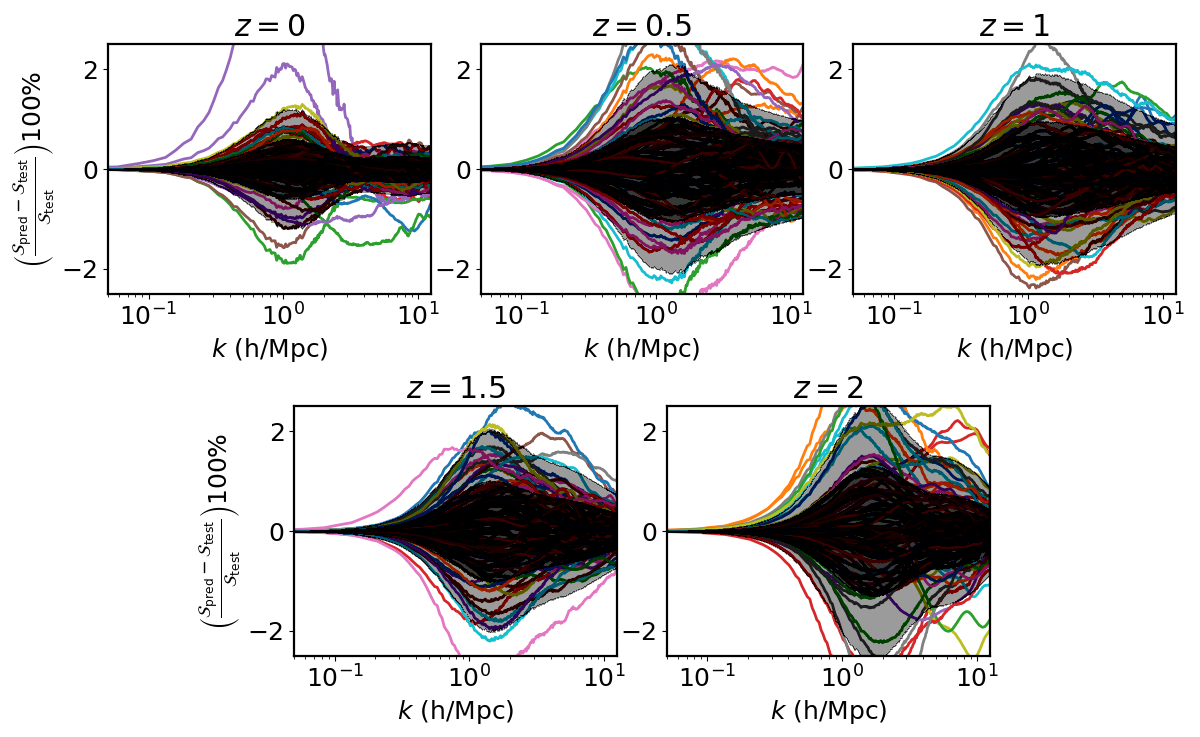
\includegraphics[width=0.85\textwidth,height=0.6\textheight,keepaspectratio]{fig-1.png}
\caption{Figure 1: The percentage error of predicting the \textbackslash{}mathcal\{S\}(k) in the testing set with our emulators at various redshifts are shown using the coloured lines.. The dark and light shaded regions represent the 1-\textbackslash{}sigma and 2-\textbackslash{}sigma regions respectively. [arXiv:2108.08863] Reproduced from arXiv:2108.08863 (extracted with \texttt{get\_paper\_figures}).}
\label{fig:1}
\end{figure}

\begin{figure}[H]
\centering
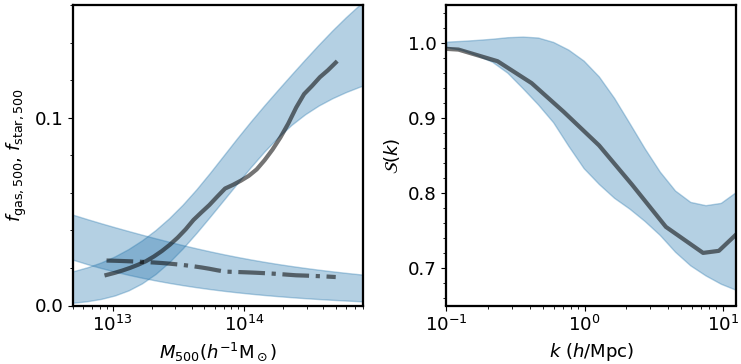
\includegraphics[width=0.85\textwidth,height=0.6\textheight,keepaspectratio]{fig-4.png}
\caption{Figure 3: Comparison between the baryonification model (blue bands) and the hydro-dynamical simulations cosmo-OWLS, BAHAMAS, OWLS, Illustris-TNG, and Horizon-AGN (black lines). For each sub-figure, we show both the gas (f\_\{\textbackslash{}rm gas,500\}; solid line) and stellar (f\_\{\textbackslash{}rm star,500\}; dash-dotted line) fractions as a function of M\_\{500\} (left-hand panel) as well as the baryonic power suppression (\textbackslash{}mathcal\{S\}) as a function of k (right-hand panel). Here the baryonification model is only fitted to the gas and stellar fractions from simulations. The power suppression is then predicted by the baryonific [arXiv:2108.08863] Reproduced from arXiv:2108.08863 (extracted with \texttt{get\_paper\_figures}).}
\label{fig:4}
\end{figure}

\begin{figure}[H]
\centering
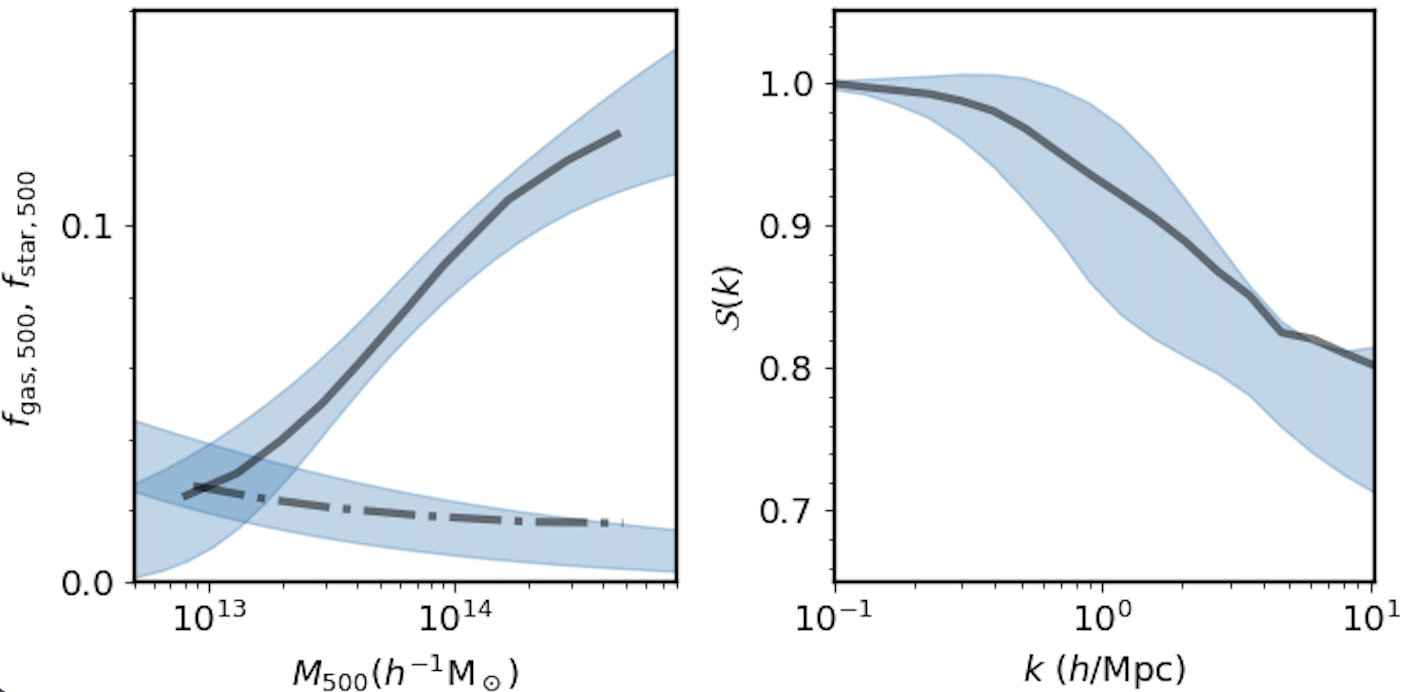
\includegraphics[width=0.85\textwidth,height=0.6\textheight,keepaspectratio]{fig-5.png}
\caption{Figure 3: Comparison between the baryonification model (blue bands) and the hydro-dynamical simulations cosmo-OWLS, BAHAMAS, OWLS, Illustris-TNG, and Horizon-AGN (black lines). For each sub-figure, we show both the gas (f\_\{\textbackslash{}rm gas,500\}; solid line) and stellar (f\_\{\textbackslash{}rm star,500\}; dash-dotted line) fractions as a function of M\_\{500\} (left-hand panel) as well as the baryonic power suppression (\textbackslash{}mathcal\{S\}) as a function of k (right-hand panel). Here the baryonification model is only fitted to the gas and stellar fractions from simulations. The power suppression is then predicted by the baryonific [arXiv:2108.08863] Reproduced from arXiv:2108.08863 (extracted with \texttt{get\_paper\_figures}).}
\label{fig:5}
\end{figure}

\begin{figure}[H]
\centering
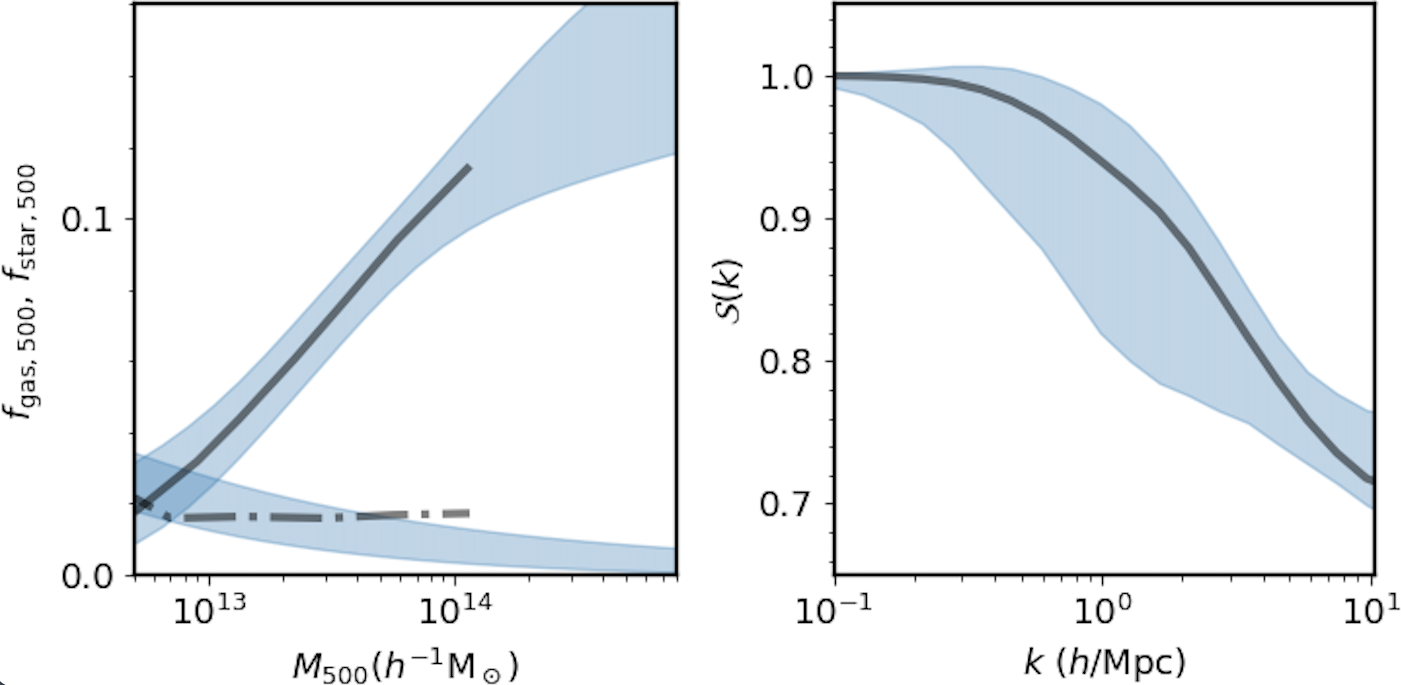
\includegraphics[width=0.85\textwidth,height=0.6\textheight,keepaspectratio]{fig-6.png}
\caption{Figure 3: Comparison between the baryonification model (blue bands) and the hydro-dynamical simulations cosmo-OWLS, BAHAMAS, OWLS, Illustris-TNG, and Horizon-AGN (black lines). For each sub-figure, we show both the gas (f\_\{\textbackslash{}rm gas,500\}; solid line) and stellar (f\_\{\textbackslash{}rm star,500\}; dash-dotted line) fractions as a function of M\_\{500\} (left-hand panel) as well as the baryonic power suppression (\textbackslash{}mathcal\{S\}) as a function of k (right-hand panel). Here the baryonification model is only fitted to the gas and stellar fractions from simulations. The power suppression is then predicted by the baryonific [arXiv:2108.08863] Reproduced from arXiv:2108.08863 (extracted with \texttt{get\_paper\_figures}).}
\label{fig:6}
\end{figure}

\begin{figure}[H]
\centering
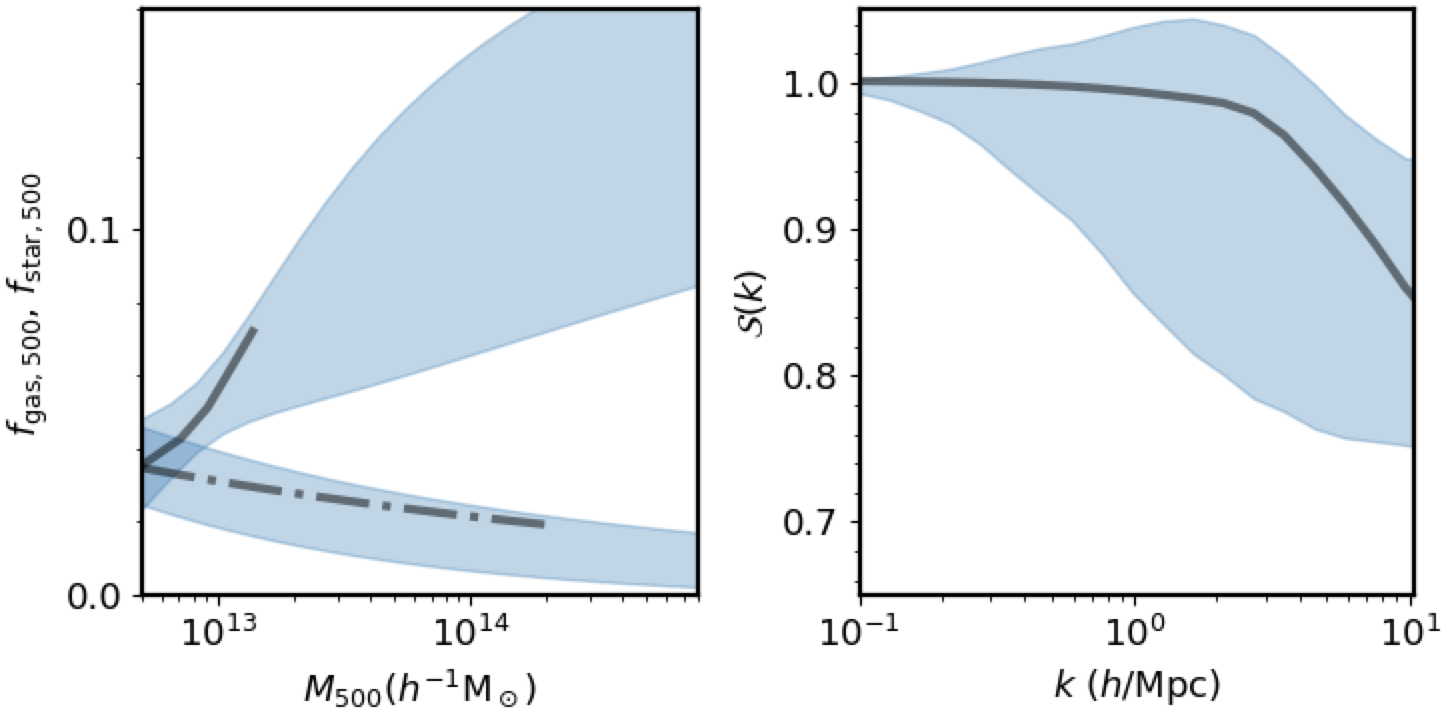
\includegraphics[width=0.85\textwidth,height=0.6\textheight,keepaspectratio]{fig-7.png}
\caption{Figure 3: Comparison between the baryonification model (blue bands) and the hydro-dynamical simulations cosmo-OWLS, BAHAMAS, OWLS, Illustris-TNG, and Horizon-AGN (black lines). For each sub-figure, we show both the gas (f\_\{\textbackslash{}rm gas,500\}; solid line) and stellar (f\_\{\textbackslash{}rm star,500\}; dash-dotted line) fractions as a function of M\_\{500\} (left-hand panel) as well as the baryonic power suppression (\textbackslash{}mathcal\{S\}) as a function of k (right-hand panel). Here the baryonification model is only fitted to the gas and stellar fractions from simulations. The power suppression is then predicted by the baryonific [arXiv:2108.08863] Reproduced from arXiv:2108.08863 (extracted with \texttt{get\_paper\_figures}).}
\label{fig:7}
\end{figure}

\begin{figure}[H]
\centering
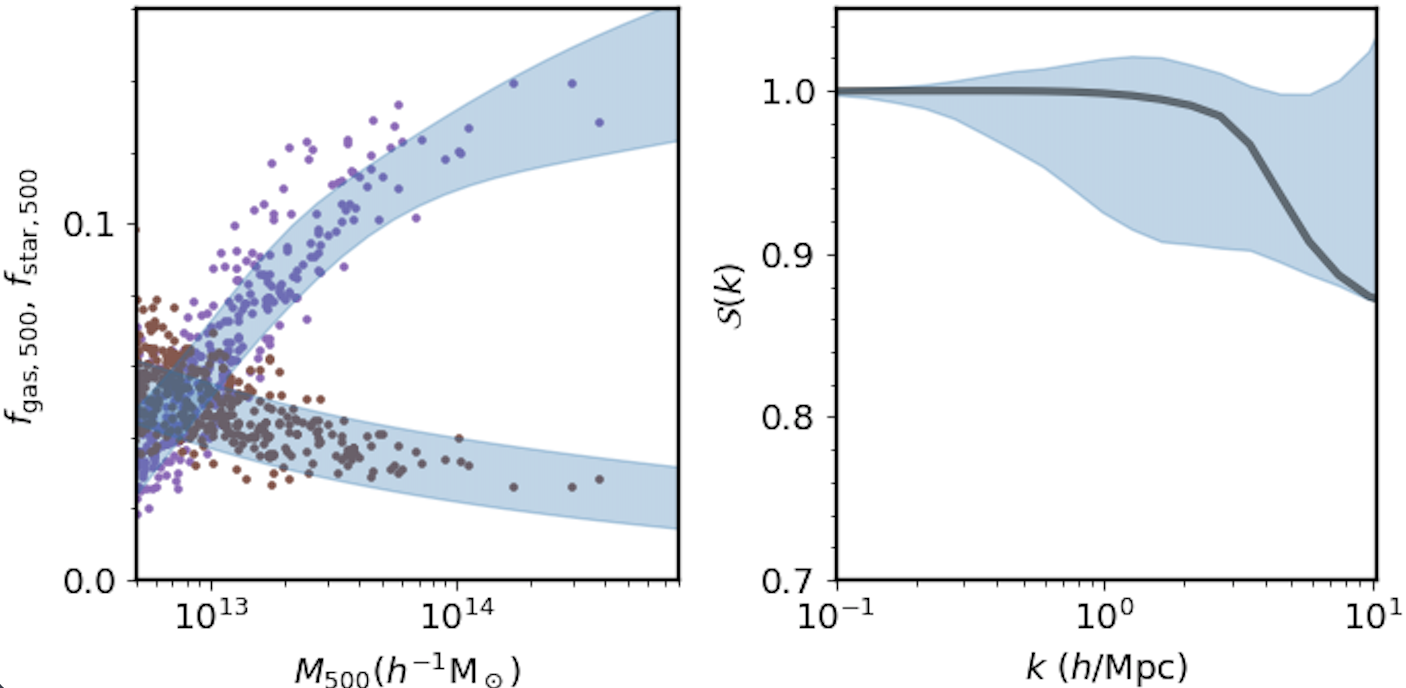
\includegraphics[width=0.85\textwidth,height=0.6\textheight,keepaspectratio]{fig-8.png}
\caption{Figure 3: Comparison between the baryonification model (blue bands) and the hydro-dynamical simulations cosmo-OWLS, BAHAMAS, OWLS, Illustris-TNG, and Horizon-AGN (black lines). For each sub-figure, we show both the gas (f\_\{\textbackslash{}rm gas,500\}; solid line) and stellar (f\_\{\textbackslash{}rm star,500\}; dash-dotted line) fractions as a function of M\_\{500\} (left-hand panel) as well as the baryonic power suppression (\textbackslash{}mathcal\{S\}) as a function of k (right-hand panel). Here the baryonification model is only fitted to the gas and stellar fractions from simulations. The power suppression is then predicted by the baryonific [arXiv:2108.08863] Reproduced from arXiv:2108.08863 (extracted with \texttt{get\_paper\_figures}).}
\label{fig:8}
\end{figure}

\begin{figure}[H]
\centering
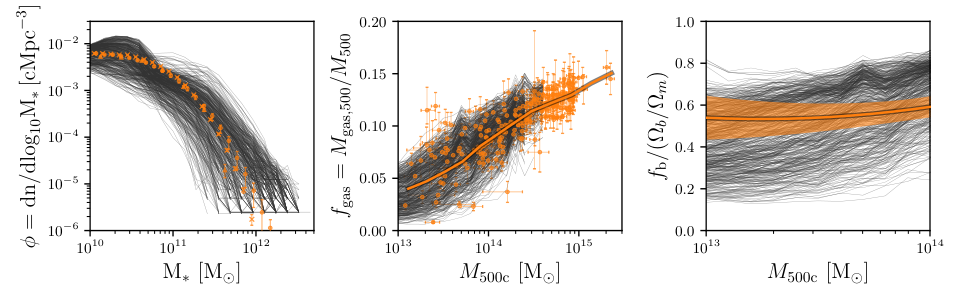
\includegraphics[width=0.85\textwidth,height=0.6\textheight,keepaspectratio]{fig-22.png}
\caption{Figure 1: Galaxy stellar mass function (left), median gas fraction (middle), and median total baryon fraction (right) as a function of halo mass for all 400 simulations at redshift z=0.125. Observational data with their associated uncertainties are shown in orange for the stellar mass function (Baldry et al., 2012; Bernardi et al., 2013; Moustakas et al., 2013; Driver et al., 2022), for the gas fractions of groups and clusters (Vikhlinin et al., 2006; Maughan et al., 2008; Pratt et al., 2009; Rasmussen \& Ponman, 2009; Sun et al., 2009; Lin et al., 2012; Gonzalez et al., 2013; Sanderson et al., [arXiv:2305.09710] Reproduced from arXiv:2305.09710 (extracted with \texttt{get\_paper\_figures}).}
\label{fig:22}
\end{figure}

\begin{figure}[H]
\centering
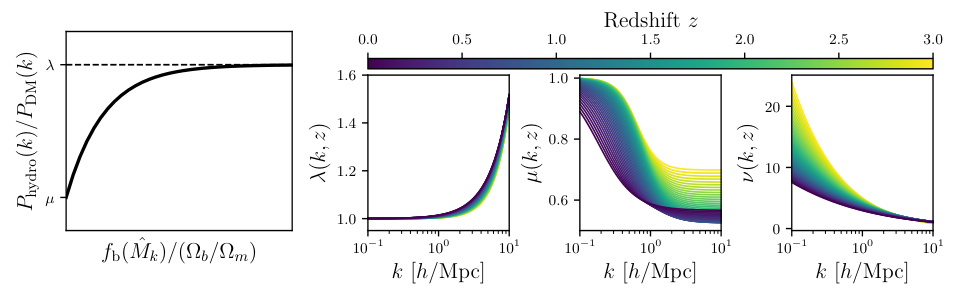
\includegraphics[width=0.85\textwidth,height=0.6\textheight,keepaspectratio]{fig-25.png}
\caption{Figure 7: Left: Illustration of the suppression of the total matter power spectrum as a function of \textbackslash{}tilde\{f\}\_\{b\} as parametrised by Eq. 4. Right: Scale and redshift dependence of the best fit parameters in Table 4. \textbackslash{}lambda(k,z) is the asymptote of the function in Eq. 4 for large \textbackslash{}tilde\{f\}\_\{b\} values, modelled using an exponential functional form (Eq. 6), \textbackslash{}mu(k,z) is the suppression for \textbackslash{}tilde\{f\}\_\{b\}=0, modelled using a logistic functional form (Eq. 7), and \textbackslash{}nu(k,z) is the rate of change, modelled with log-normal functional form (Eq. 8). [arXiv:2305.09710] Reproduced from arXiv:2305.09710 (extracted with \texttt{get\_paper\_figures}).}
\label{fig:25}
\end{figure}

\begin{figure}[H]
\centering
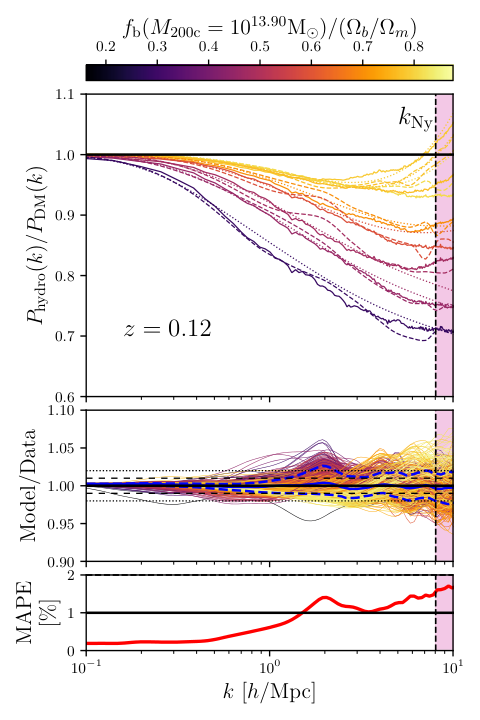
\includegraphics[width=0.85\textwidth,height=0.6\textheight,keepaspectratio]{fig-26.png}
\caption{Figure 8: Top: Fractional impact of baryons on the total matter power spectrum for 8 randomly selected samples from the 400 models. Solid lines use power spectra computed from the simulations. Dashed lines represent the best-fitting model obtained with SP(k) using binned data for the f\_\{b\}-M\_\{\textbackslash{}mathrm\{halo\}\} relation. Dotted lines use a simple power-law fit to the total baryon fraction instead. Colour-coding represents the total baryon fraction of haloes of mass M\_\{200\textbackslash{}mathrm\{c\}\}=10\textasciicircum{}\{13.90\}\textbackslash{}mathrm\{M\}\_\{\textbackslash{}odot\}, which corresponds to the optimal mass at k=1.0\textbackslash{},\{h\textbackslash{},\textbackslash{}mathrm\{Mpc\}\textasciicircum{}\{-1\}\}, i.e. \textbackslash{}hat\{M\}\_\{ [arXiv:2305.09710] Reproduced from arXiv:2305.09710 (extracted with \texttt{get\_paper\_figures}).}
\label{fig:26}
\end{figure}

\end{document}
